   
\documentclass[11pt]{article}

    
    \usepackage[breakable]{tcolorbox}
    \tcbset{nobeforeafter} % prevents tcolorboxes being placing in paragraphs
    \usepackage{float}
    \floatplacement{figure}{H} % forces figures to be placed at the correct location
    
    \usepackage[T1]{fontenc}
    % Nicer default font (+ math font) than Computer Modern for most use cases
    \usepackage{mathpazo}

    % Basic figure setup, for now with no caption control since it's done
    % automatically by Pandoc (which extracts ![](path) syntax from Markdown).
    \usepackage{graphicx}
    % We will generate all images so they have a width \maxwidth. This means
    % that they will get their normal width if they fit onto the page, but
    % are scaled down if they would overflow the margins.
    \makeatletter
    \def\maxwidth{\ifdim\Gin@nat@width>\linewidth\linewidth
    \else\Gin@nat@width\fi}
    \makeatother
%    \let\Oldincludegraphics\includegraphics
    % Set max figure width to be 80% of text width, for now hardcoded.
%    \renewcommand{\includegraphics}[1]{\Oldincludegraphics[width=.8\maxwidth]{#1}}
    % Ensure that by default, figures have no caption (until we provide a
    % proper Figure object with a Caption API and a way to capture that
    % in the conversion process - todo).
%    \usepackage{caption}
%    \DeclareCaptionLabelFormat{nolabel}{}
%    \captionsetup{labelformat=nolabel}

    \usepackage{adjustbox} % Used to constrain images to a maximum size 
    \usepackage{xcolor} % Allow colors to be defined
    \usepackage{enumerate} % Needed for markdown enumerations to work
    \usepackage{geometry} % Used to adjust the document margins
    \usepackage{amsmath} % Equations
    \usepackage{amssymb} % Equations
    \usepackage{textcomp} % defines textquotesingle
    % Hack from http://tex.stackexchange.com/a/47451/13684:
    \AtBeginDocument{%
        \def\PYZsq{\textquotesingle}% Upright quotes in Pygmentized code
    }
    \usepackage{upquote} % Upright quotes for verbatim code
    \usepackage{eurosym} % defines \euro
    \usepackage[mathletters]{ucs} % Extended unicode (utf-8) support
    \usepackage[utf8x]{inputenc} % Allow utf-8 characters in the tex document
    \usepackage{fancyvrb} % verbatim replacement that allows latex
    \usepackage{grffile} % extends the file name processing of package graphics 
                         % to support a larger range 
    % The hyperref package gives us a pdf with properly built
    % internal navigation ('pdf bookmarks' for the table of contents,
    % internal cross-reference links, web links for URLs, etc.)
    \usepackage{hyperref}
    \usepackage{longtable} % longtable support required by pandoc >1.10
    \usepackage{booktabs}  % table support for pandoc > 1.12.2
    \usepackage[inline]{enumitem} % IRkernel/repr support (it uses the enumerate* environment)
    \usepackage[normalem]{ulem} % ulem is needed to support strikethroughs (\sout)
                                % normalem makes italics be italics, not underlines
    \usepackage{mathrsfs}
    

    
    % Colors for the hyperref package
    \definecolor{urlcolor}{rgb}{0,.145,.698}
    \definecolor{linkcolor}{rgb}{.71,0.21,0.01}
    \definecolor{citecolor}{rgb}{.12,.54,.11}

    % ANSI colors
    \definecolor{ansi-black}{HTML}{3E424D}
    \definecolor{ansi-black-intense}{HTML}{282C36}
    \definecolor{ansi-red}{HTML}{E75C58}
    \definecolor{ansi-red-intense}{HTML}{B22B31}
    \definecolor{ansi-green}{HTML}{00A250}
    \definecolor{ansi-green-intense}{HTML}{007427}
    \definecolor{ansi-yellow}{HTML}{DDB62B}
    \definecolor{ansi-yellow-intense}{HTML}{B27D12}
    \definecolor{ansi-blue}{HTML}{208FFB}
    \definecolor{ansi-blue-intense}{HTML}{0065CA}
    \definecolor{ansi-magenta}{HTML}{D160C4}
    \definecolor{ansi-magenta-intense}{HTML}{A03196}
    \definecolor{ansi-cyan}{HTML}{60C6C8}
    \definecolor{ansi-cyan-intense}{HTML}{258F8F}
    \definecolor{ansi-white}{HTML}{C5C1B4}
    \definecolor{ansi-white-intense}{HTML}{A1A6B2}
    \definecolor{ansi-default-inverse-fg}{HTML}{FFFFFF}
    \definecolor{ansi-default-inverse-bg}{HTML}{000000}

    % commands and environments needed by pandoc snippets
    % extracted from the output of `pandoc -s`
    \providecommand{\tightlist}{%
      \setlength{\itemsep}{0pt}\setlength{\parskip}{0pt}}
    \DefineVerbatimEnvironment{Highlighting}{Verbatim}{commandchars=\\\{\}}
    % Add ',fontsize=\small' for more characters per line
    \newenvironment{Shaded}{}{}
    \newcommand{\KeywordTok}[1]{\textcolor[rgb]{0.00,0.44,0.13}{\textbf{{#1}}}}
    \newcommand{\DataTypeTok}[1]{\textcolor[rgb]{0.56,0.13,0.00}{{#1}}}
    \newcommand{\DecValTok}[1]{\textcolor[rgb]{0.25,0.63,0.44}{{#1}}}
    \newcommand{\BaseNTok}[1]{\textcolor[rgb]{0.25,0.63,0.44}{{#1}}}
    \newcommand{\FloatTok}[1]{\textcolor[rgb]{0.25,0.63,0.44}{{#1}}}
    \newcommand{\CharTok}[1]{\textcolor[rgb]{0.25,0.44,0.63}{{#1}}}
    \newcommand{\StringTok}[1]{\textcolor[rgb]{0.25,0.44,0.63}{{#1}}}
    \newcommand{\CommentTok}[1]{\textcolor[rgb]{0.38,0.63,0.69}{\textit{{#1}}}}
    \newcommand{\OtherTok}[1]{\textcolor[rgb]{0.00,0.44,0.13}{{#1}}}
    \newcommand{\AlertTok}[1]{\textcolor[rgb]{1.00,0.00,0.00}{\textbf{{#1}}}}
    \newcommand{\FunctionTok}[1]{\textcolor[rgb]{0.02,0.16,0.49}{{#1}}}
    \newcommand{\RegionMarkerTok}[1]{{#1}}
    \newcommand{\ErrorTok}[1]{\textcolor[rgb]{1.00,0.00,0.00}{\textbf{{#1}}}}
    \newcommand{\NormalTok}[1]{{#1}}
    
    % Additional commands for more recent versions of Pandoc
    \newcommand{\ConstantTok}[1]{\textcolor[rgb]{0.53,0.00,0.00}{{#1}}}
    \newcommand{\SpecialCharTok}[1]{\textcolor[rgb]{0.25,0.44,0.63}{{#1}}}
    \newcommand{\VerbatimStringTok}[1]{\textcolor[rgb]{0.25,0.44,0.63}{{#1}}}
    \newcommand{\SpecialStringTok}[1]{\textcolor[rgb]{0.73,0.40,0.53}{{#1}}}
    \newcommand{\ImportTok}[1]{{#1}}
    \newcommand{\DocumentationTok}[1]{\textcolor[rgb]{0.73,0.13,0.13}{\textit{{#1}}}}
    \newcommand{\AnnotationTok}[1]{\textcolor[rgb]{0.38,0.63,0.69}{\textbf{\textit{{#1}}}}}
    \newcommand{\CommentVarTok}[1]{\textcolor[rgb]{0.38,0.63,0.69}{\textbf{\textit{{#1}}}}}
    \newcommand{\VariableTok}[1]{\textcolor[rgb]{0.10,0.09,0.49}{{#1}}}
    \newcommand{\ControlFlowTok}[1]{\textcolor[rgb]{0.00,0.44,0.13}{\textbf{{#1}}}}
    \newcommand{\OperatorTok}[1]{\textcolor[rgb]{0.40,0.40,0.40}{{#1}}}
    \newcommand{\BuiltInTok}[1]{{#1}}
    \newcommand{\ExtensionTok}[1]{{#1}}
    \newcommand{\PreprocessorTok}[1]{\textcolor[rgb]{0.74,0.48,0.00}{{#1}}}
    \newcommand{\AttributeTok}[1]{\textcolor[rgb]{0.49,0.56,0.16}{{#1}}}
    \newcommand{\InformationTok}[1]{\textcolor[rgb]{0.38,0.63,0.69}{\textbf{\textit{{#1}}}}}
    \newcommand{\WarningTok}[1]{\textcolor[rgb]{0.38,0.63,0.69}{\textbf{\textit{{#1}}}}}
    
    
    % Define a nice break command that doesn't care if a line doesn't already
    % exist.
    \def\br{\hspace*{\fill} \\* }
    % Math Jax compatibility definitions
    \def\gt{>}
    \def\lt{<}
    \let\Oldtex\TeX
    \let\Oldlatex\LaTeX
    \renewcommand{\TeX}{\textrm{\Oldtex}}
    \renewcommand{\LaTeX}{\textrm{\Oldlatex}}
    % Document parameters
    % Document title
    
    
    
    
    
% Pygments definitions
\makeatletter
\def\PY@reset{\let\PY@it=\relax \let\PY@bf=\relax%
    \let\PY@ul=\relax \let\PY@tc=\relax%
    \let\PY@bc=\relax \let\PY@ff=\relax}
\def\PY@tok#1{\csname PY@tok@#1\endcsname}
\def\PY@toks#1+{\ifx\relax#1\empty\else%
    \PY@tok{#1}\expandafter\PY@toks\fi}
\def\PY@do#1{\PY@bc{\PY@tc{\PY@ul{%
    \PY@it{\PY@bf{\PY@ff{#1}}}}}}}
\def\PY#1#2{\PY@reset\PY@toks#1+\relax+\PY@do{#2}}

\expandafter\def\csname PY@tok@w\endcsname{\def\PY@tc##1{\textcolor[rgb]{0.73,0.73,0.73}{##1}}}
\expandafter\def\csname PY@tok@c\endcsname{\let\PY@it=\textit\def\PY@tc##1{\textcolor[rgb]{0.25,0.50,0.50}{##1}}}
\expandafter\def\csname PY@tok@cp\endcsname{\def\PY@tc##1{\textcolor[rgb]{0.74,0.48,0.00}{##1}}}
\expandafter\def\csname PY@tok@k\endcsname{\let\PY@bf=\textbf\def\PY@tc##1{\textcolor[rgb]{0.00,0.50,0.00}{##1}}}
\expandafter\def\csname PY@tok@kp\endcsname{\def\PY@tc##1{\textcolor[rgb]{0.00,0.50,0.00}{##1}}}
\expandafter\def\csname PY@tok@kt\endcsname{\def\PY@tc##1{\textcolor[rgb]{0.69,0.00,0.25}{##1}}}
\expandafter\def\csname PY@tok@o\endcsname{\def\PY@tc##1{\textcolor[rgb]{0.40,0.40,0.40}{##1}}}
\expandafter\def\csname PY@tok@ow\endcsname{\let\PY@bf=\textbf\def\PY@tc##1{\textcolor[rgb]{0.67,0.13,1.00}{##1}}}
\expandafter\def\csname PY@tok@nb\endcsname{\def\PY@tc##1{\textcolor[rgb]{0.00,0.50,0.00}{##1}}}
\expandafter\def\csname PY@tok@nf\endcsname{\def\PY@tc##1{\textcolor[rgb]{0.00,0.00,1.00}{##1}}}
\expandafter\def\csname PY@tok@nc\endcsname{\let\PY@bf=\textbf\def\PY@tc##1{\textcolor[rgb]{0.00,0.00,1.00}{##1}}}
\expandafter\def\csname PY@tok@nn\endcsname{\let\PY@bf=\textbf\def\PY@tc##1{\textcolor[rgb]{0.00,0.00,1.00}{##1}}}
\expandafter\def\csname PY@tok@ne\endcsname{\let\PY@bf=\textbf\def\PY@tc##1{\textcolor[rgb]{0.82,0.25,0.23}{##1}}}
\expandafter\def\csname PY@tok@nv\endcsname{\def\PY@tc##1{\textcolor[rgb]{0.10,0.09,0.49}{##1}}}
\expandafter\def\csname PY@tok@no\endcsname{\def\PY@tc##1{\textcolor[rgb]{0.53,0.00,0.00}{##1}}}
\expandafter\def\csname PY@tok@nl\endcsname{\def\PY@tc##1{\textcolor[rgb]{0.63,0.63,0.00}{##1}}}
\expandafter\def\csname PY@tok@ni\endcsname{\let\PY@bf=\textbf\def\PY@tc##1{\textcolor[rgb]{0.60,0.60,0.60}{##1}}}
\expandafter\def\csname PY@tok@na\endcsname{\def\PY@tc##1{\textcolor[rgb]{0.49,0.56,0.16}{##1}}}
\expandafter\def\csname PY@tok@nt\endcsname{\let\PY@bf=\textbf\def\PY@tc##1{\textcolor[rgb]{0.00,0.50,0.00}{##1}}}
\expandafter\def\csname PY@tok@nd\endcsname{\def\PY@tc##1{\textcolor[rgb]{0.67,0.13,1.00}{##1}}}
\expandafter\def\csname PY@tok@s\endcsname{\def\PY@tc##1{\textcolor[rgb]{0.73,0.13,0.13}{##1}}}
\expandafter\def\csname PY@tok@sd\endcsname{\let\PY@it=\textit\def\PY@tc##1{\textcolor[rgb]{0.73,0.13,0.13}{##1}}}
\expandafter\def\csname PY@tok@si\endcsname{\let\PY@bf=\textbf\def\PY@tc##1{\textcolor[rgb]{0.73,0.40,0.53}{##1}}}
\expandafter\def\csname PY@tok@se\endcsname{\let\PY@bf=\textbf\def\PY@tc##1{\textcolor[rgb]{0.73,0.40,0.13}{##1}}}
\expandafter\def\csname PY@tok@sr\endcsname{\def\PY@tc##1{\textcolor[rgb]{0.73,0.40,0.53}{##1}}}
\expandafter\def\csname PY@tok@ss\endcsname{\def\PY@tc##1{\textcolor[rgb]{0.10,0.09,0.49}{##1}}}
\expandafter\def\csname PY@tok@sx\endcsname{\def\PY@tc##1{\textcolor[rgb]{0.00,0.50,0.00}{##1}}}
\expandafter\def\csname PY@tok@m\endcsname{\def\PY@tc##1{\textcolor[rgb]{0.40,0.40,0.40}{##1}}}
\expandafter\def\csname PY@tok@gh\endcsname{\let\PY@bf=\textbf\def\PY@tc##1{\textcolor[rgb]{0.00,0.00,0.50}{##1}}}
\expandafter\def\csname PY@tok@gu\endcsname{\let\PY@bf=\textbf\def\PY@tc##1{\textcolor[rgb]{0.50,0.00,0.50}{##1}}}
\expandafter\def\csname PY@tok@gd\endcsname{\def\PY@tc##1{\textcolor[rgb]{0.63,0.00,0.00}{##1}}}
\expandafter\def\csname PY@tok@gi\endcsname{\def\PY@tc##1{\textcolor[rgb]{0.00,0.63,0.00}{##1}}}
\expandafter\def\csname PY@tok@gr\endcsname{\def\PY@tc##1{\textcolor[rgb]{1.00,0.00,0.00}{##1}}}
\expandafter\def\csname PY@tok@ge\endcsname{\let\PY@it=\textit}
\expandafter\def\csname PY@tok@gs\endcsname{\let\PY@bf=\textbf}
\expandafter\def\csname PY@tok@gp\endcsname{\let\PY@bf=\textbf\def\PY@tc##1{\textcolor[rgb]{0.00,0.00,0.50}{##1}}}
\expandafter\def\csname PY@tok@go\endcsname{\def\PY@tc##1{\textcolor[rgb]{0.53,0.53,0.53}{##1}}}
\expandafter\def\csname PY@tok@gt\endcsname{\def\PY@tc##1{\textcolor[rgb]{0.00,0.27,0.87}{##1}}}
\expandafter\def\csname PY@tok@err\endcsname{\def\PY@bc##1{\setlength{\fboxsep}{0pt}\fcolorbox[rgb]{1.00,0.00,0.00}{1,1,1}{\strut ##1}}}
\expandafter\def\csname PY@tok@kc\endcsname{\let\PY@bf=\textbf\def\PY@tc##1{\textcolor[rgb]{0.00,0.50,0.00}{##1}}}
\expandafter\def\csname PY@tok@kd\endcsname{\let\PY@bf=\textbf\def\PY@tc##1{\textcolor[rgb]{0.00,0.50,0.00}{##1}}}
\expandafter\def\csname PY@tok@kn\endcsname{\let\PY@bf=\textbf\def\PY@tc##1{\textcolor[rgb]{0.00,0.50,0.00}{##1}}}
\expandafter\def\csname PY@tok@kr\endcsname{\let\PY@bf=\textbf\def\PY@tc##1{\textcolor[rgb]{0.00,0.50,0.00}{##1}}}
\expandafter\def\csname PY@tok@bp\endcsname{\def\PY@tc##1{\textcolor[rgb]{0.00,0.50,0.00}{##1}}}
\expandafter\def\csname PY@tok@fm\endcsname{\def\PY@tc##1{\textcolor[rgb]{0.00,0.00,1.00}{##1}}}
\expandafter\def\csname PY@tok@vc\endcsname{\def\PY@tc##1{\textcolor[rgb]{0.10,0.09,0.49}{##1}}}
\expandafter\def\csname PY@tok@vg\endcsname{\def\PY@tc##1{\textcolor[rgb]{0.10,0.09,0.49}{##1}}}
\expandafter\def\csname PY@tok@vi\endcsname{\def\PY@tc##1{\textcolor[rgb]{0.10,0.09,0.49}{##1}}}
\expandafter\def\csname PY@tok@vm\endcsname{\def\PY@tc##1{\textcolor[rgb]{0.10,0.09,0.49}{##1}}}
\expandafter\def\csname PY@tok@sa\endcsname{\def\PY@tc##1{\textcolor[rgb]{0.73,0.13,0.13}{##1}}}
\expandafter\def\csname PY@tok@sb\endcsname{\def\PY@tc##1{\textcolor[rgb]{0.73,0.13,0.13}{##1}}}
\expandafter\def\csname PY@tok@sc\endcsname{\def\PY@tc##1{\textcolor[rgb]{0.73,0.13,0.13}{##1}}}
\expandafter\def\csname PY@tok@dl\endcsname{\def\PY@tc##1{\textcolor[rgb]{0.73,0.13,0.13}{##1}}}
\expandafter\def\csname PY@tok@s2\endcsname{\def\PY@tc##1{\textcolor[rgb]{0.73,0.13,0.13}{##1}}}
\expandafter\def\csname PY@tok@sh\endcsname{\def\PY@tc##1{\textcolor[rgb]{0.73,0.13,0.13}{##1}}}
\expandafter\def\csname PY@tok@s1\endcsname{\def\PY@tc##1{\textcolor[rgb]{0.73,0.13,0.13}{##1}}}
\expandafter\def\csname PY@tok@mb\endcsname{\def\PY@tc##1{\textcolor[rgb]{0.40,0.40,0.40}{##1}}}
\expandafter\def\csname PY@tok@mf\endcsname{\def\PY@tc##1{\textcolor[rgb]{0.40,0.40,0.40}{##1}}}
\expandafter\def\csname PY@tok@mh\endcsname{\def\PY@tc##1{\textcolor[rgb]{0.40,0.40,0.40}{##1}}}
\expandafter\def\csname PY@tok@mi\endcsname{\def\PY@tc##1{\textcolor[rgb]{0.40,0.40,0.40}{##1}}}
\expandafter\def\csname PY@tok@il\endcsname{\def\PY@tc##1{\textcolor[rgb]{0.40,0.40,0.40}{##1}}}
\expandafter\def\csname PY@tok@mo\endcsname{\def\PY@tc##1{\textcolor[rgb]{0.40,0.40,0.40}{##1}}}
\expandafter\def\csname PY@tok@ch\endcsname{\let\PY@it=\textit\def\PY@tc##1{\textcolor[rgb]{0.25,0.50,0.50}{##1}}}
\expandafter\def\csname PY@tok@cm\endcsname{\let\PY@it=\textit\def\PY@tc##1{\textcolor[rgb]{0.25,0.50,0.50}{##1}}}
\expandafter\def\csname PY@tok@cpf\endcsname{\let\PY@it=\textit\def\PY@tc##1{\textcolor[rgb]{0.25,0.50,0.50}{##1}}}
\expandafter\def\csname PY@tok@c1\endcsname{\let\PY@it=\textit\def\PY@tc##1{\textcolor[rgb]{0.25,0.50,0.50}{##1}}}
\expandafter\def\csname PY@tok@cs\endcsname{\let\PY@it=\textit\def\PY@tc##1{\textcolor[rgb]{0.25,0.50,0.50}{##1}}}

\def\PYZbs{\char`\\}
\def\PYZus{\char`\_}
\def\PYZob{\char`\{}
\def\PYZcb{\char`\}}
\def\PYZca{\char`\^}
\def\PYZam{\char`\&}
\def\PYZlt{\char`\<}
\def\PYZgt{\char`\>}
\def\PYZsh{\char`\#}
\def\PYZpc{\char`\%}
\def\PYZdl{\char`\$}
\def\PYZhy{\char`\-}
\def\PYZsq{\char`\'}
\def\PYZdq{\char`\"}
\def\PYZti{\char`\~}
% for compatibility with earlier versions
\def\PYZat{@}
\def\PYZlb{[}
\def\PYZrb{]}
\makeatother


    % For linebreaks inside Verbatim environment from package fancyvrb. 
    \makeatletter
        \newbox\Wrappedcontinuationbox 
        \newbox\Wrappedvisiblespacebox 
        \newcommand*\Wrappedvisiblespace {\textcolor{red}{\textvisiblespace}} 
        \newcommand*\Wrappedcontinuationsymbol {\textcolor{red}{\llap{\tiny$\m@th\hookrightarrow$}}} 
        \newcommand*\Wrappedcontinuationindent {3ex } 
        \newcommand*\Wrappedafterbreak {\kern\Wrappedcontinuationindent\copy\Wrappedcontinuationbox} 
        % Take advantage of the already applied Pygments mark-up to insert 
        % potential linebreaks for TeX processing. 
        %        {, <, #, %, $, ' and ": go to next line. 
        %        _, }, ^, &, >, - and ~: stay at end of broken line. 
        % Use of \textquotesingle for straight quote. 
        \newcommand*\Wrappedbreaksatspecials {% 
            \def\PYGZus{\discretionary{\char`\_}{\Wrappedafterbreak}{\char`\_}}% 
            \def\PYGZob{\discretionary{}{\Wrappedafterbreak\char`\{}{\char`\{}}% 
            \def\PYGZcb{\discretionary{\char`\}}{\Wrappedafterbreak}{\char`\}}}% 
            \def\PYGZca{\discretionary{\char`\^}{\Wrappedafterbreak}{\char`\^}}% 
            \def\PYGZam{\discretionary{\char`\&}{\Wrappedafterbreak}{\char`\&}}% 
            \def\PYGZlt{\discretionary{}{\Wrappedafterbreak\char`\<}{\char`\<}}% 
            \def\PYGZgt{\discretionary{\char`\>}{\Wrappedafterbreak}{\char`\>}}% 
            \def\PYGZsh{\discretionary{}{\Wrappedafterbreak\char`\#}{\char`\#}}% 
            \def\PYGZpc{\discretionary{}{\Wrappedafterbreak\char`\%}{\char`\%}}% 
            \def\PYGZdl{\discretionary{}{\Wrappedafterbreak\char`\$}{\char`\$}}% 
            \def\PYGZhy{\discretionary{\char`\-}{\Wrappedafterbreak}{\char`\-}}% 
            \def\PYGZsq{\discretionary{}{\Wrappedafterbreak\textquotesingle}{\textquotesingle}}% 
            \def\PYGZdq{\discretionary{}{\Wrappedafterbreak\char`\"}{\char`\"}}% 
            \def\PYGZti{\discretionary{\char`\~}{\Wrappedafterbreak}{\char`\~}}% 
        } 
        % Some characters . , ; ? ! / are not pygmentized. 
        % This macro makes them "active" and they will insert potential linebreaks 
        \newcommand*\Wrappedbreaksatpunct {% 
            \lccode`\~`\.\lowercase{\def~}{\discretionary{\hbox{\char`\.}}{\Wrappedafterbreak}{\hbox{\char`\.}}}% 
            \lccode`\~`\,\lowercase{\def~}{\discretionary{\hbox{\char`\,}}{\Wrappedafterbreak}{\hbox{\char`\,}}}% 
            \lccode`\~`\;\lowercase{\def~}{\discretionary{\hbox{\char`\;}}{\Wrappedafterbreak}{\hbox{\char`\;}}}% 
            \lccode`\~`\:\lowercase{\def~}{\discretionary{\hbox{\char`\:}}{\Wrappedafterbreak}{\hbox{\char`\:}}}% 
            \lccode`\~`\?\lowercase{\def~}{\discretionary{\hbox{\char`\?}}{\Wrappedafterbreak}{\hbox{\char`\?}}}% 
            \lccode`\~`\!\lowercase{\def~}{\discretionary{\hbox{\char`\!}}{\Wrappedafterbreak}{\hbox{\char`\!}}}% 
            \lccode`\~`\/\lowercase{\def~}{\discretionary{\hbox{\char`\/}}{\Wrappedafterbreak}{\hbox{\char`\/}}}% 
            \catcode`\.\active
            \catcode`\,\active 
            \catcode`\;\active
            \catcode`\:\active
            \catcode`\?\active
            \catcode`\!\active
            \catcode`\/\active 
            \lccode`\~`\~ 	
        }
    \makeatother

    \let\OriginalVerbatim=\Verbatim
    \makeatletter
    \renewcommand{\Verbatim}[1][1]{%
        %\parskip\z@skip
        \sbox\Wrappedcontinuationbox {\Wrappedcontinuationsymbol}%
        \sbox\Wrappedvisiblespacebox {\FV@SetupFont\Wrappedvisiblespace}%
        \def\FancyVerbFormatLine ##1{\hsize\linewidth
            \vtop{\raggedright\hyphenpenalty\z@\exhyphenpenalty\z@
                \doublehyphendemerits\z@\finalhyphendemerits\z@
                \strut ##1\strut}%
        }%
        % If the linebreak is at a space, the latter will be displayed as visible
        % space at end of first line, and a continuation symbol starts next line.
        % Stretch/shrink are however usually zero for typewriter font.
        \def\FV@Space {%
            \nobreak\hskip\z@ plus\fontdimen3\font minus\fontdimen4\font
            \discretionary{\copy\Wrappedvisiblespacebox}{\Wrappedafterbreak}
            {\kern\fontdimen2\font}%
        }%
        
        % Allow breaks at special characters using \PYG... macros.
        \Wrappedbreaksatspecials
        % Breaks at punctuation characters . , ; ? ! and / need catcode=\active 	
        \OriginalVerbatim[#1,codes*=\Wrappedbreaksatpunct]%
    }
    \makeatother

    % Exact colors from NB
    \definecolor{incolor}{HTML}{303F9F}
    \definecolor{outcolor}{HTML}{D84315}
    \definecolor{cellborder}{HTML}{CFCFCF}
    \definecolor{cellbackground}{HTML}{F7F7F7}
    
    % prompt
    \newcommand{\prompt}[4]{
        \llap{{\color{#2}[#3]: #4}}\vspace{-1.25em}
    }
    

    
    % Prevent overflowing lines due to hard-to-break entities
    \sloppy 
    % Setup hyperref package
    \hypersetup{
      breaklinks=true,  % so long urls are correctly broken across lines
      colorlinks=true,
      urlcolor=urlcolor,
      linkcolor=linkcolor,
      citecolor=citecolor,
      }
    % Slightly bigger margins than the latex defaults
    
    \geometry{verbose,tmargin=1in,bmargin=1in,lmargin=1in,rmargin=1in}
    
    
    
    
      \usepackage[square,sort,comma,numbers]{natbib}
    
%	\usepackage[font=small,skip=-40pt]{caption}
	\usepackage[]{caption}
	
	\usepackage{booktabs}
	\usepackage{array}
	
   \usepackage{wrapfig}
   
      \usepackage{float}
   \floatstyle{ruled}
   
   \usepackage{subcaption}
    
        \title{Goodreads Recommendations}
        \author{Eitan Angel}


    \begin{document}
    	
	\newcolumntype{H}{>{\setbox0=\hbox\bgroup}c<{\egroup}@{}}
	\newcolumntype{Z}{>{\setbox0=\hbox\bgroup}c<{\egroup}@{\hspace*{-\tabcolsep}}}
    
    \maketitle
 
\tableofcontents
%\newpage

\listoffigures 

\listoftables
 
 \newpage
 
     \hypertarget{introduction}{%
\section{Introduction}\label{introduction}}

%______________________________________________________________________

    \hypertarget{problem}{%
\subsection{Problem: Make Book Recommendations for Goodreads Users}\label{problem}}

\href{https://www.goodreads.com}{Goodreads} is a social site for readers and for book recommendations. In this project we make recommendations to existing users of books they would most enjoy which they have not yet rated. To do so, we use a collaborative filtering filtering approach and compare the error in our recommendations to the error of some baseline models. Once we have made this model it is not so difficult to provide recommendations to new users who are willing to rate a few books. 

%______________________________________________________________________

    \hypertarget{data}{%
\subsection{Data: \href{https://github.com/zygmuntz/goodbooks-10k}{Goodbooks-10k}}\label{data}}

This is a dataset scraped from Goodreads of the 10,000 most popular books (by number of ratings). It contains book ratings by over 50,000 users, as well as user-created tags, including books tagged ``to-read`` and considerable data on the books themselves in both a \texttt{.csv} file and in an archive of \texttt{.xml} files. The basic model will only consider the explicit book ratings although a next step is to find implicit relationships, say among tags and users or books.
    
%______________________________________________________________________
    
    
    \hypertarget{approach}{%
\subsection{Approach: Collaborative Filtering via Matrix Factorization}}

We will use a \href{https://en.wikipedia.org/wiki/Matrix_factorization_(recommender_systems)#Funk_SVD}{Funk SVD}-like collaborative-filtering approach.
First we create a user-book matrix of ratings $V$ (sparsity $\approx$ 99\%). 
Following that, we can use \href{http://scikit-learn.org/stable/modules/generated/sklearn.decomposition.NMF.html}{Non-negative Matrix Factorization} (NMF) to find matrices $W$ and $H$ which decompose $V$ as $V \approx WH$ by minimizing a root-mean-square error (RMSE) between $V$ and $WH$.

Consider $W$ to be matrix of latent user features and $H$ to be a matrix of latent book features. By matrix completion, we mean to consider the matrix $A = WH$ as ``filling in`` those ratings which are blank in $V$.
To make recommendations for a user, return the top-N values in the row of $A$ corresponding to that user (which they have not already rated). We can compare the RMSE matrix factorization techniques to various simpler baseline models.

While we only consider the explicit information of the matrix of user ratings in our model, there are many clear avenues for improvement. A slightly complex model which takes into account user co-likes and co-dislikes is discussed in \cite{tranRegularizingMatrixFactorization2018}. The general idea of modifying matrix completion algorithms to account for implicit information (e.g. tags) began with \href{https://en.wikipedia.org/wiki/Matrix_factorization_(recommender_systems)#SVD++}{Netflix's SVD++}. Matrix completion techniques are surveyed in \cite{ramlatchanSurveyMatrixCompletion2018}.

%In analogy to ElasticNet, we have two hyperparameters to tune (in addition to deciding on a number of latent features). L2-regularization is useful to control precision. L1-regularization is useful for controlling the sparsity of A; without L1-regularization, A is likely not a sparse matrix. Since A is roughly 50,000 x 10,000, we probably need to control sparsity for resource reasons.
%There are various baseline models to compare the NMF model to using RMSE. There may in addition be a way to attain confidence intervals on RMSE.
%While this is presented as an unsupervised problem, it could be made into a supervised problem by considering a random train/cv/test split of the ratings. Since the purpose is to suggest unseen items, perhaps this supervised phrasing gives an additional check on performance beyond RMSE. On the other hand, I have not seen an approach like this in similar problems.

%______________________________________________________________________
%______________________________________________________________________
%______________________________________________________________________
%______________________________________________________________________
%______________________________________________________________________



    \hypertarget{exploratory-data-analysis}{%
\section{Exploratory Data Analysis}\label{exploratory-data-analysis}}
   
   While the dataset has considerable features and metadata on books and tags, we will focus on ratings. The three relevant files are \texttt{books.csv}, \texttt{ratings.csv}, and \texttt{to\_read.csv}.
   
   
   %______________________________________________________________________
   
   
    \hypertarget{books}{%
\subsection{Books}\label{books}}



The file \texttt{books.csv} has a row for each of the 10,000 most rated books on Goodreads and the following 23 columns:
\texttt{
book\_id,
goodreads\_book\_id,
best\_book\_id,
work\_id,          
books\_count,  
isbn,                 
isbn13,             
authors,            
original\_publication\_year,
original\_title,               
title,                        
language\_code,    
average\_rating,     
ratings\_count,       
work\_ratings\_count,
work\_text\_reviews\_count,
ratings\_1,
ratings\_2,
ratings\_3,
ratings\_4,
ratings\_5,
image\_url,
small\_image\_url
}.

We will inspect whether \texttt{average\_rating} is influenced by
other \texttt{books.csv} features, as well as some of the top-rated books, oldest books, most- and least-reviewed books
        
    
\begin{figure}
   \begin{center}
    \adjustimage{max size={0.5\linewidth}{0.5\paperheight}}{./exploration_images/output_12_0.png}
    \end{center}
\caption[Average Rating by Ratings Count]{There is some effect of \texttt{ratings\_count} on
\texttt{average\_rating} -- more popular books are better rated.
     \label{fig:average-rating-ratings-count}
}
\end{figure}    
    
    

\begin{figure}
    \begin{center}
    \adjustimage{max size={0.5\linewidth}{0.5\paperheight}}{./exploration_images/output_13_0.png}
    \end{center}
\caption[Average Rating by Reviews Count]{The number of reviews does not have a significant effect on
\texttt{average\_rating}.}
     \label{fig:average-rating-reviews-count}
\end{figure}


\begin{figure}
    \begin{center}
    \adjustimage{max size={0.5\linewidth}{0.5\paperheight}}{./exploration_images/output_15_0.png}
    \end{center}
    \caption[Average Rating by Publication Year]{The effect of \texttt{original\_publication\_year} on
\texttt{average\_rating} is not significant. Negative values are
books published 1 BCE or earlier.}
     \label{fig:average-rating-reviews-count}
\end{figure}
    
%    
%    \hypertarget{top-10s}{%
%\subsubsection{Top 10s}\label{top-10s}}



%    \hypertarget{most-rated-books}{%
%\paragraph{Most Rated Books}\label{most-rated-books}}

%    We'll use \texttt{work\_ratings\_count}, which are ratings for
%\emph{all} editions, while \texttt{ratings\_count} is for the particular
%popular edition.


\begin{table}
\begin{tabular}{lHlHrHrHZ}
\toprule
                     authors &  year &                                              title & language\_code &  avg\_rating &  ratings\_count &  ratings &  work\_text\_reviews\_count &  ratings\_ratio \\
\midrule
             Suzanne Collins &                     2008.0 &            The Hunger Games (The \ldots &           eng &            4.34 &        4780653 &             4942365 &                   155254 &       0.031413 \\
 J.K. Rowling, Mary GrandPr\'e &                     1997.0 &  Harry Potter and the Sorcerer's\ldots &           eng &            4.44 &        4602479 &             4800065 &                    75867 &       0.015805 \\
             Stephenie Meyer &                     2005.0 &                            Twilight (Twilight, \#1) &         en-US &            3.57 &        3866839 &             3916824 &                    95009 &       0.024257 \\
                  Harper Lee &                     1960.0 &                              To Kill a Mockingbird &           eng &            4.25 &        3198671 &             3340896 &                    72586 &       0.021727 \\
         F. Scott Fitzgerald &                     1925.0 &                                   The Great Gatsby &           eng &            3.89 &        2683664 &             2773745 &                    51992 &       0.018744 \\
                  John Green &                     2012.0 &                             The Fault in Our Stars &           eng &            4.26 &        2346404 &             2478609 &                   140739 &       0.056781 \\
               Veronica Roth &                     2011.0 &                          Divergent (Divergent, \#1) &           eng &            4.24 &        1903563 &             2216814 &                   101023 &       0.045571 \\
              J.R.R. Tolkien &                     1937.0 &                                         The Hobbit &         en-US &            4.25 &        2071616 &             2196809 &                    37653 &       0.017140 \\
                 Jane Austen &                     1813.0 &                                Pride and Prejudice &           eng &            4.24 &        2035490 &             2191465 &                    49152 &       0.022429 \\
               J.D. Salinger &                     1951.0 &                             The Catcher in the Rye &           eng &            3.79 &        2044241 &             2120637 &                    44920 &       0.021182 \\
\bottomrule
\end{tabular}
    \caption[Most Rated Books]{The most popular books on Goodreads.}
     \label{tbl:most-rated-books}
\end{table}
        
%    \hypertarget{most-highly-rated-books}{%
%\paragraph{Most Highly-Rated Books}\label{most-highly-rated-books}}
%
%    

\begin{table}
\begin{tabular}{lHlHrHHHZ}
\toprule
                                    authors &  original\_publication\_year &                                              title & language\_code &  average\_rating &  ratings\_count &  work\_ratings\_count &  work\_text\_reviews\_count &  ratings\_ratio \\
\midrule
                             Bill Watterson &                     2005.0 &                     The Complete Calvin and Hobbes &           eng &            4.82 &          28900 &               29968 &                      861 &       0.028731 \\
                J.K. Rowling, Mary GrandPr\'e &                     2003.0 &  Harry Potter Boxed Set, Books 1-5 \ldots. &           eng &            4.77 &          33220 &               33424 &                      156 &       0.004667 \\
                          Brandon Sanderson &                     2014.0 &     Words of Radiance (The Stormlight \ldots &           eng &            4.77 &          73572 &              108176 &                     7261 &       0.067122 \\
                            Francine Rivers &                     1993.0 &                           Mark of the Lion Trilogy &         en-US &            4.76 &           9081 &                9547 &                      731 &       0.076569 \\
 Anonymous \ldots &                     2002.0 &                                    ESV Study Bible &           eng &            4.76 &           8953 &               10784 &                      262 &       0.024295 \\
                             Bill Watterson &                     1996.0 &  It's a Magical World: A Calvin and \ldots &           eng &            4.75 &          22351 &               23429 &                      264 &       0.011268 \\
                             Bill Watterson &                     1996.0 &  There's Treasure Everywhere: A Calvin \ldots &           eng &            4.74 &          16766 &               17285 &                      149 &       0.008620 \\
                               J.K. Rowling &                     1998.0 &           Harry Potter Boxset (Harry Potter, \#1-7) &           eng &            4.74 &         190050 &              204125 &                     6508 &       0.031882 \\
                               J.K. Rowling &                     2005.0 &       Harry Potter Collection (Harry Potter, \#1-6) &           eng &            4.73 &          24618 &               26274 &                      882 &       0.033569 \\
                             Bill Watterson &                     1992.0 &                The Indispensable Calvin and Hobbes &           eng &            4.73 &          14597 &               16911 &                      325 &       0.019218 \\
\bottomrule
\end{tabular}
    \caption[Most Highly-Rated Books]{Calvin \& Hobbes and Harry Potter dominate the average ratings.}
     \label{tbl:most-rated-books}
\end{table}


        
%    \hypertarget{oldest}{%
%\paragraph{Oldest}\label{oldest}}

\begin{table}
\begin{tabular}{lrlHHHHHZ}
\toprule
                                           authors &  year &                                           title & language\_code &  average\_rating &  ratings\_count &  work\_ratings\_count &  work\_text\_reviews\_count &  ratings\_ratio \\
\midrule
                           Anonymous\ldots &                    -1750.0 &                           The Epic of Gilgamesh &           eng &            3.63 &          44345 &               55856 &                     2247 &       0.040228 \\
                Homer, Robert Fagles \ldots &                     -762.0 &                           The Iliad/The Odyssey &           eng &            4.03 &          47825 &               51098 &                      537 &       0.010509 \\
 Homer, Robert Fagles \ldots. &                     -750.0 &                                       The Iliad &           eng &            3.83 &         241088 &              273565 &                     4763 &       0.017411 \\
 Anonymous \ldots &                     -750.0 &                  The I Ching or Book of Changes &           eng &            4.18 &          12781 &               14700 &                      275 &       0.018707 \\
 Homer, Robert Fagles  \ldots &                     -720.0 &                                     The Odyssey &           eng &            3.73 &         670326 &              710757 &                     8101 &       0.011398 \\
                  Aesop, Laura Harris \ldots &                     -560.0 &                                  Aesop's Fables &           eng &            4.05 &          88508 &               98962 &                     1441 &       0.014561 \\
                           Anonymous, Juan Mascar\'o &                     -500.0 &  The Upanishads: Translations from the Sanskrit &           eng &            4.20 &           7365 &                9667 &                      258 &       0.026689 \\
                            Sun Tzu, Thomas Cleary &                     -500.0 &                                  The Art of War &           eng &            3.95 &         167332 &              203948 &                     6335 &       0.031062 \\
 Anonymous \ldots &                     -500.0 &                                  The Dhammapada &           eng &            4.29 &          12639 &               17114 &                      616 &       0.035994 \\
                               Confucius, D.C. Lau &                     -476.0 &                                    The Analects &           eng &            3.82 &           9807 &               13227 &                      468 &       0.035382 \\
\bottomrule
\end{tabular}
    \caption[Oldest Books]{The oldest books in the dataset.}
     \label{tbl:oldest-books}
\end{table}
%        
%    \hypertarget{greatest-and-least-ratings-ratio}{%
%\paragraph{Greatest and Least Ratings
%Ratio}\label{greatest-and-least-ratings-ratio}}



\begin{table}
\begin{tabular}{lHlHrrHHr}
\toprule
                                  authors &  original\_publication\_year &                                      title & language\_code &  avg &  count &  work\_ratings\_count &  work\_text\_reviews\_count &  ratio \\
\midrule
 Cynthia Hand, Brodi Ashton, \ldots &                     2016.0 &         My Lady Jane (The Lady \ldots &           eng &            4.12 &          12794 &               15433 &                     4228 &       0.274 \\
     Amie Kaufman, Jay Kristoff, \ldots&                     2016.0 &           Gemina (The Illuminae \ldots &           eng &            4.56 &          10960 &               17426 &                     4612 &       0.265 \\
               Amie Kaufman, Jay Kristoff &                     2015.0 &        Illuminae (The Illuminae \ldots &           eng &            4.32 &          44500 &               49187 &                    13008 &       0.264 \\
                             Angie Thomas &                     2017.0 &                            The Hate U Give &           eng &            4.62 &          32610 &               38333 &                     9038 &       0.236 \\
                         Stephanie Garber &                     2017.0 &                                    Caraval &           eng &            3.97 &          30975 &               35821 &                     8360 &       0.233 \\
                            Marissa Meyer &                     2016.0 &                                  Heartless &           eng &            4.06 &          33348 &               37000 &                     8605 &       0.233 \\
                         Sarah Pinborough &                     2017.0 &                            Behind Her Eyes &           eng &            3.77 &          17944 &               21613 &                     5003 &       0.231 \\
                       Julianne Donaldson &                     2012.0 &                Edenbrooke (Edenbrooke \ldots &           eng &            4.34 &          28536 &               30220 &                     6929 &       0.229 \\
                           Pam Mu\~noz Ryan &                     2015.0 &                                       Echo &           eng &            4.36 &          14864 &               15642 &                     3526 &       0.225 \\
                          Victoria Schwab &                     2016.0 &  This Savage Song (Monsters \ldots &           eng &            4.14 &          17210 &               22459 &                     5057 &       0.225 \\
\bottomrule
\end{tabular}
    \caption[Greatest Ratings Ratio]{The ratings ratio is \texttt{work\_text\_reviews\_count} divided by
\texttt{work\_ratings\_count}. The majority of the greatest ratings ratio 
books are romance novels.}
     \label{tbl:greatest-ratings-ratio}
\end{table}


\begin{table}
\begin{tabular}{lHlHrrHHr}
\toprule
                                  authors &  original\_publication\_year &                                      title & language\_code &  avg &  count &  work\_ratings\_count &  work\_text\_reviews\_count &  ratio \\
\midrule
                                 Cynthia J. McGean &                     1997.0 &                                     Henry \& Ramona &           NaN &            4.14 &          11106 &               11106 &                        3 &       0.000270 \\
                  John D. Rateliff, J.R.R. Tolkien &                     2007.0 &   The History of the Hobbit, Part One\ldots &           eng &            3.81 &         108399 &              108445 &                       46 &       0.000424 \\
                                      Frank Miller &                     1991.0 &              Sin City: Una Dura Despedida \ldots &           NaN &            4.21 &           9115 &                9116 &                        4 &       0.000439 \\
                                   Janet Evanovich &                     2002.0 &  Janet Evanovich Three and Four \ldots. &           NaN &            4.34 &          63691 &               63694 &                       39 &       0.000612 \\
                        Dean Koontz, Leigh Nichols &                     2000.0 &         Cold Fire / Hideaway / The Key to \ldots &           eng &            4.16 &          17581 &               17581 &                       11 &       0.000626 \\
                                    Mark Cotta Vaz &                     2011.0 &  The Twilight Saga Breaking Dawn \ldots &           eng &            4.30 &         188136 &              188274 &                      134 &       0.000712 \\
 Richard Lancelyn Green, \ldots &                     1985.0 &  The Further Adventures of Sherlock \ldots &           NaN &            4.40 &          36863 &               36872 &                       36 &       0.000976 \\
                                            Amazon &                     2011.0 &                     Kindle Paperwhite User's Guide &           eng &            3.72 &          15002 &               36650 &                       38 &       0.001037 \\
                                   John   Williams &                     2003.0 &  Harry Potter and the Chamber of \ldots &           NaN &            4.61 &          29409 &               29421 &                       31 &       0.001054 \\
                                      Jen\"o Barcsay &                     1953.0 &                             Anatomy for the Artist &           NaN &            3.97 &          21640 &               21688 &                       24 &       0.001107 \\
\bottomrule
\end{tabular}
    \caption[Least Ratings Ratio]{Books with the least ratings ratio.}
     \label{tbl:least-ratings-ratio}
\end{table}

%______________________________________________________________________
        
    \hypertarget{ratings}{%
\subsection{Ratings}\label{ratings}}

\begin{table}[h]
\centering
  \caption{\texttt{ratings.csv} and \texttt{to\_read.csv}}
  \label{tab:pad-dict}
\begin{subtable}[l]{0.42\linewidth}
\centering
\begin{tabular}{rrr}
\toprule
 user\_id &  book\_id &  rating \\
\midrule
       1 &      258 &       5 \\
       2 &     4081 &       4 \\
       2 &      260 &       5 \\
       2 &     9296 &       5 \\
       2 &     2318 &       3 \\
\bottomrule
\end{tabular}
    \caption[\texttt{ratings.csv}]{\texttt{ratings.csv} consists of 5,976,479 entries, 53,424 users, and 10,000 books.}
     \label{tbl:ratings}
\end{subtable}
%
\begin{subtable}[r]{0.42\linewidth}
\centering
\begin{tabular}{rr}
\toprule
 user\_id &  book\_id \\
\midrule
       9 &        8 \\
      15 &      398 \\
      15 &      275 \\
      37 &     7173 \\
      34 &      380 \\
\bottomrule
\end{tabular}
    \caption[\texttt{to\_read.csv}]{\texttt{to\_read.csv} consists of 912,705 entries, 48,871 unique \texttt{user\_id}s, and 9,986 unique \texttt{book\_id}s.}
     \label{tbl:ratings}
\end{subtable}%
        
\end{table}


\begin{figure}
    \begin{center}
    \adjustimage{max size={0.6\linewidth}{0.6\paperheight}}{./exploration_images/output_38_0.png}
    \end{center}
    \caption[Distribution of User Ratings]{Ratings of 4 or 5 are by far most common.}
     \label{fig:average-rating-reviews-count}
\end{figure}


\begin{figure}
    \begin{center}
    \adjustimage{max size={0.6\linewidth}{0.6\paperheight}}{./exploration_images/output_44_0.png}
    \end{center}
    \caption[Distribution of Ratings by Book]{The distribution of ratings by book in \texttt{ratings.csv} is left
skew. The range is 8--22806 though the interquartile range is 155--503. Since the tail is long we plot the distribution for books with fewer
than 1000 ratings.}
     \label{fig:ratings-by-book}
\end{figure}



\begin{figure}
    \begin{center}
    \adjustimage{max size={0.6\linewidth}{0.6\paperheight}}{./exploration_images/output_48_0.png}
    \end{center}
    \caption[Distribution of Ratings by User]{The range of reviews by user is 19--200.}
     \label{fig:ratings-by-user}
\end{figure}

%______________________________________________________________________
    
    \hypertarget{tags}{%
\subsection{Tags}\label{tags}}

We use the user-generated book tags to assist in interpretation of the model. 
\texttt{book\_tags.csv} has the top 100 user-generated tags for each book along with the tag counts by book.
Most users tag at least one book to-read and almost all books are
tagged to-read by some user.
We can optionally let users decide against recommendations of books tagged to-read.


%______________________________________________________________________
%______________________________________________________________________
%______________________________________________________________________
%______________________________________________________________________
%______________________________________________________________________


    \hypertarget{models}{%
\section{Models}\label{models}}
    
    \hypertarget{ratings-matrix}{%
\subsection{Ratings Matrix}\label{ratings-matrix}}


    First collect the user-book ratings into a
matrix \(V\) with rows indexed by the ordered set of users \(U\),
ordered by \texttt{user\_id}, and columns indexed by the ordered set of
books \(B\), ordered by \texttt{book\_id}. As the set of ratings \(R\)
are integers 1 -- 5, we consider no rating to be a 0 in this
representation. Given the matrix \(V\), a baseline model we consider is
the mean book rating, that is, the mean along columns, as a
recommendation value; these recommendations are identical across users.

\begin{figure}
    \centering
    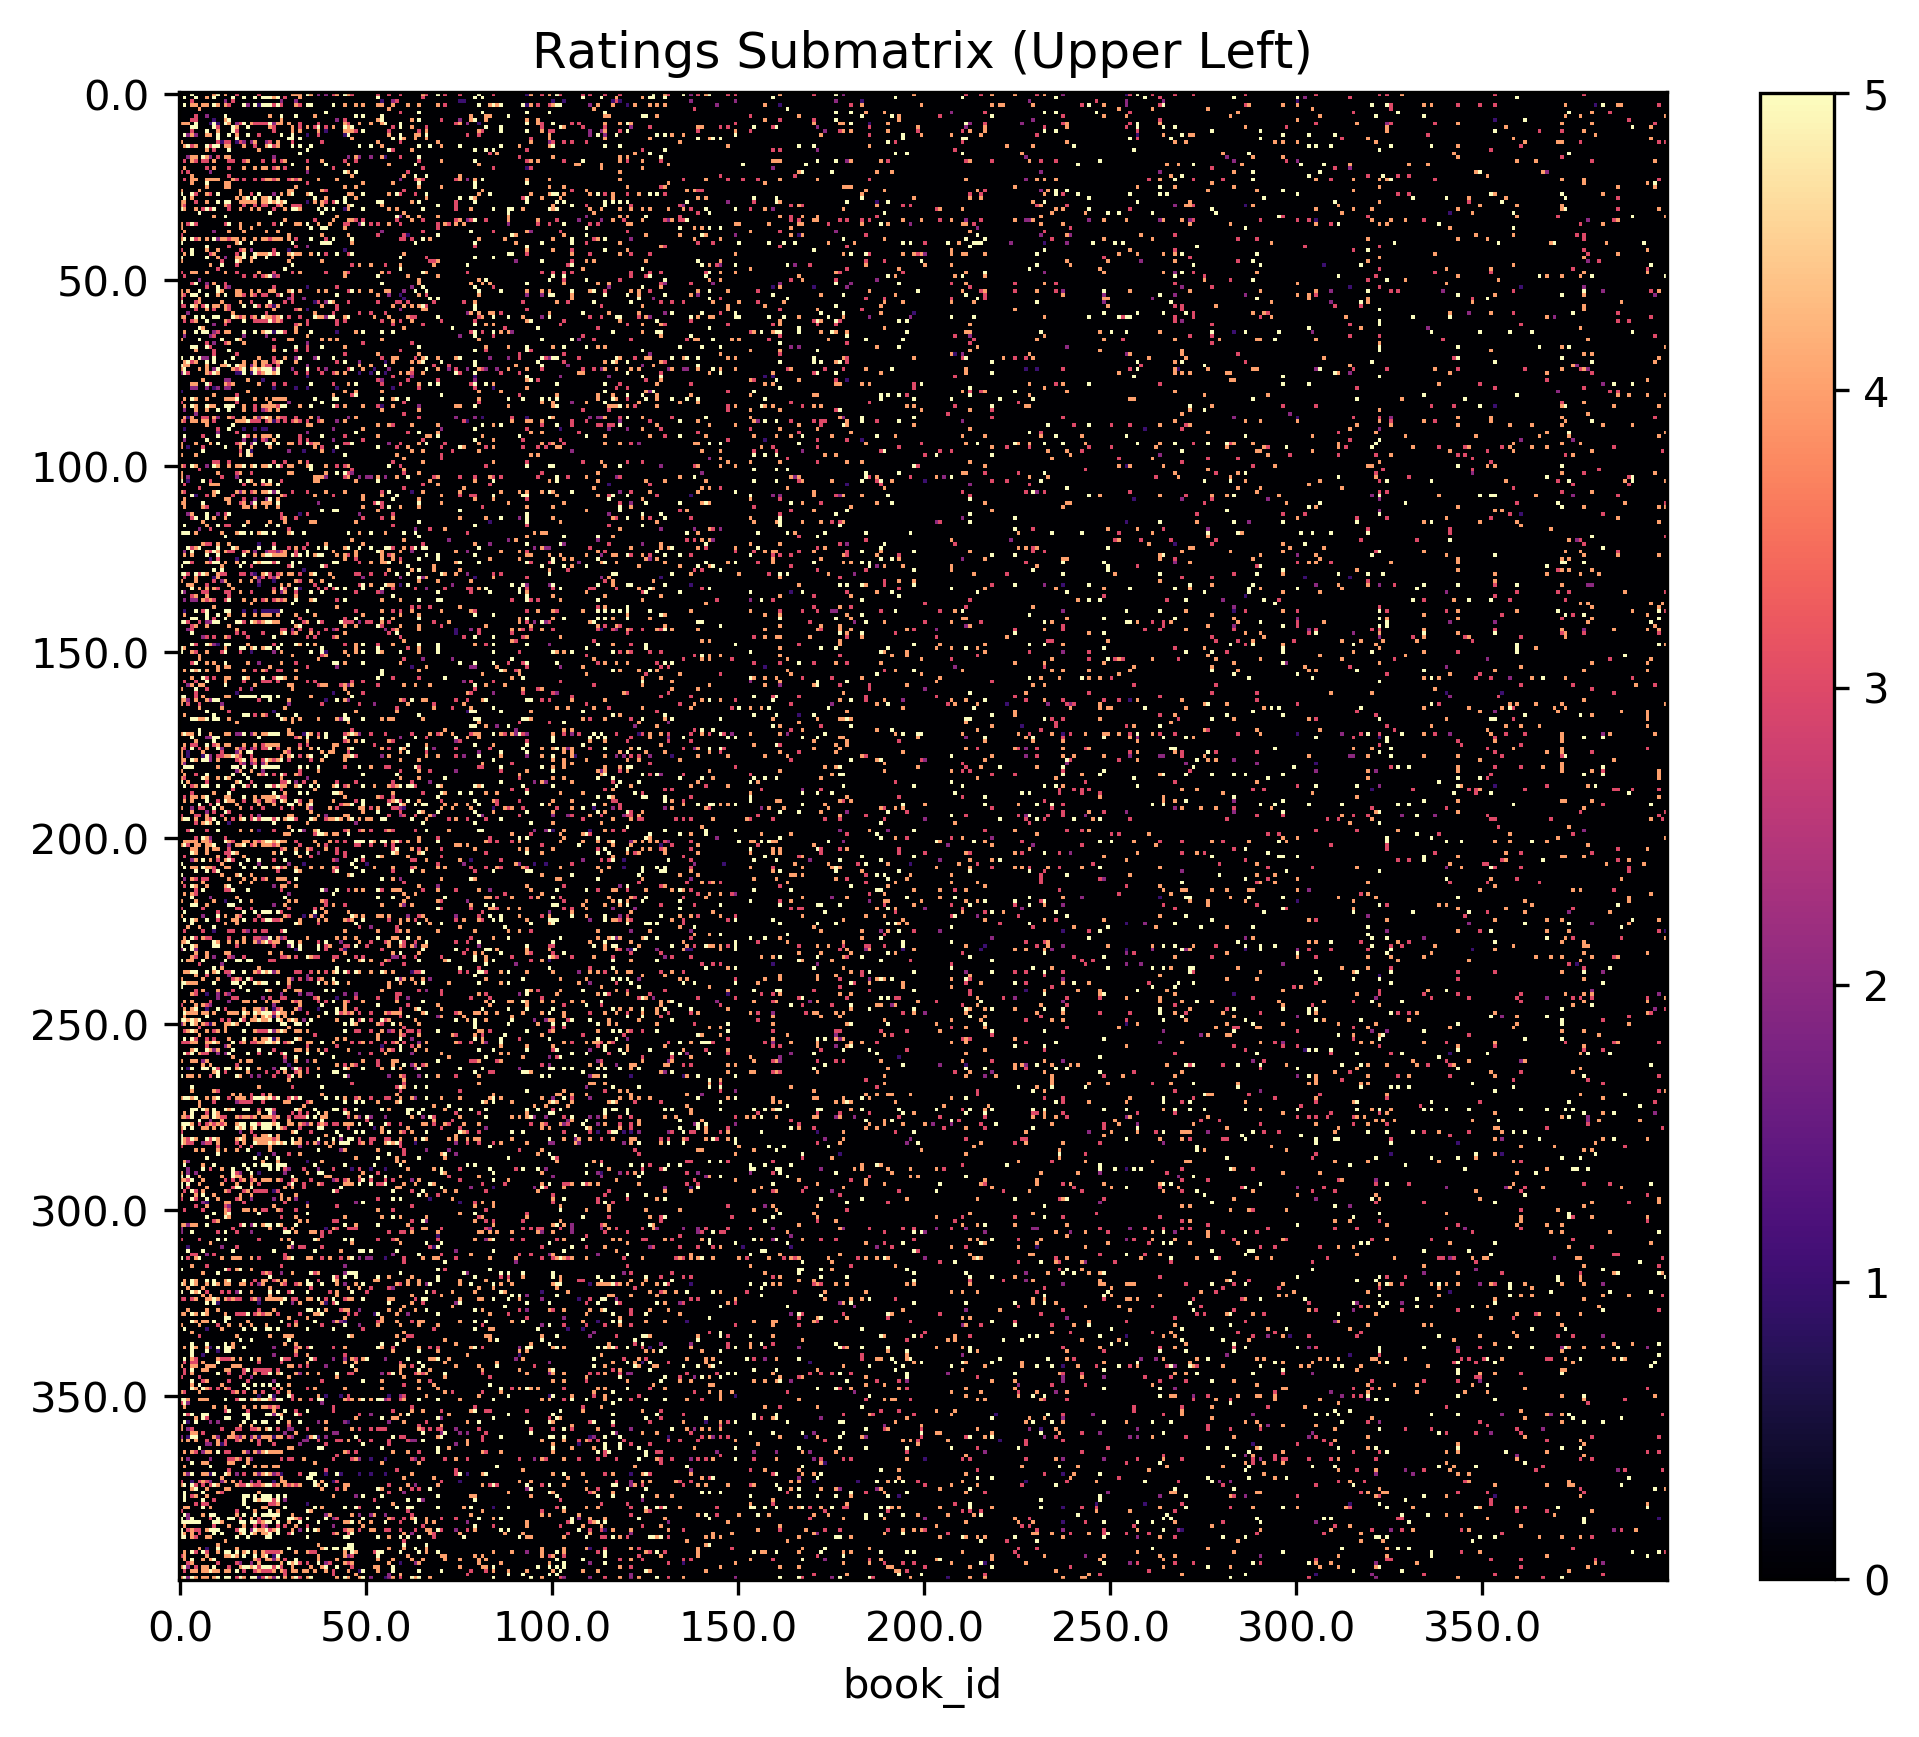
\includegraphics[width=\linewidth]{../image/goodreads-models/ratings-submatrix-upper-left.png}
%    \vspace{-30pt}
    \caption[Ratings Submatrix]{The first 400 rows and columns of the ratings matrix. $\|V\|_F = 9884.39$.}
     \label{fig:ratings-submatrix-upper-left}
\end{figure}


\begin{figure}
    \centering
    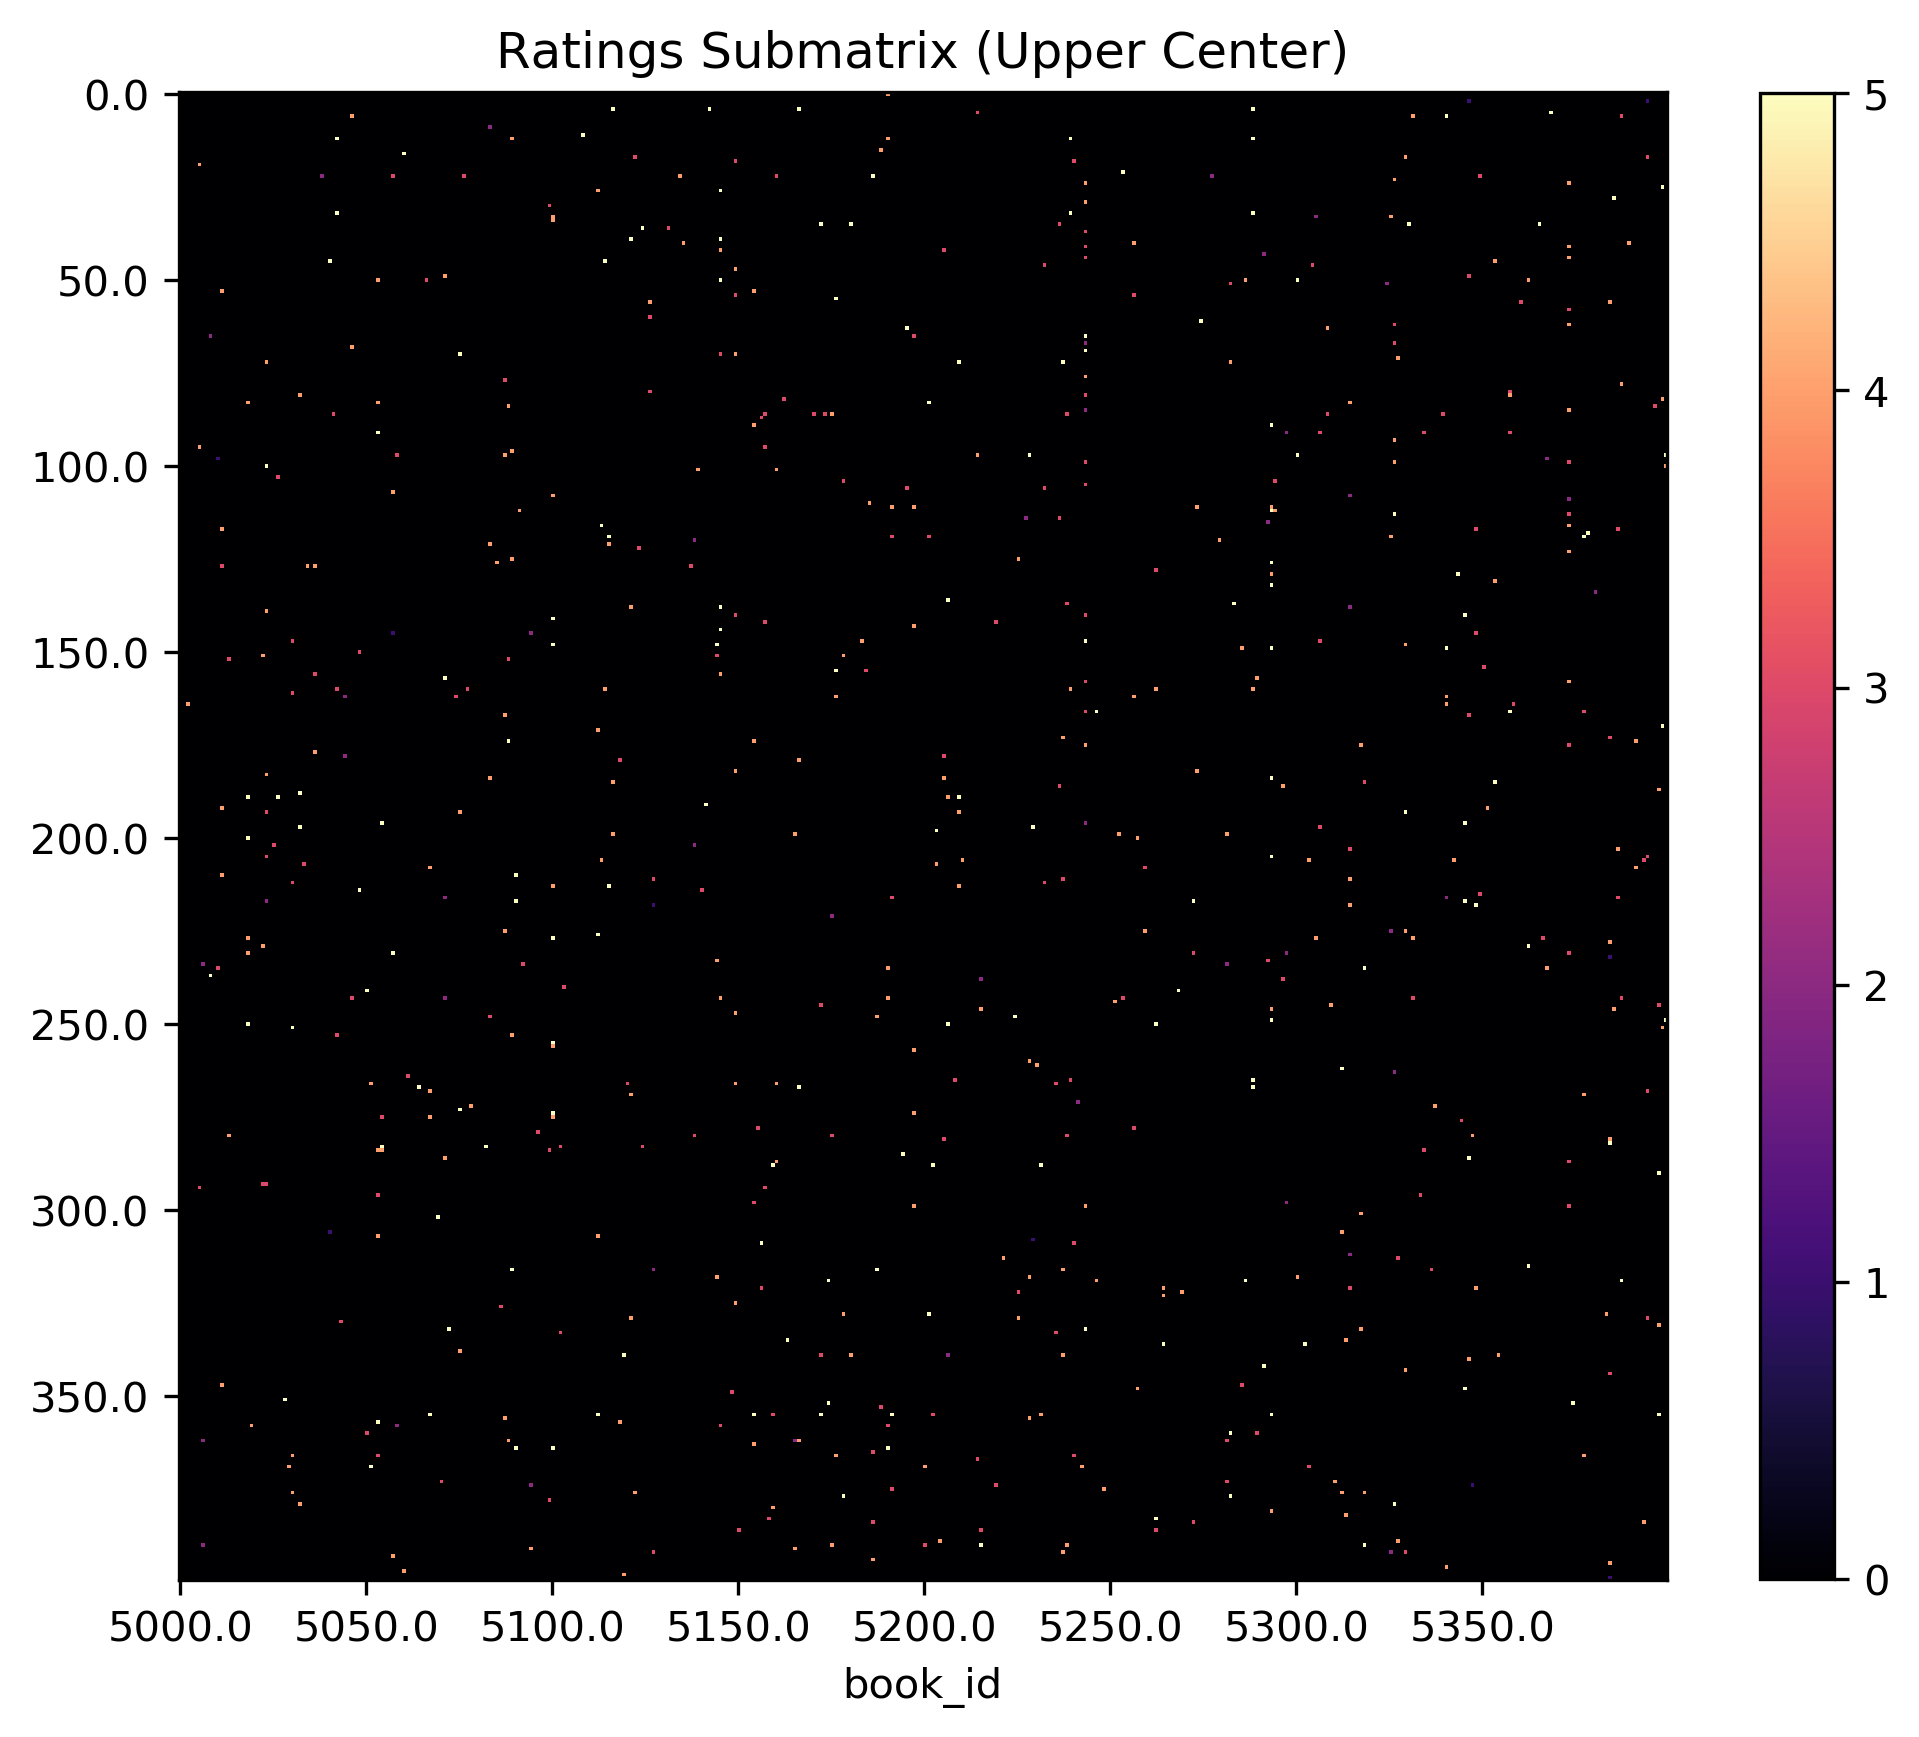
\includegraphics[width=\linewidth]{../image/goodreads-models/ratings-submatrix-upper-center.png}
%    \vspace{-30pt}
    \caption[Ratings Submatrix (Center)]{The upper center of the ratings matrix. \texttt{book\_id} is ordered by overall ratings. The density of the matrix is 1.12\%.}
     \label{fig:ratings-submatrix-upper-left-center}
\end{figure}



    Denote the number of users and books by \(n_u = |U|\) and \(n_b = |B|\)
respectively. The models we construct are matrix factorizations of
\(V \in \mathsf{M}_{n_u \times n_b} (R)\), where \(R\) is the set of
rating values. A choice of the number of latent factors, \(k\), as well
as hyperparameter choices, determine a \emph{matrix factorization
model}, which is a factorization of \(V\) into a matrix
\(W \in \mathsf{M}_{n_u \times k} (\mathbb{R}_{\geq 0})\) and a matrix
\(H \in \mathsf{M}_{k \times n_b} (\mathbb{R}_{\geq 0})\) such that
\(V \approx WH\).

    To be more explicit, we represent
\(V \in \mathsf{M}_{n_u \times n_b} (\mathbb{R}_{\geq 0})\) and use the
\href{https://scikit-learn.org/stable/modules/decomposition.html\#non-negative-matrix-factorization-nmf-or-nnmf}{non-negative
matrix factorization} implementation of scikit-learn,
\href{https://scikit-learn.org/stable/modules/generated/sklearn.decomposition.NMF.html}{sklearn.decomposition.NMF},
to return two matrices \(W\) and \(H\) minimizing the loss function 
\begin{equation} \label{eq:loss-fcn}
\mathcal{L} = \frac{1}{2} \| V - WH \|_F^2,
\end{equation}
where \(\| \bullet \|_F\) is the Frobenius norm \[
\| X \|_F = \sqrt{ \sum_{i, j} X_{ij}^2},
\] that is, the \(L2\)-norm.
\cite{leeAlgorithmsNonnegativeMatrix2001} describes the algorithms used by scikit-learn for matrix
factorization.

In minimizing \(\mathcal{L}\), we are minimizing the root-mean-square
error (RMSE) between \(V\) and \(WH\). In analogy to
\href{https://scikit-learn.org/stable/modules/linear_model.html\#elastic-net}{ElasticNet},
we also explore \(L1\)- and \(L2\)-regularization in
\href{}{hyperparameters}, in which we minimize the loss function 
\begin{equation} \label{eq:reg-loss-fcn}
\mathcal{L}_{\text{reg}} = \frac{1}{2} \| V - WH \|_F^2 + \lambda_1 (\|W\|_1 + \|H\|_1) + \lambda_2 \cdot \frac{1}{2} (\|W\|_F^2 + \|H\|_F^2),
\end{equation} where \(\| \bullet \|_1\) is the \(L1\)-norm \[
\| X \|_1 = \sum_{i, j} |X_{ij}|
\] and \(\lambda_1, \lambda_2 \in \mathbb{R}_{\geq 0}\) are
hyperparameters.

\cite{ramlatchanSurveyMatrixCompletion2018} is a helpful survey of matrix factorization techniques for recommendation which suggests that $L2$-regularization is helpful to prevent overfitting while $L1$-regularization can control density. We examine some effects of regularization in \ref{hyperparameters}.


%______________________________________________________________________
    

    \hypertarget{baseline-model}{%
\subsection{Baseline Model}\label{baseline-model}}

    As a baseline model, take the mean rating for each book as the value along each column of the
ratings matrix $V$. This yields a vector of length $n_b$ which makes uniform predictions across users.
A plot of the baseline model alongside the ratings matrix is in Figure \ref{fig:baseline-matrix}.

The RMSE of the baseline model is $9584.66$, which is a markedly lower score than $\|V\|_F = 9884.39$.
A lower score does mean that the baseline model does in fact approximate $V$.
Scores are lower when we subtract matrices from $V$ which have entries closer to $V$'s entires (in the $L2$ sense).


\begin{figure}[t]
  %  \centering
    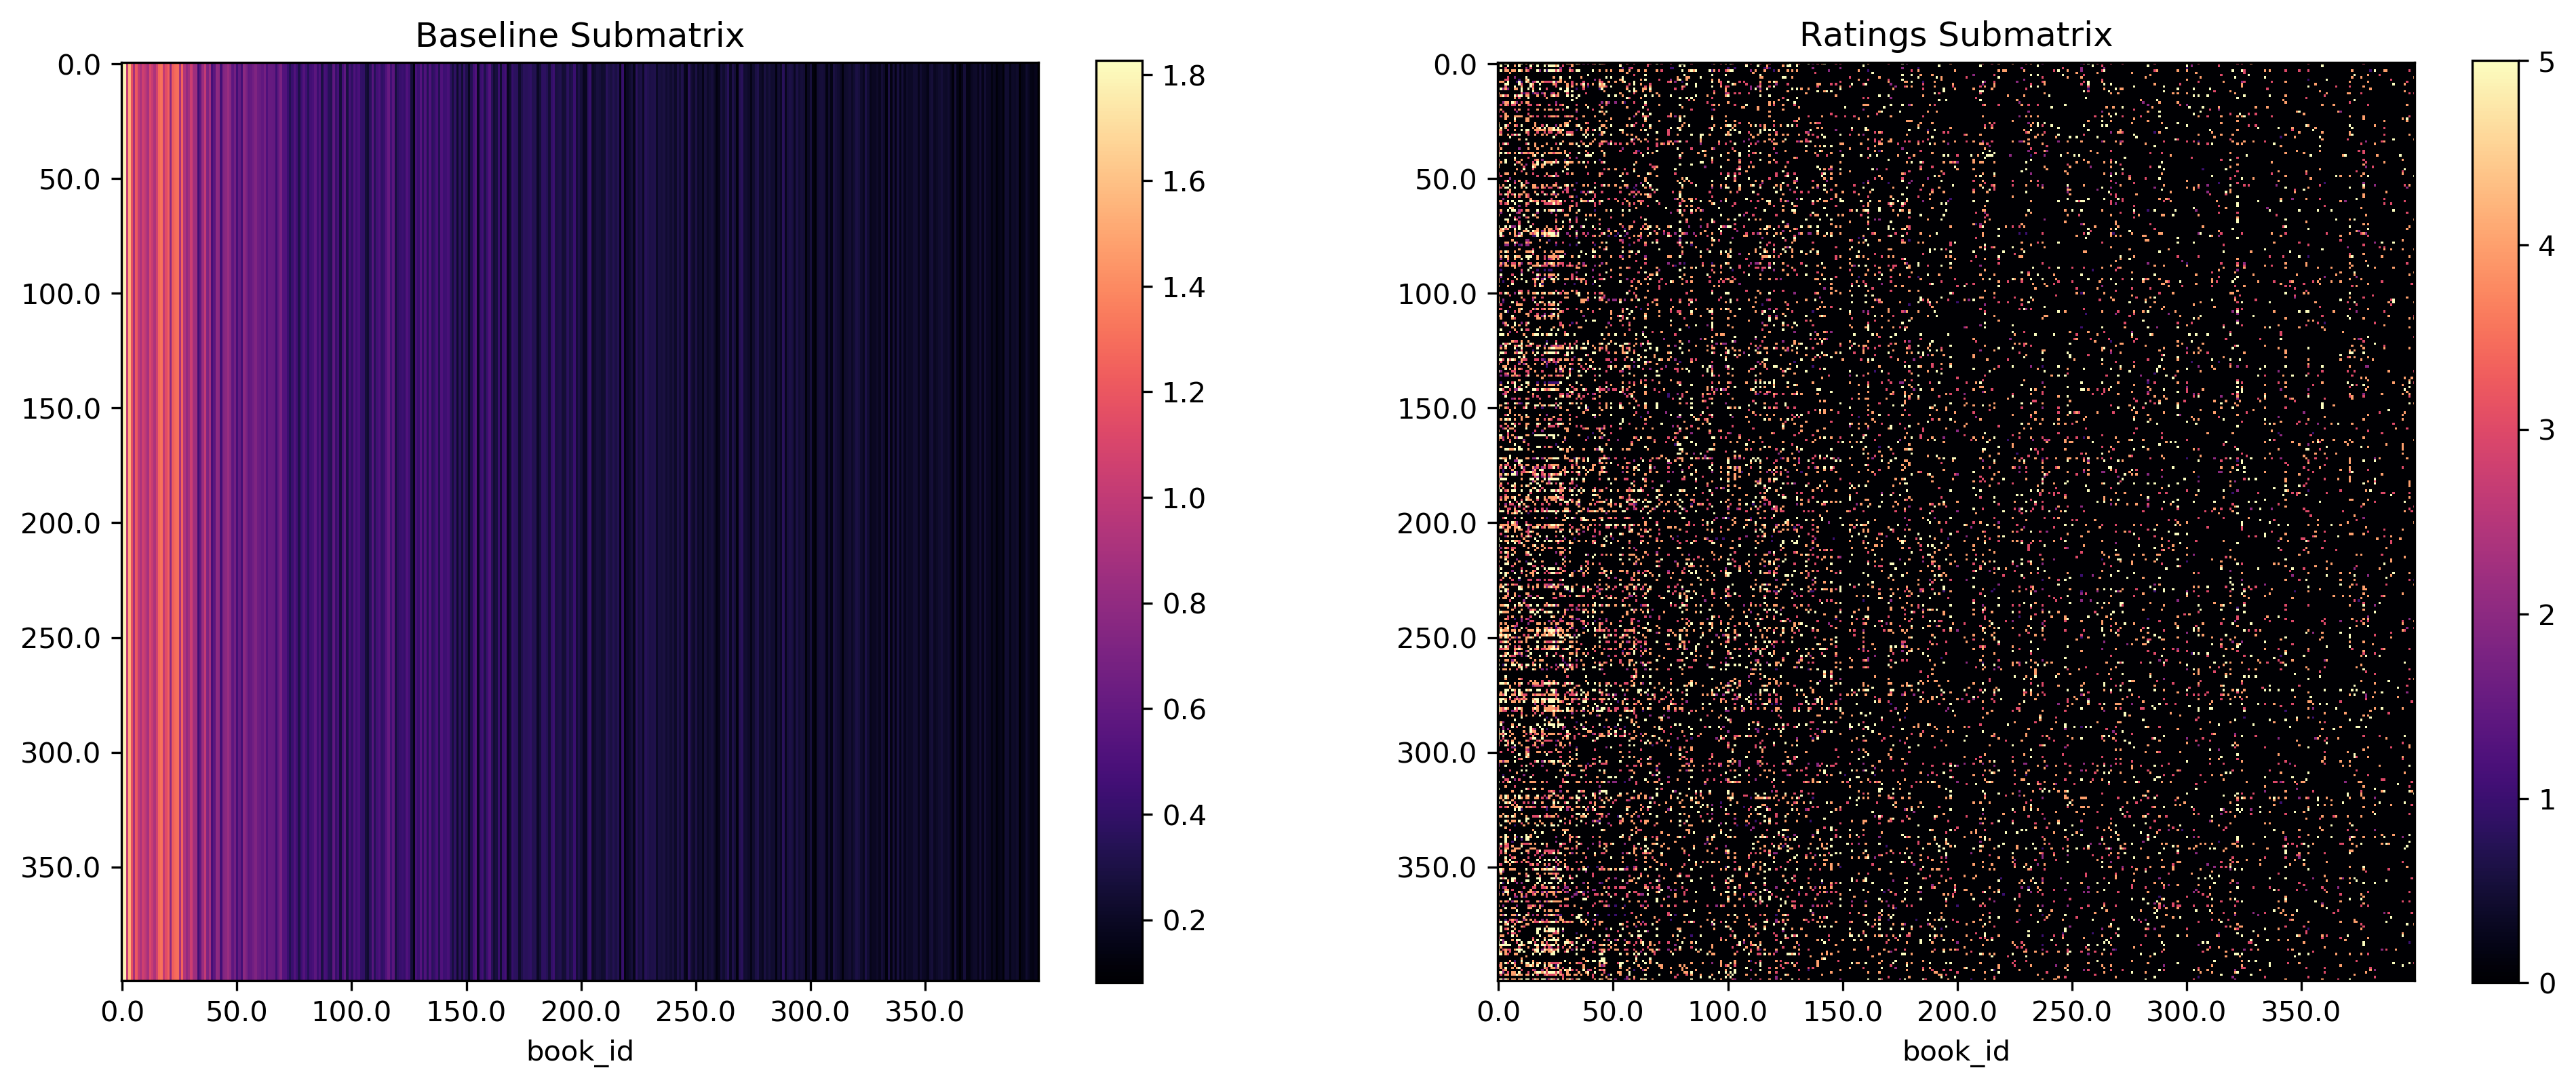
\includegraphics[width=\linewidth]{../image/goodreads-models/baseline-matrix.png}
%    \vspace{-30pt}
    \caption[Baseline matrix]{The mean book rating along each column including no ratings. The RMSE is 9584.66.}
     \label{fig:baseline-matrix}
\end{figure}



%______________________________________________________________________


\newpage

    \hypertarget{factorizations}{%
\subsection{Factorizations}\label{factorizations}}


\begin{wrapfigure}{r}{0.1\textwidth}
    \centering
    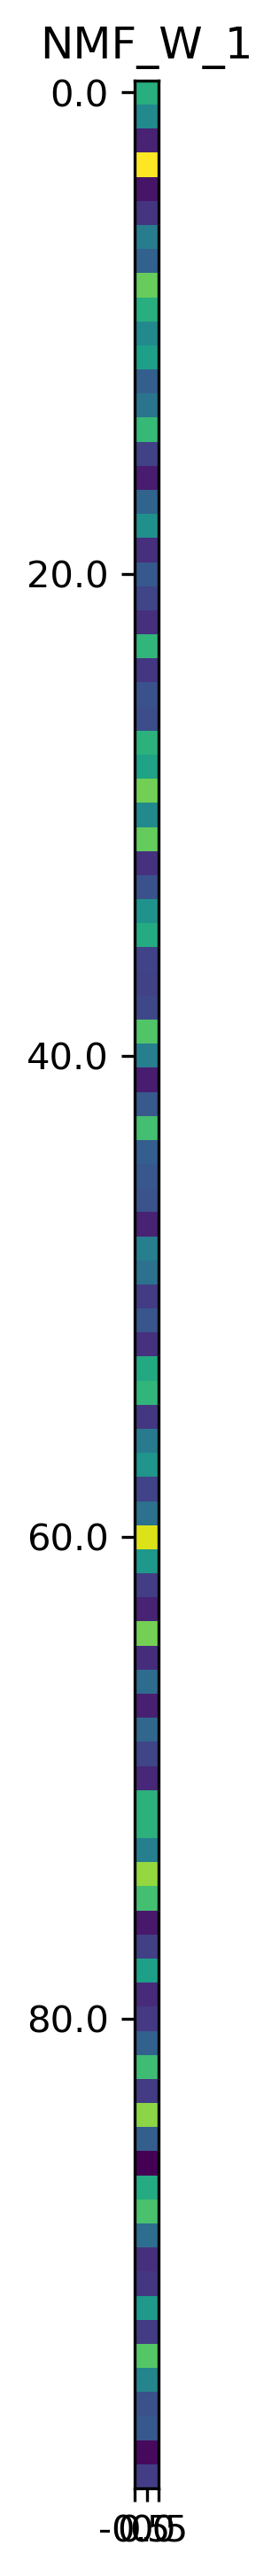
\includegraphics[height=0.9\textwidth, trim=0.2cm 0cm 0.2cm 0cm]{../image/goodreads-models/nmf-W-1.png}
%    \vspace{-30pt}
    \caption[NMF-W-1]{%User preferences ($k=1$)
    }
     \label{fig:nmf-W-1}
\end{wrapfigure}

    We can think of \(W\) as a matrix of \emph{user preferences} for book profiles.
A row \(w_u\) of \(W\) is a vector of length \(k\) which describes the
degree to which each of the \(k\) latent factors influences user
preferences for books. Similarly, we can think of \(H\) as a matrix of \emph{books preferenced} by user profiles;
a column \(h_b\) of \(H\) describes
the degree to which each of the \(k\) latent factors influences that
book's preferences by users.
The dot product \(a_{ub} = w_u h_b^T\) captures the correlation between
user \(u\) and and book \(b\); we consider the matrix \(A = WH\) to be a ``completion'' of \(V\).

There are a few advantages and interpretations of matrix factorization.
\begin{itemize}
\item While a dense matrix of size $n_u \times n_b$ is a few GB, for low $k$, $H$ and $W$ are only a few MB.
\item Since $H$ and $W$ are (for $k < n_u, n_b$) low-rank matrices relative to the size of $V$, matrix factorization
can be considered a dimensionality reduction technique.
\item Matrix factorization has various equivalencies with $K$-means clustering, as described in \cite{dingEquivalenceNonnegativeMatrix2005}.
\item We interpret the latent factors as clusterings, which is the justification for topic modeling in section \ref{topic-extraction}.
\item The latent factors, $H$ and $W$, can be used as training vectors for other models besides matrix completions.
\end{itemize}


%______________________________________________________________________





%______________________________________________________________________

    \hypertarget{k1}{%
\subsubsection{\texorpdfstring{\(k=1\)}{k=1}}\label{k1}}




Choosing a number of latent factors \(k=1\) acts as a sort of baseline
model as well. In this case \(H\) is a vector of book ratings aggregated
by user -- while \(W\) gives the component of each user in the \(H\)
`direction'. In other words, \(W\) describes how `close' each user's
ratings are to the aggregated book ratings. The vector \(H\) is highly
correlated to the column means of the baseline model, so recommendations
from these two models are very similar, but the \(k=1\) model scores
better since it also takes into account how much each user's ratings are
correlated to the aggregated book ratings. We now have not only a row
vector of book rating means but a column vector of user correlations to
the aggregated book ratings.


\begin{figure}[b]
  %  \centering
    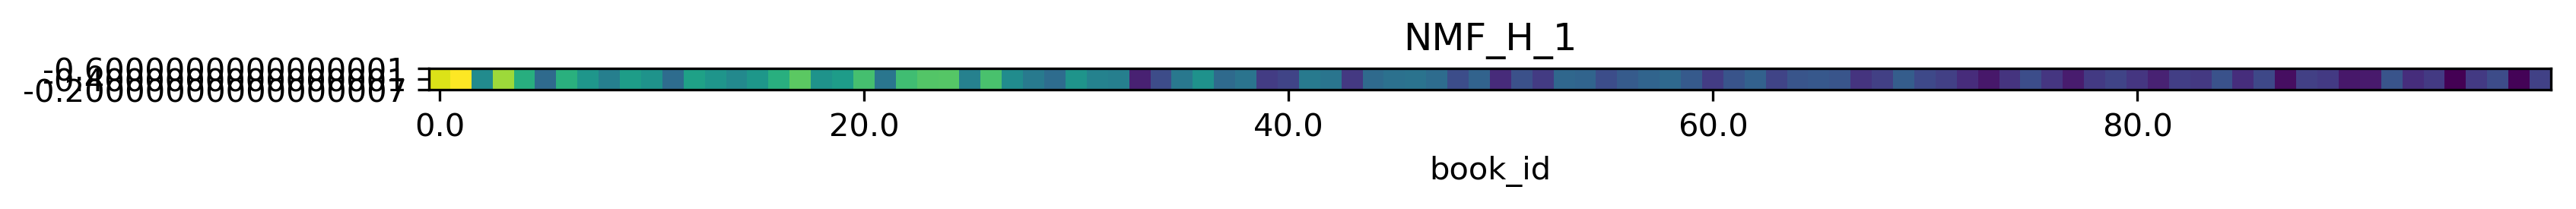
\includegraphics[width=0.9\textwidth, trim=4cm 0cm 0cm 0cm, clip]{../image/goodreads-models/nmf-H-1.png}
%    \vspace{-30pt}
    \caption[NMF-H-1]{A portion of the book preferenced matrix ($k=1$).}
     \label{fig:nmf-H-1}
\end{figure}



\begin{figure}
  %  \centering
    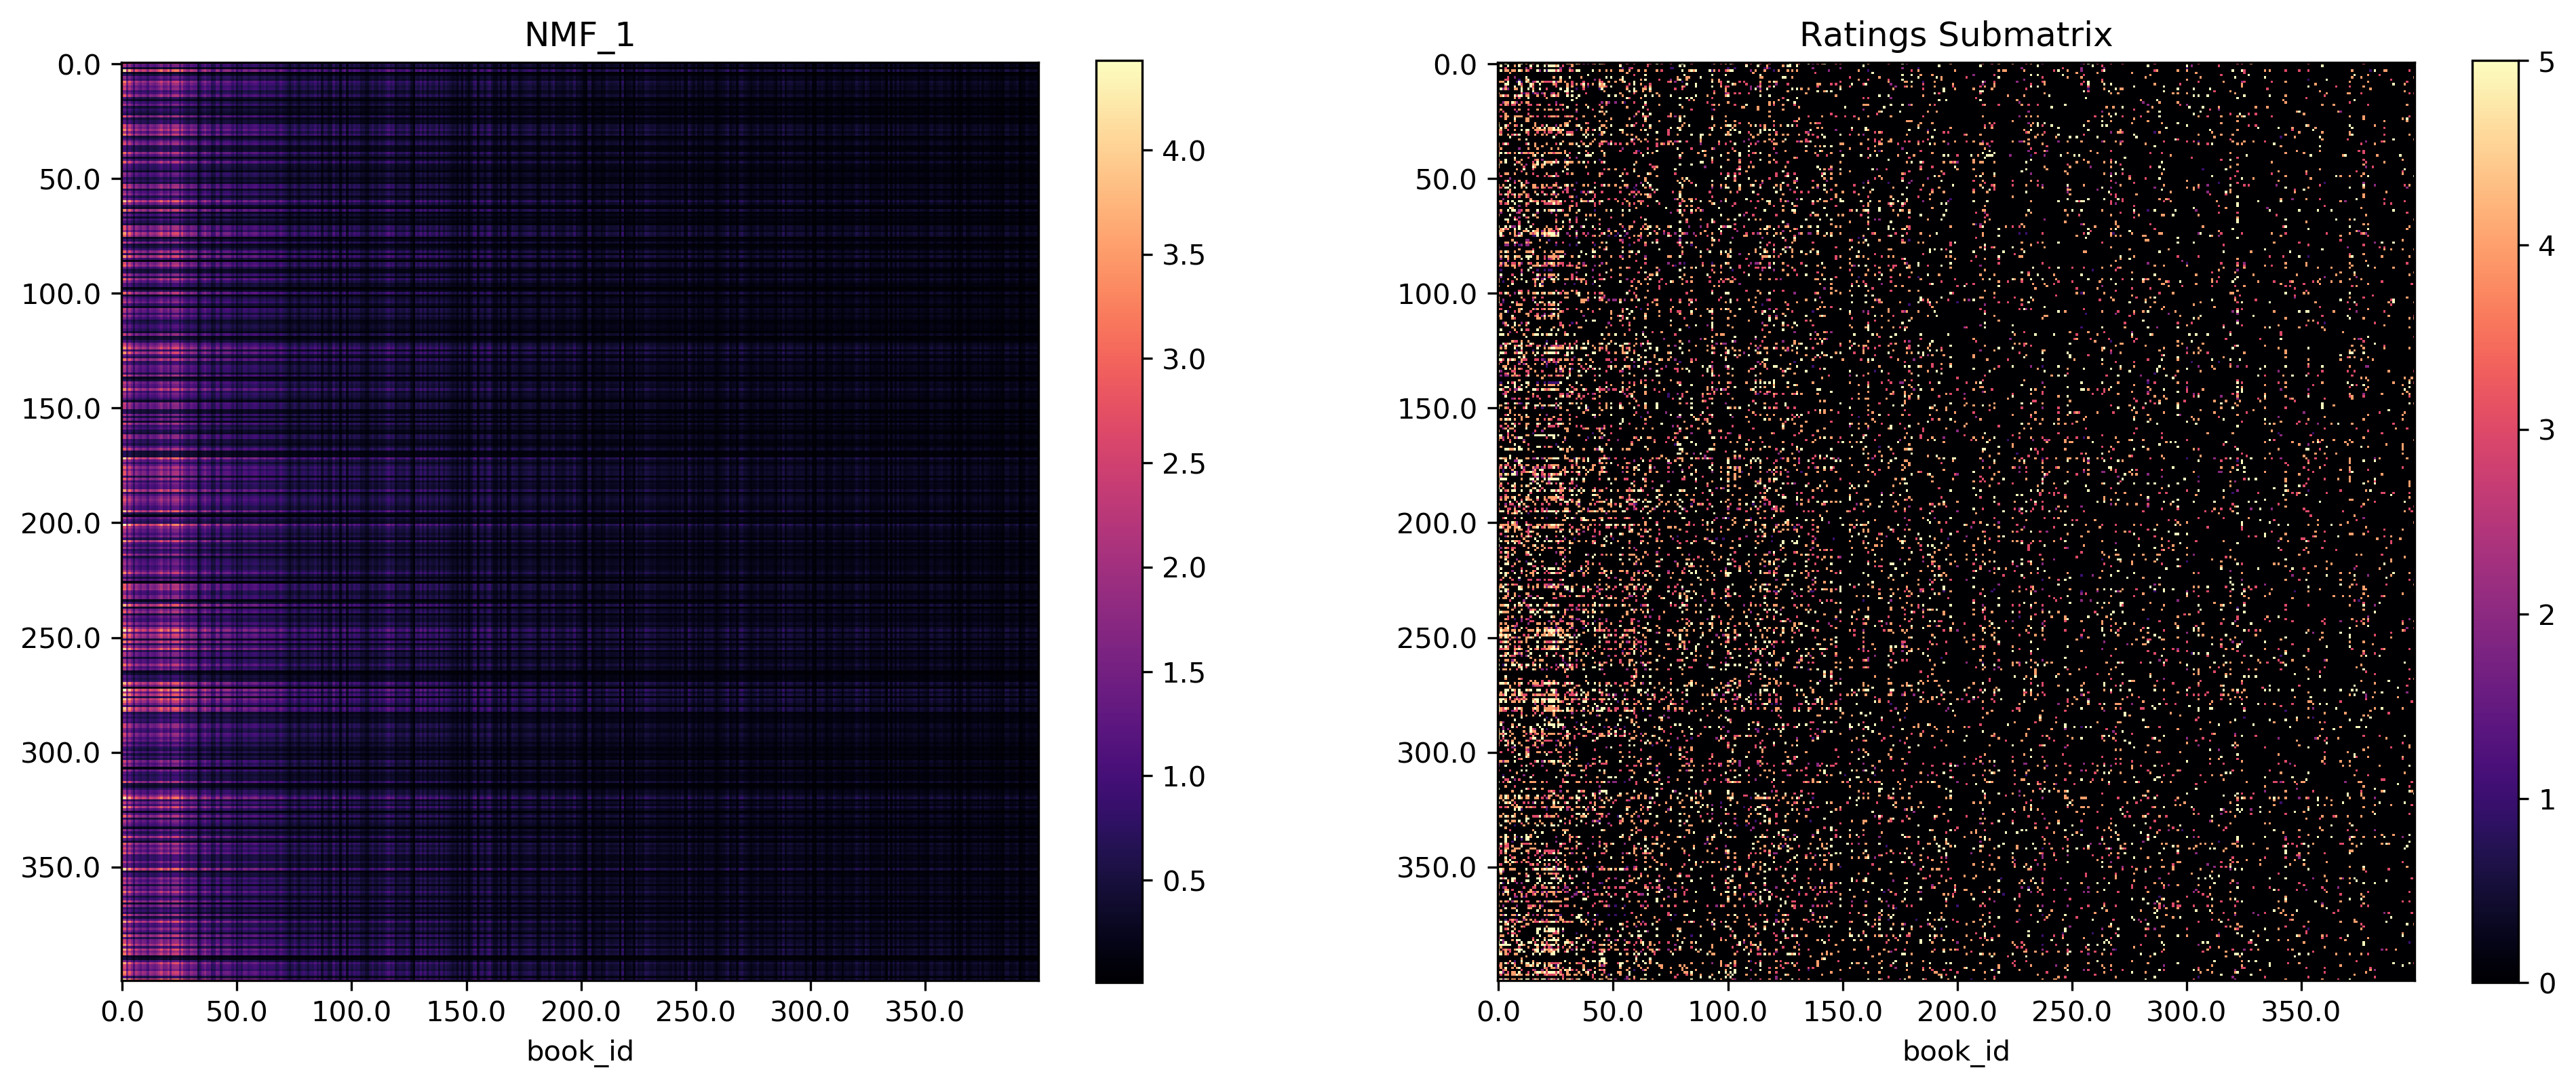
\includegraphics[width=\linewidth]{../image/goodreads-models/nmf-1-left.png}
%    \vspace{-30pt}
    \caption[NMF-1]{The matrix reconstruction compared aside the ratings matrix ($k=1$).}
     \label{fig:nmf-1}
\end{figure}


%______________________________________________________________________



%______________________________________________________________________




    \hypertarget{k>1}{%
\subsubsection{\texorpdfstring{\(k > 1\)}{k > 1}}\label{k>1}}

%
%\begin{wrapfigure}{r}{0.2\textwidth}
%    \centering
%    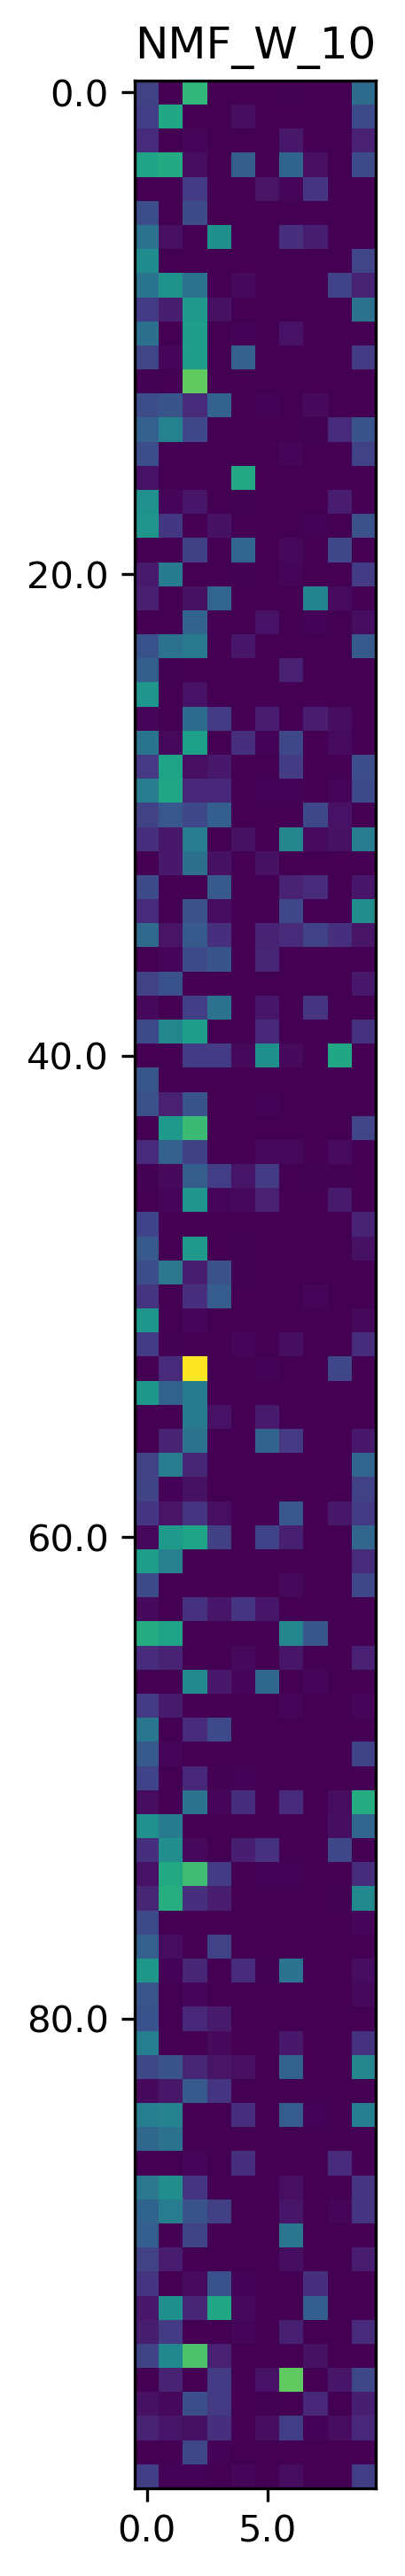
\includegraphics[width=0.12\textwidth]{../image/goodreads-models/nmf-W-10.png}
%    %\vspace{-30pt}
%    \caption[NMF-W-10]{%User preferences matrix.
%    }
%     \label{fig:nmf-W-10}
%\end{wrapfigure}

We have trained models for $k \in \{1, 10, 25, 50, 100, 250\}$. Lesser values of \(k\) give more
interpretable models, as we describe in section \ref{topic-extraction}, whereas greater values of \(k\) give more accurate
models, as in Figure \ref{fig:nmf-250-left-close}.
Upon viewing the matrices, we can also see that the matrix reconstruction becomes
finer and makes more `confident' recommendations for less popular books.
For lower values of $k$, the rows exhibit strong correlations between each other.
No regularization is applied to any of the models below, but we discuss and demonstrate the effects in section \ref{hyperparameters}.

\begin{figure}
    \centering
    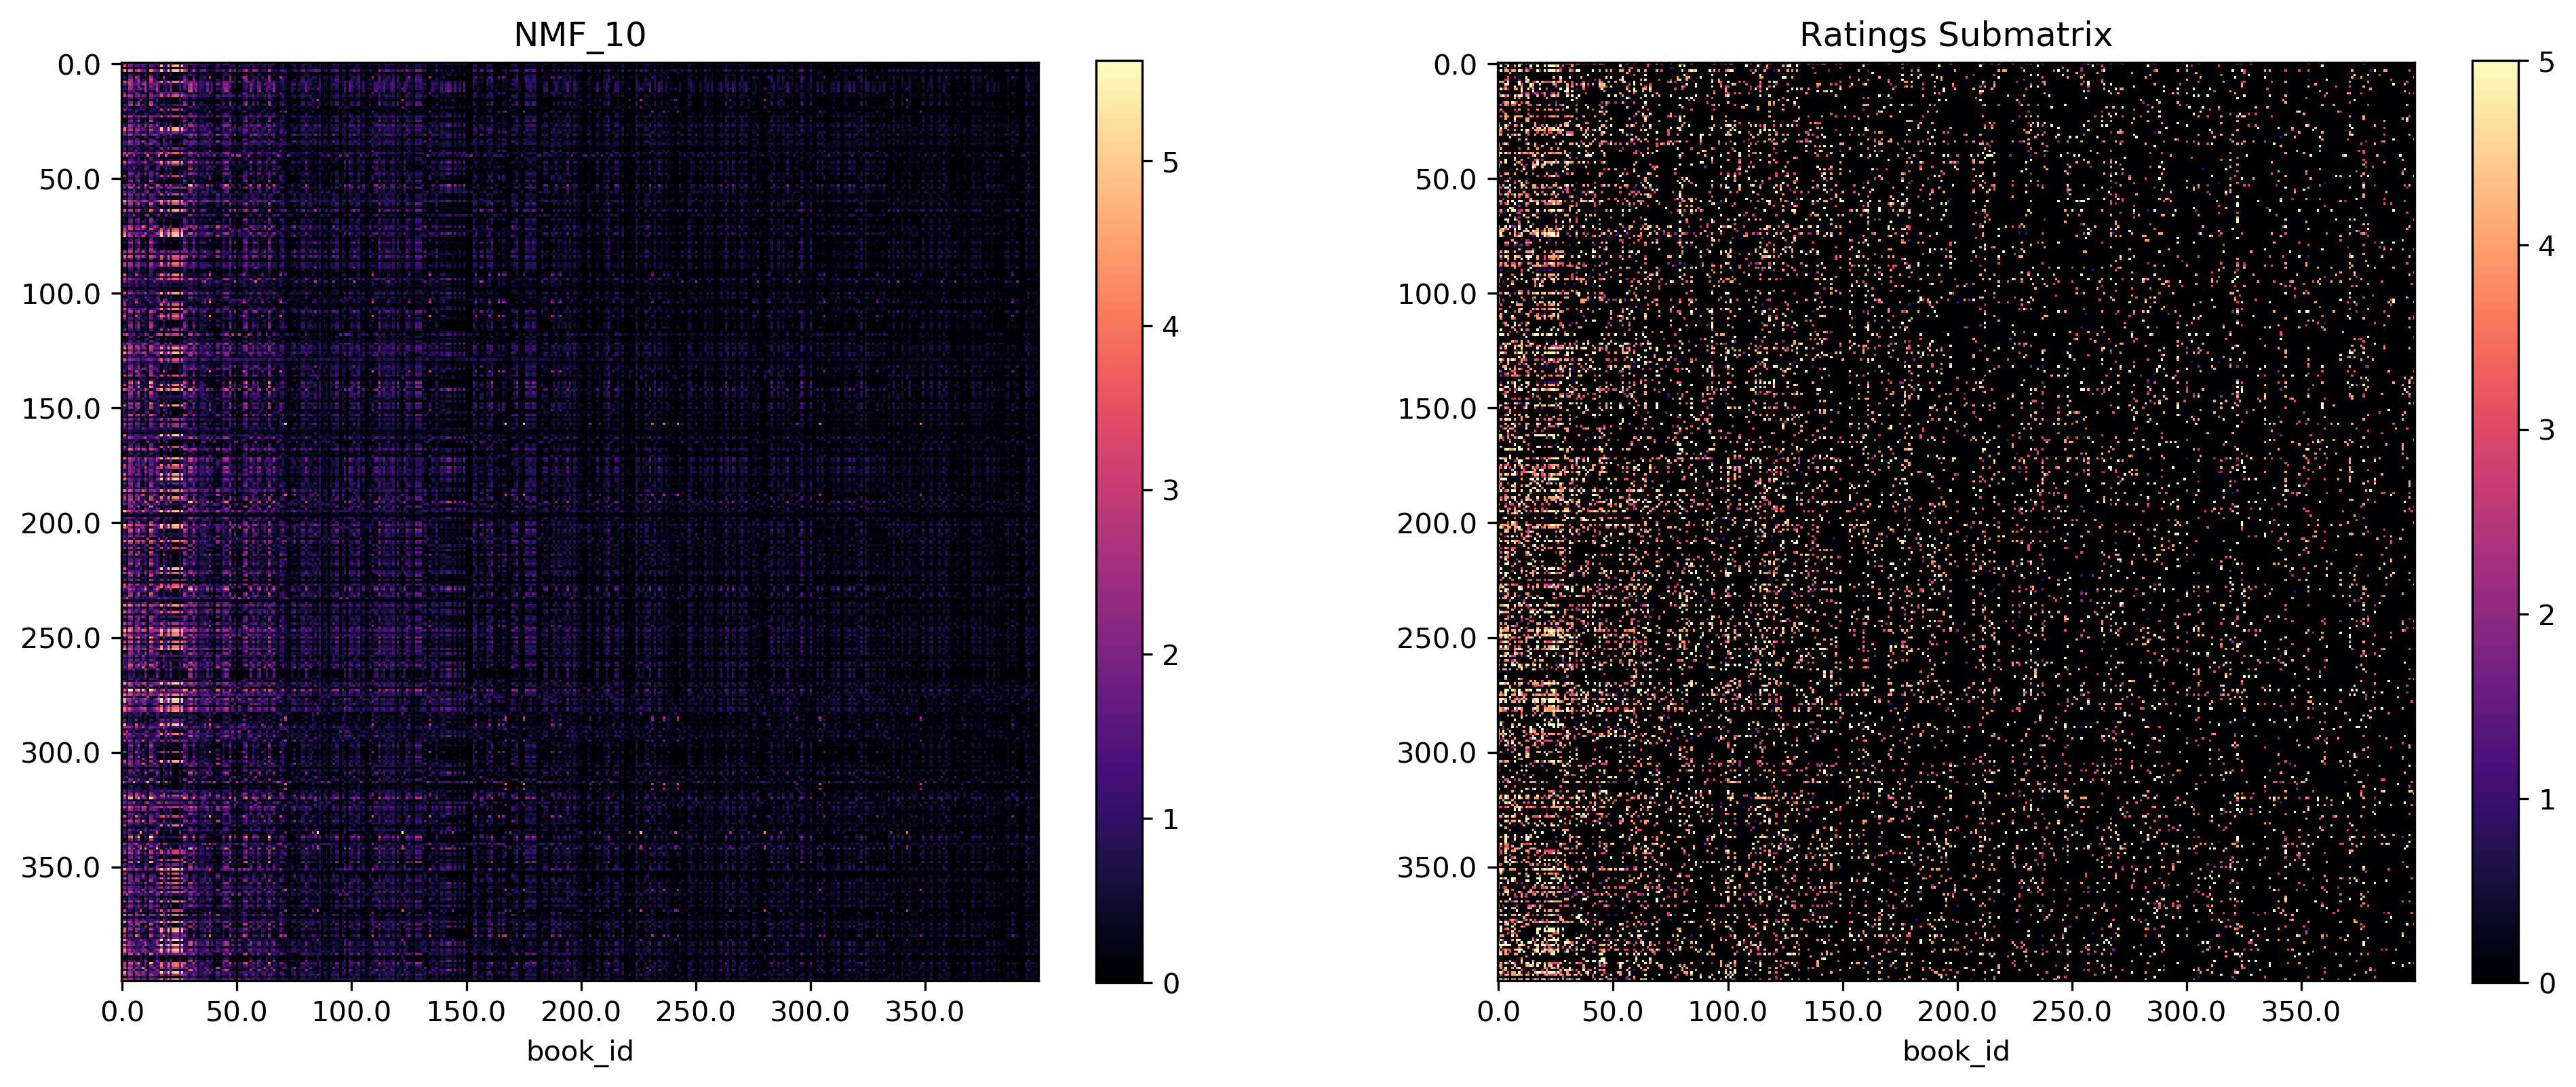
\includegraphics[width=\linewidth]{../image/goodreads-models/nmf-10-left.png}
%    \vspace{-30pt}
    \caption[NMF-10-Left]{Now the reconstruction clearly captures features of the ratings matrix.}
     \label{fig:nmf-10-left}
\end{figure}


\begin{figure}[p]
    \centering
    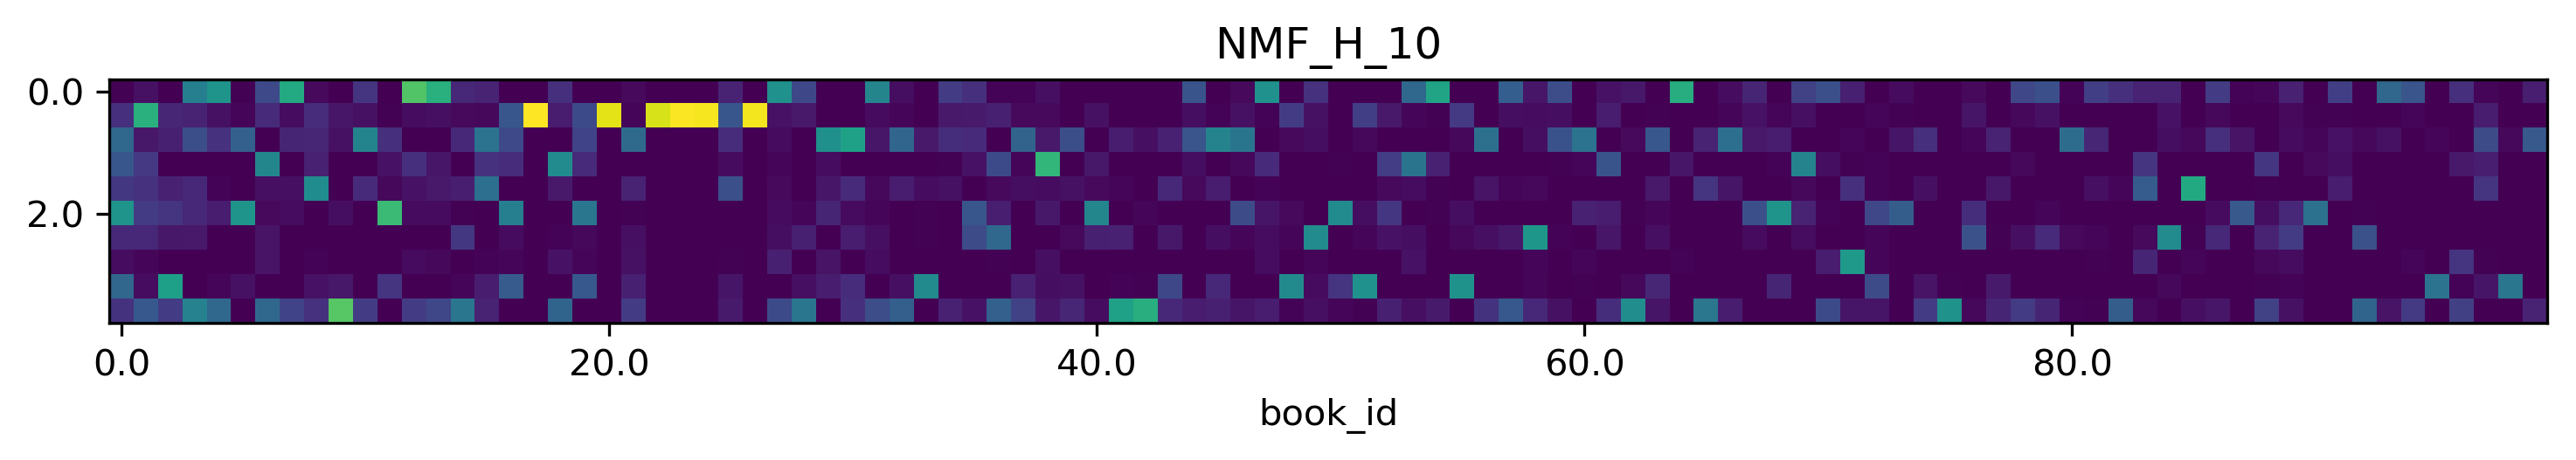
\includegraphics[width=\textwidth, trim=3cm 0cm 0cm 0cm, clip]{../image/goodreads-models/nmf-H-10.png}
%    \vspace{-30pt}
    \caption[NMF-H-10]{The size of the $k=10$ model is 5MB.}
     \label{fig:nmf-H-10}
\end{figure}



\begin{figure}[p]
    \centering
    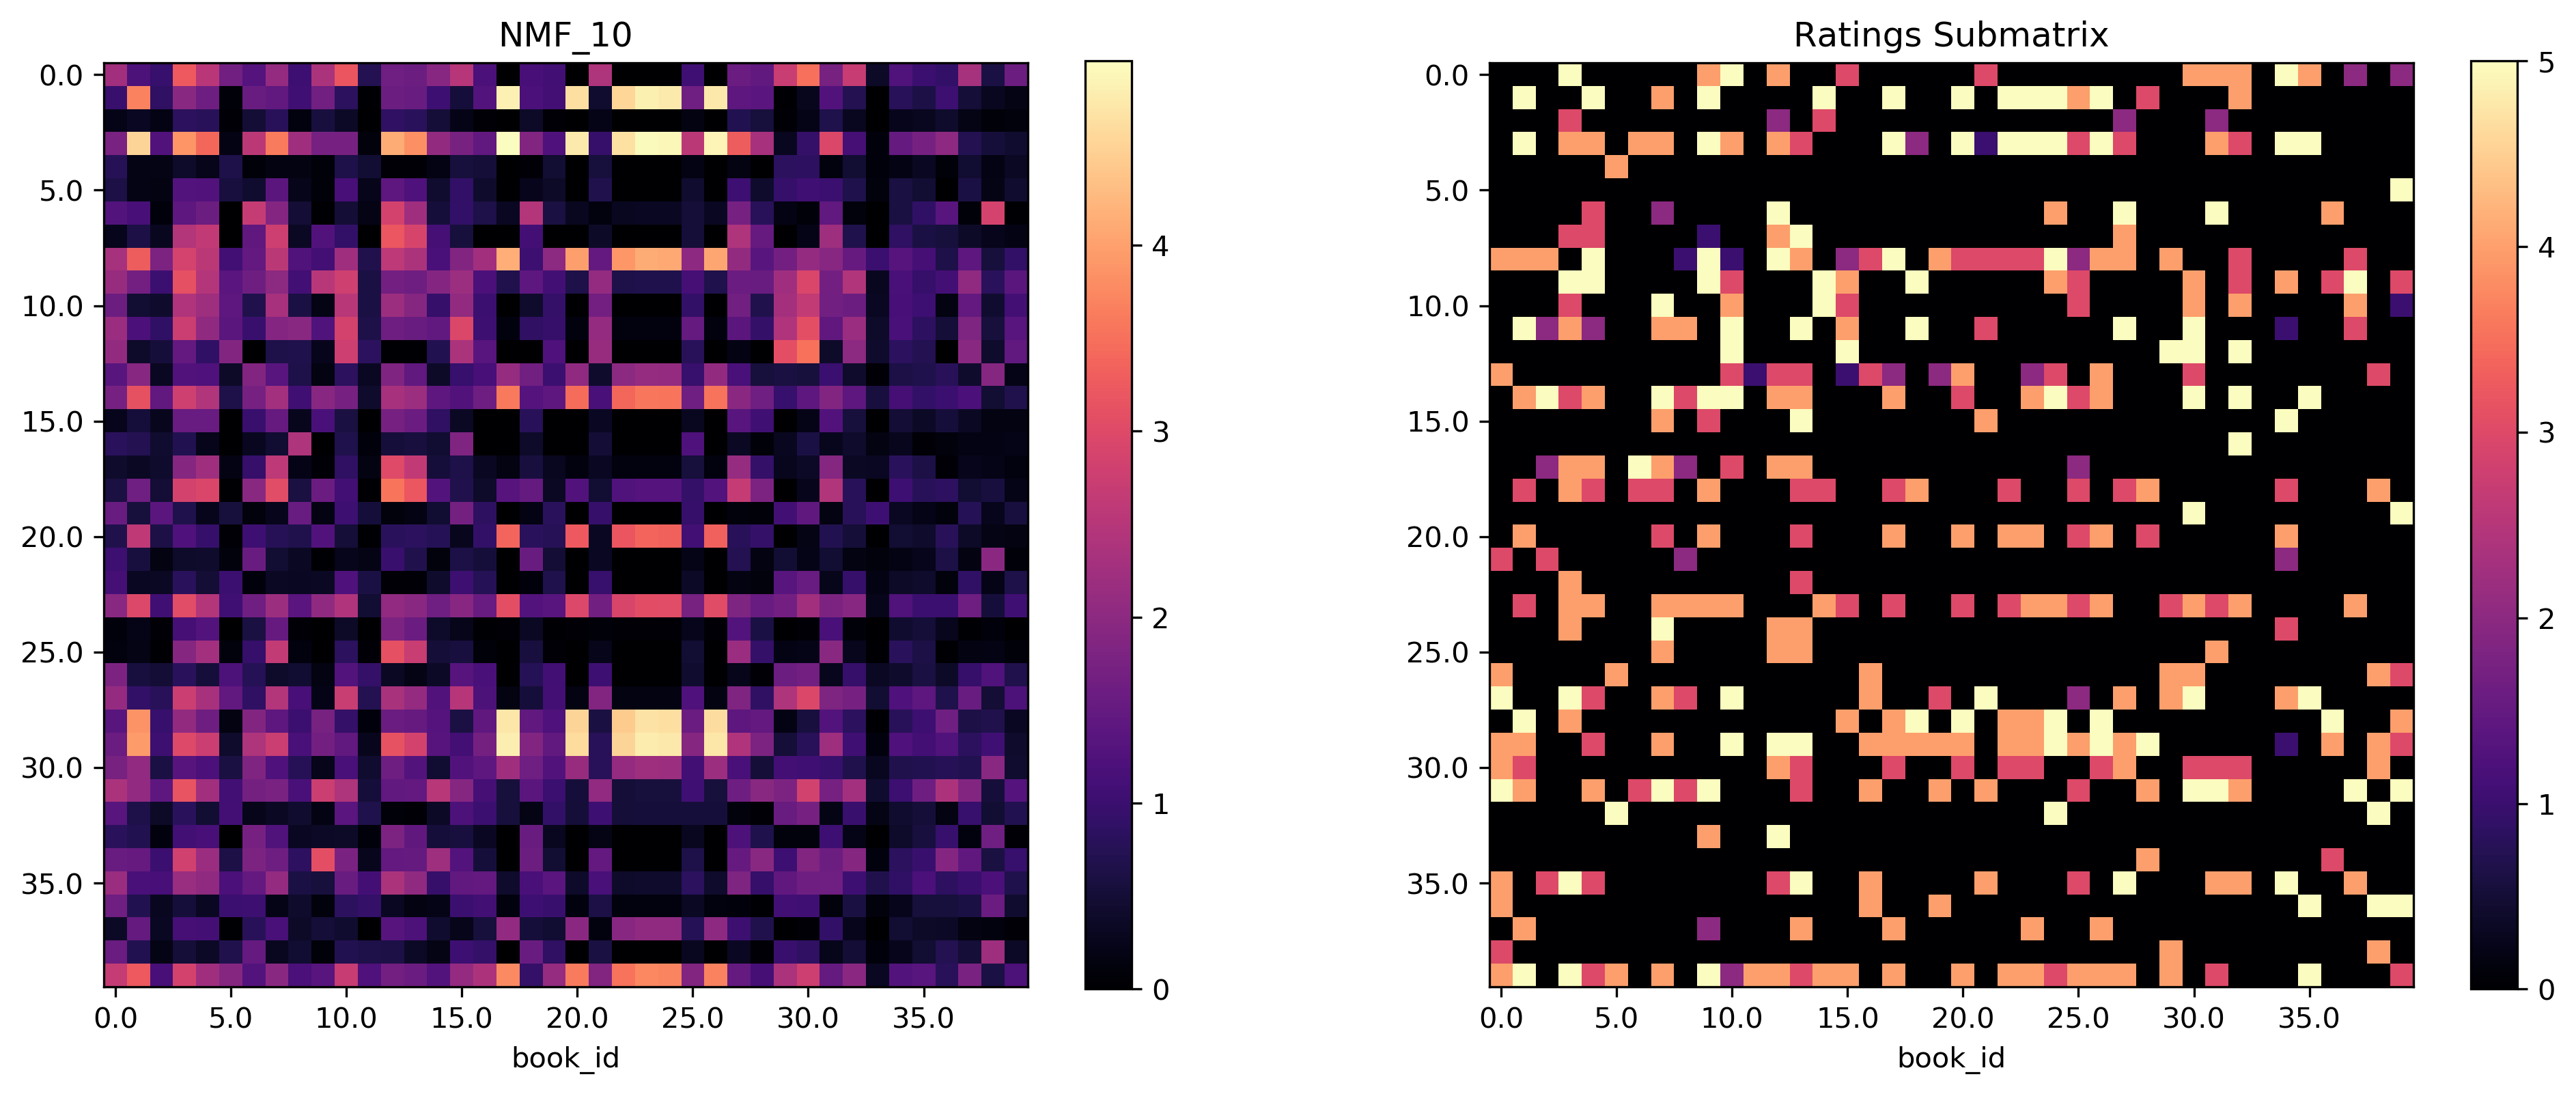
\includegraphics[width=\linewidth]{../image/goodreads-models/nmf-10-left-close.png}
%    \vspace{-30pt}
    \caption[NMF-10-Left-Close]{Looking closer, we can see that the reconstruction fills in entries with no rating in the ratings matrix.}
     \label{fig:nmf-10-left-close}
\end{figure}

\begin{figure}[p]
    \centering
    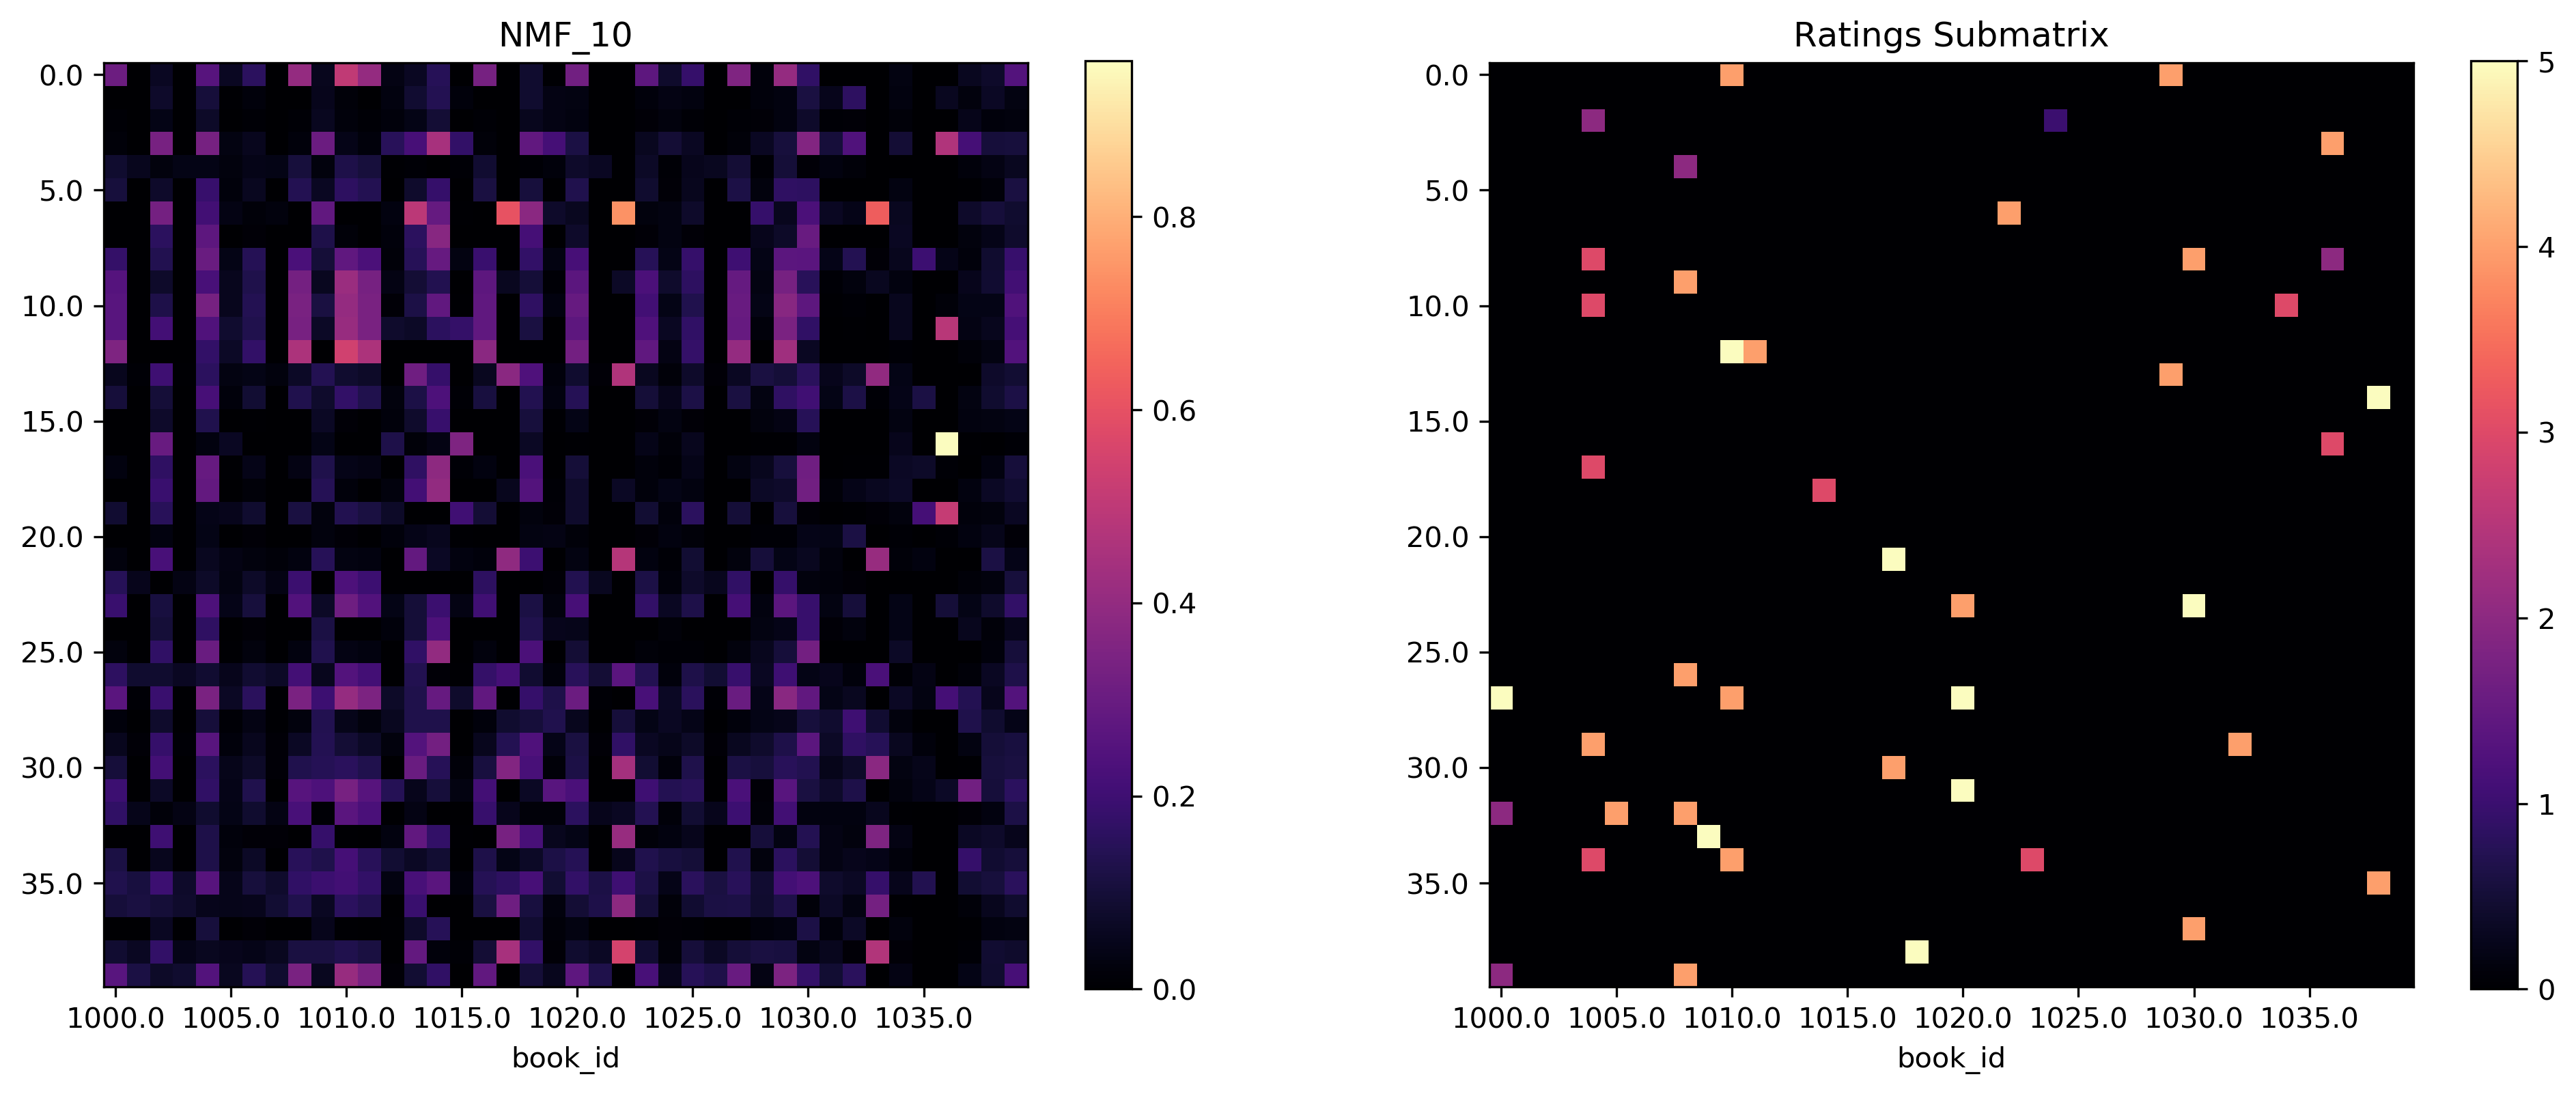
\includegraphics[width=\linewidth]{../image/goodreads-models/nmf-10-left-center-close.png}
%    \vspace{-30pt}
    \caption[NMF-10-Left-Center-Close]{Moving 1000 columns to the right, we see a sparser portion of the matrix.}
     \label{fig:nmf-10-left}
\end{figure}


\begin{figure}[p]
    \centering
    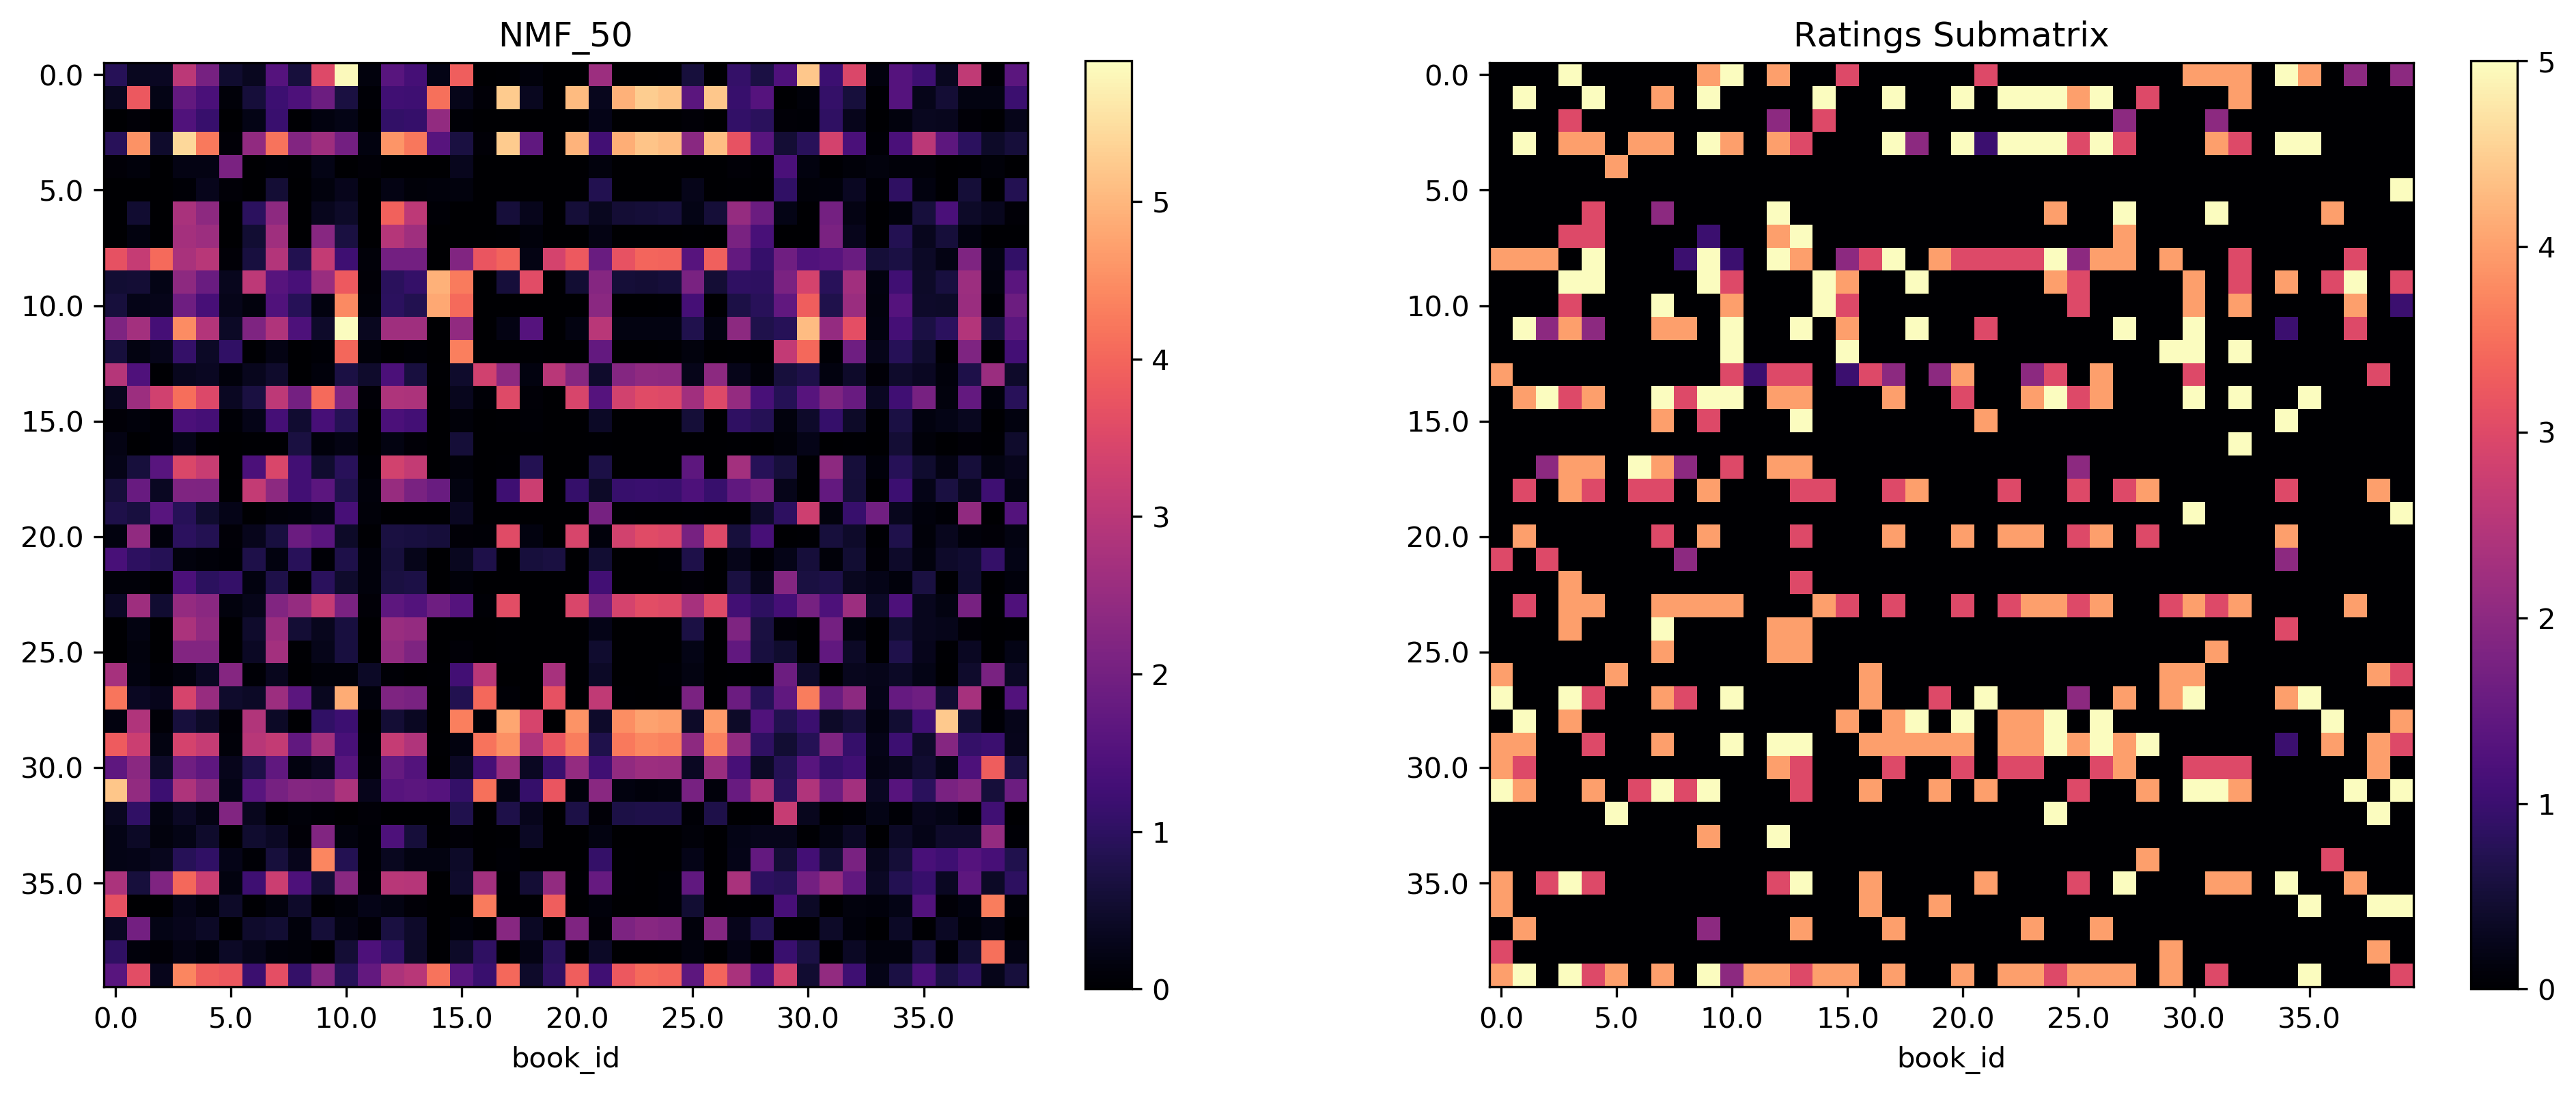
\includegraphics[width=\linewidth]{../image/goodreads-models/nmf-50-left-close.png}
%    \vspace{-30pt}
    \caption[NMF-50-Left-Close]{Visually, at $k=50$, we see the rows are less correlated;
    each row is a linear combination of 50 vectors rather than 10 as in the $k=10$ case.}
     \label{fig:nmf-50-left-close}
\end{figure}



\begin{figure}[p]
    \centering
    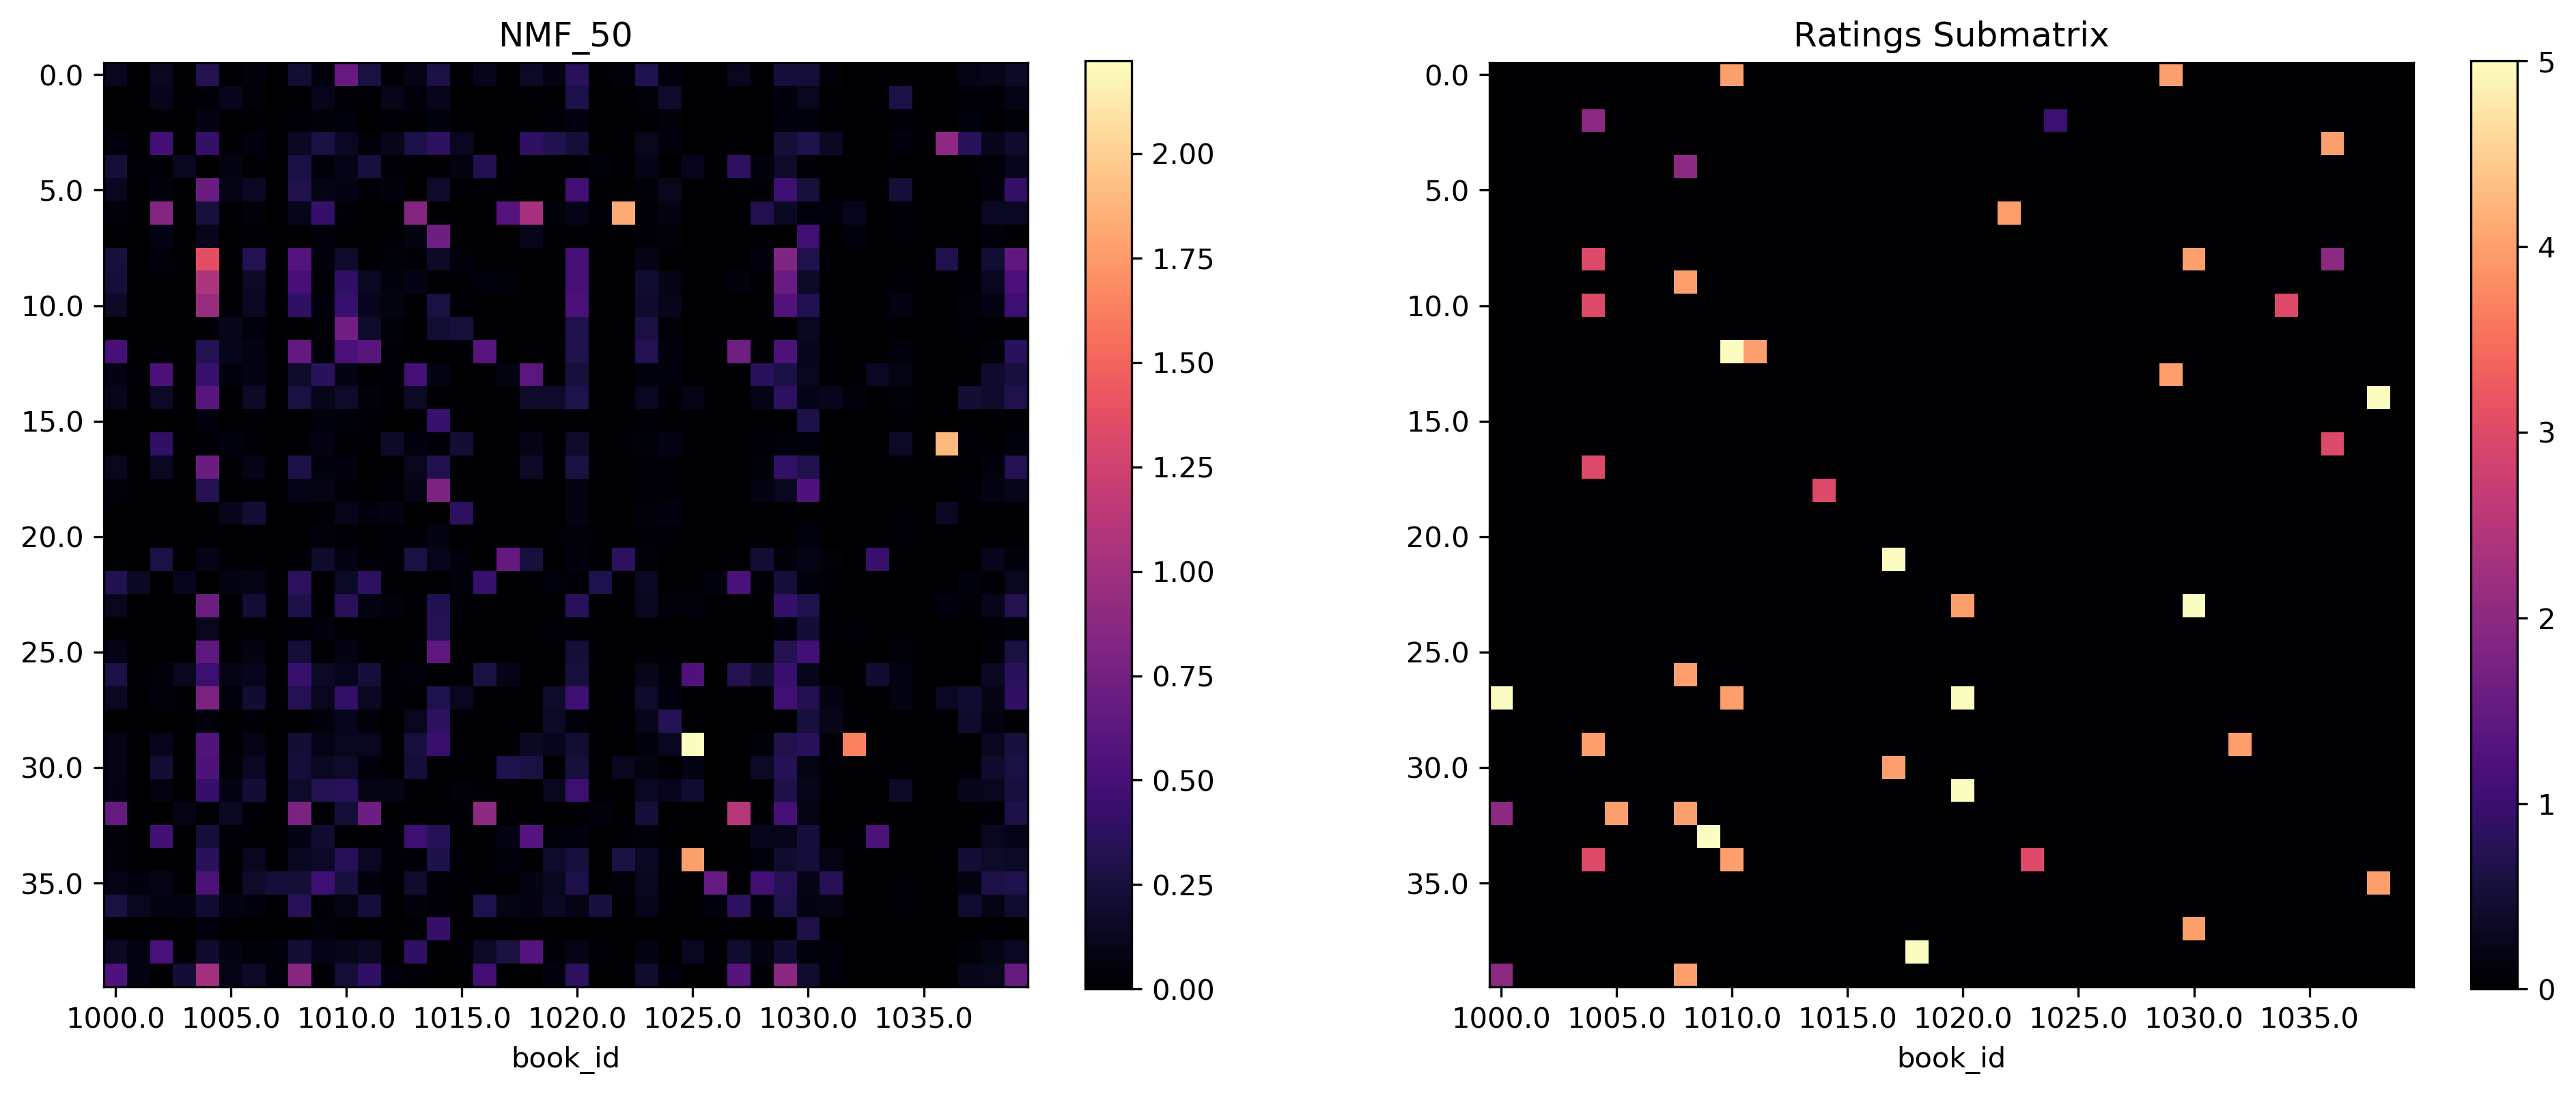
\includegraphics[width=\linewidth]{../image/goodreads-models/nmf-50-left-center-close.png}
%    \vspace{-30pt}
    \caption[NMF-50-Left-Center-Close]{For $k=50$ the correlations in sparser areas of the 
    matrix reconstruction are stronger than for $k=10$.}
     \label{fig:nmf-50-left-center-close}
\end{figure}



%\begin{wrapfigure}{r}{0.2\textwidth}
%  %  \centering
%    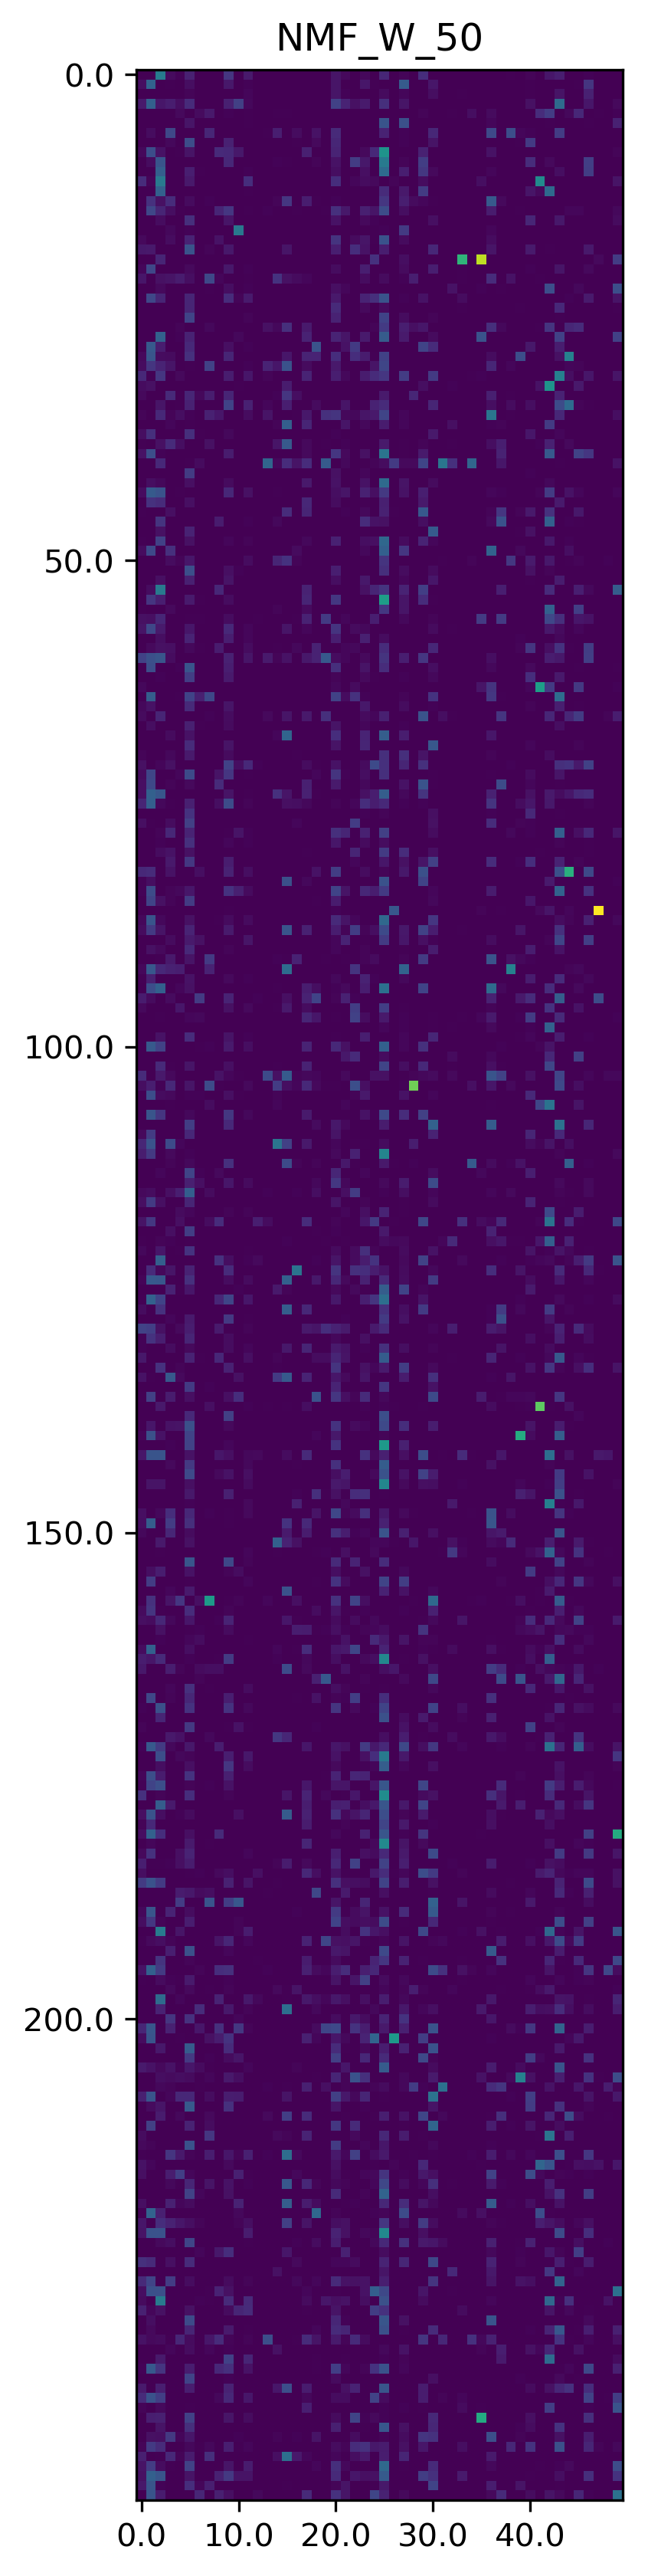
\includegraphics[height=\textheight]{../image/goodreads-models/nmf-W-50.png}
%%    \vspace{-30pt}
%%    \caption[NMF-W-50]{A portion of the user preferences matrix.}
%     \label{fig:nmf-W-50}
%\end{wrapfigure}

\begin{figure}[p]
  %  \centering
    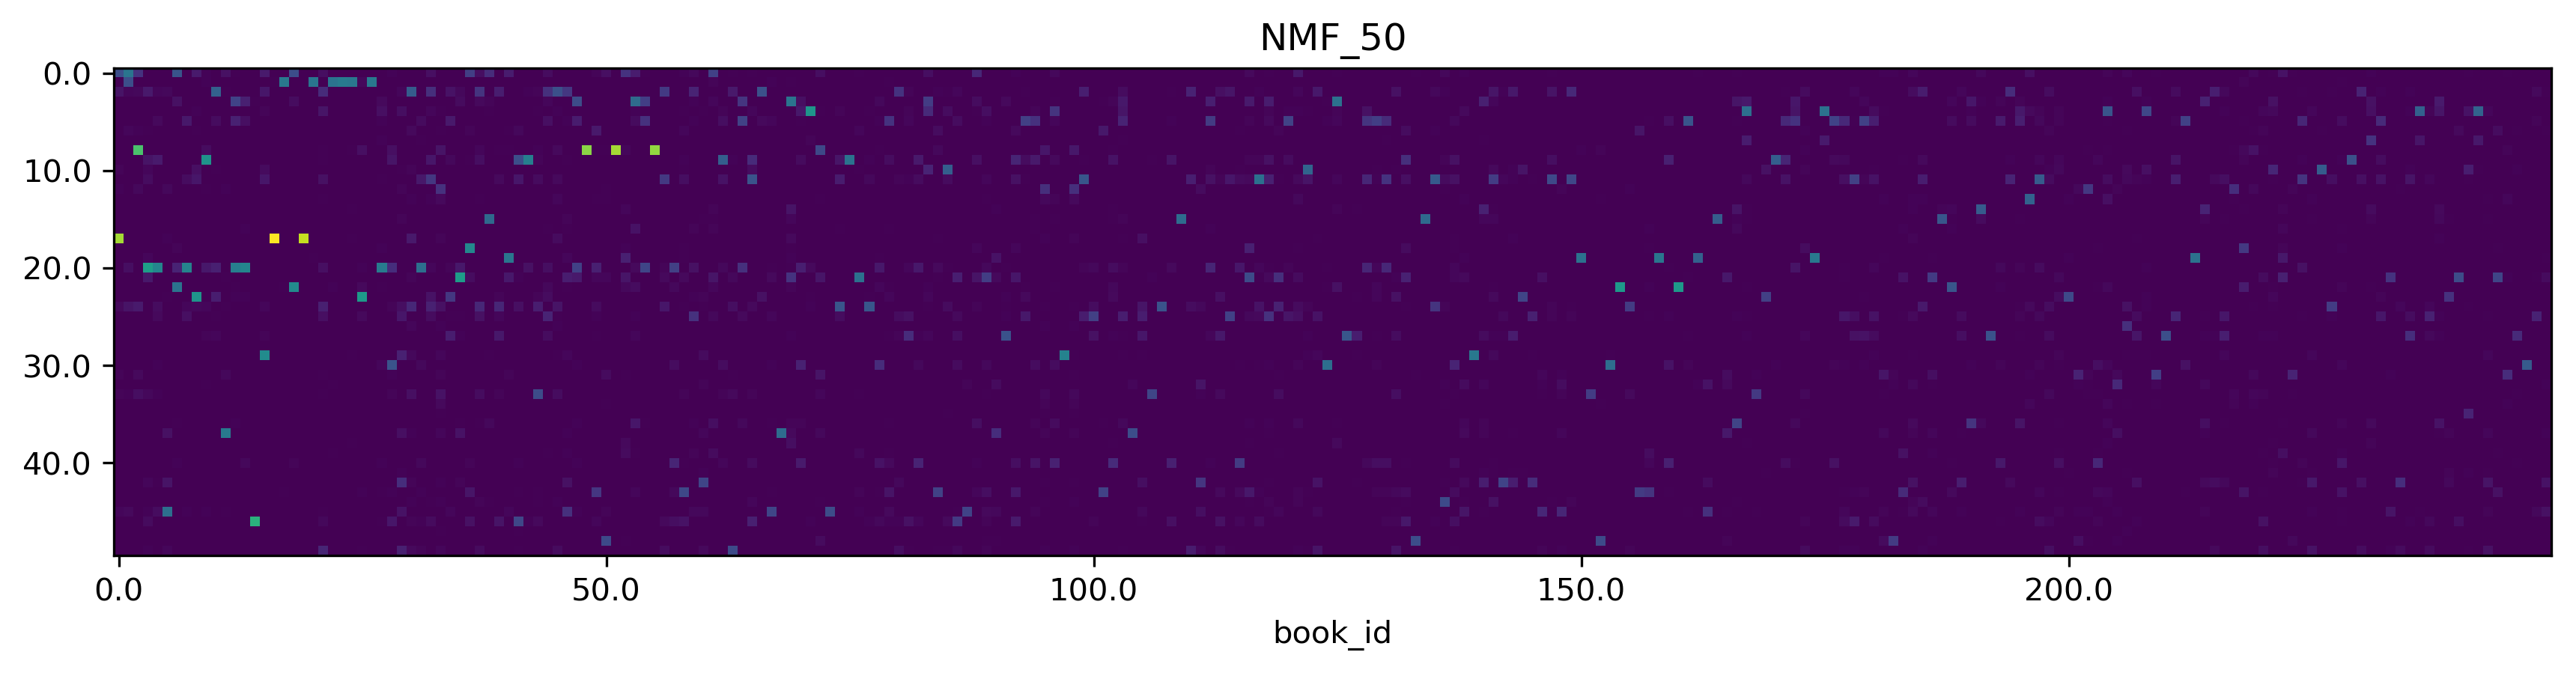
\includegraphics[width=\linewidth, trim=3cm 0cm 0cm 0cm, clip]{../image/goodreads-models/nmf-H-50.png}
%    \vspace{-30pt}
    \caption[NMF-H-50]{The size of the $k=50$ model is 25MB. The first few hundred columns of $H$ are shown.}
     \label{fig:nmf-H-50}
\end{figure}


\begin{figure}[p]
  %  \centering
    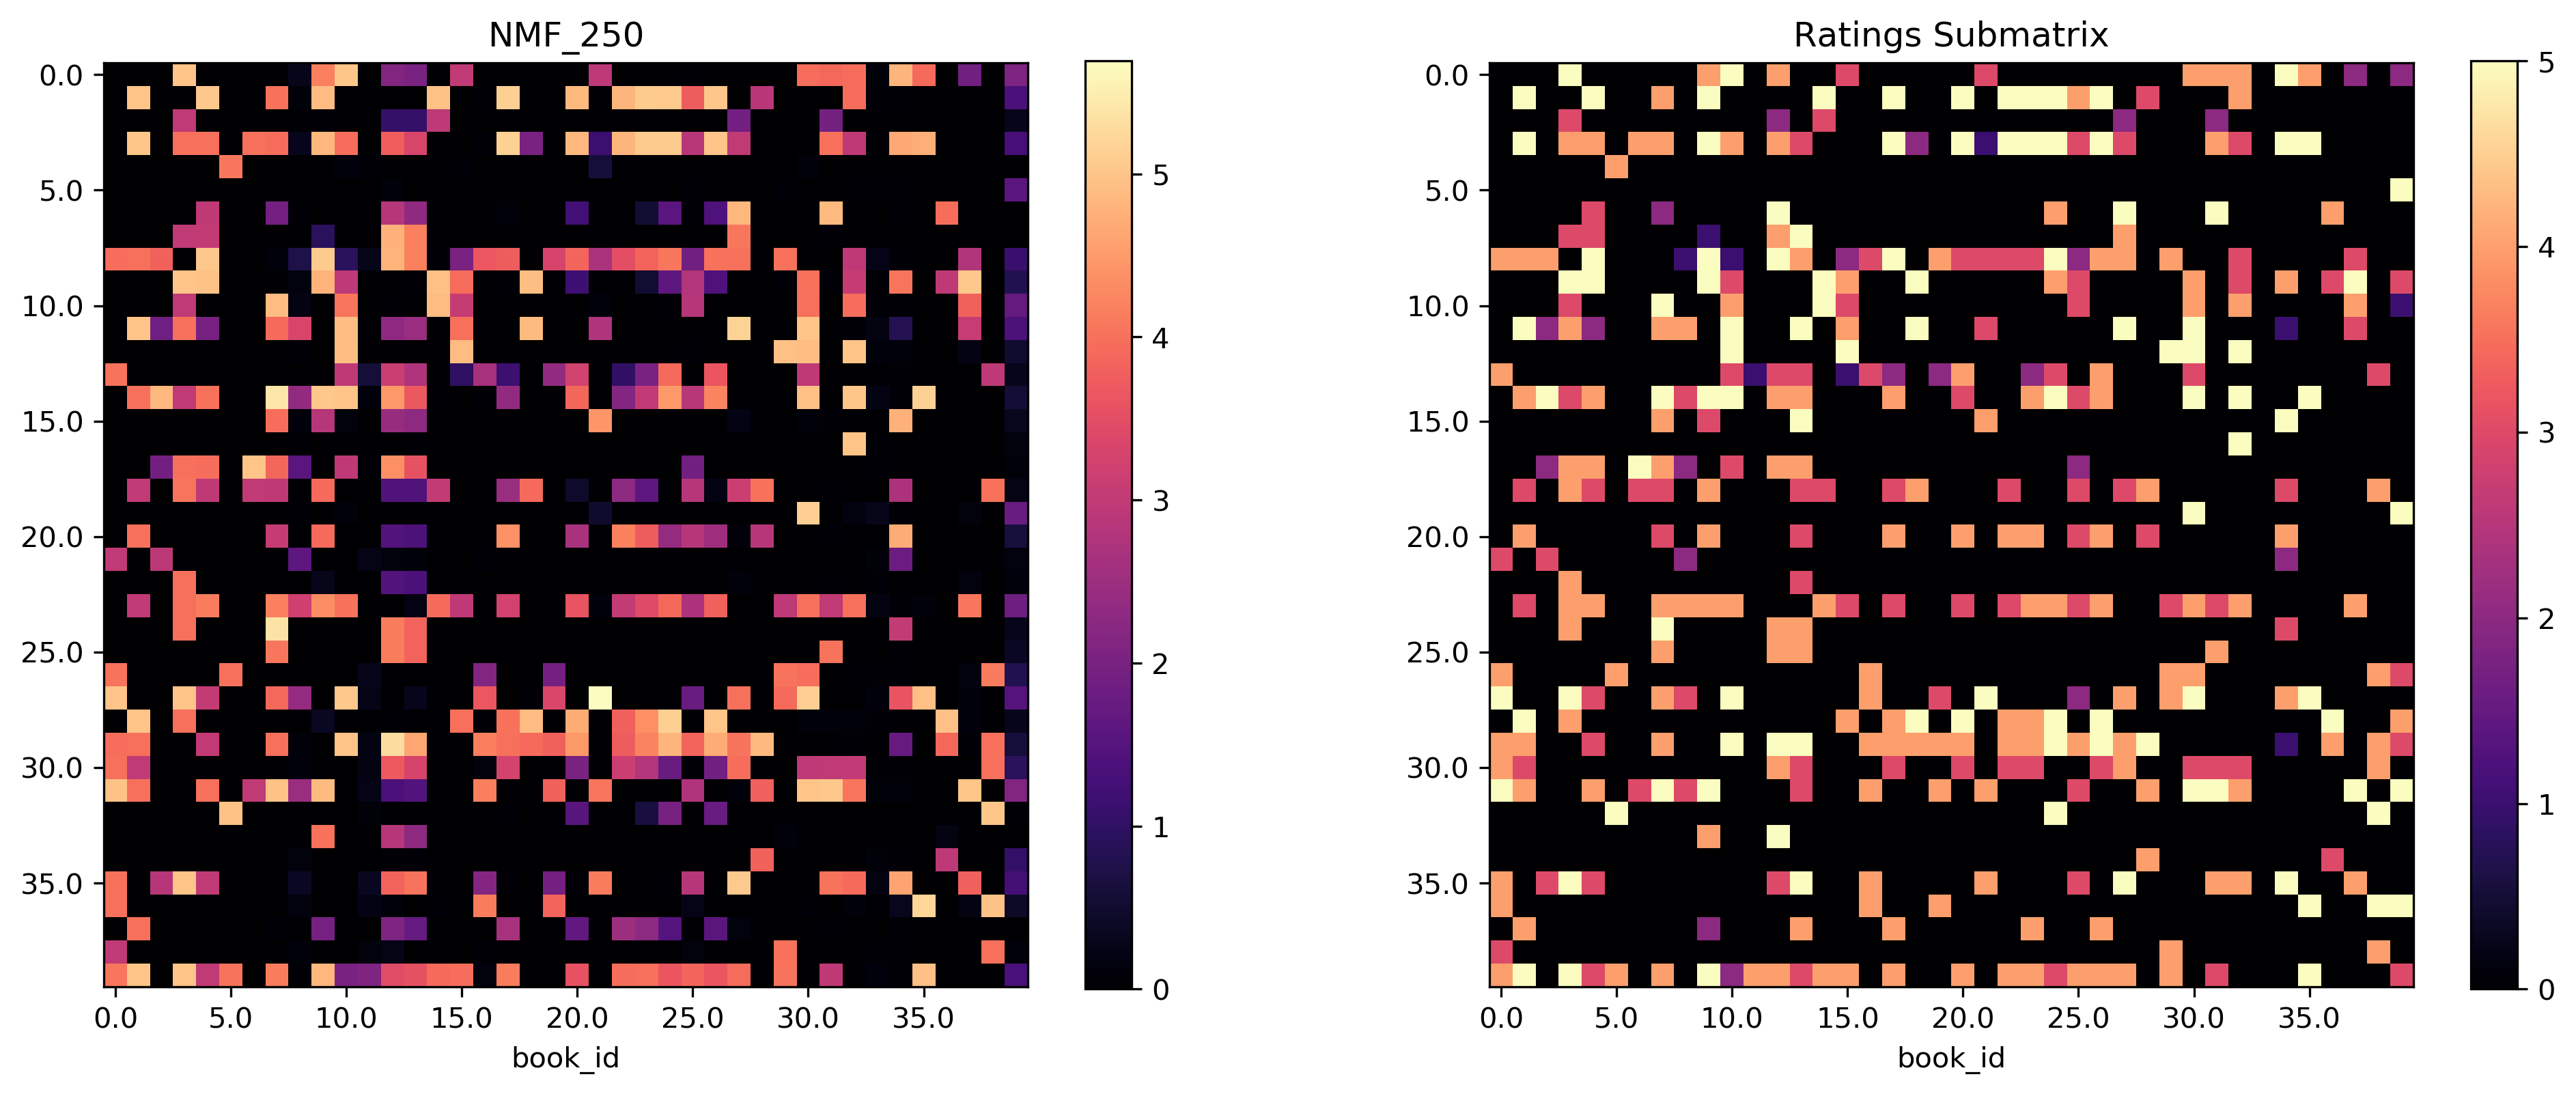
\includegraphics[width=\linewidth]{../image/goodreads-models/nmf-250-left-close.png}
%    \vspace{-30pt}
    \caption[NMF-250-Left-Close]{$k=250$ uses roughly 125MB. While in the upper left $400 \times 400$, there are some points such that
    the reconstruction value is as great as 14, it is notable that none of the values shown is greater than 6.}
     \label{fig:nmf-250-left-close}
\end{figure}



\begin{figure}[p]
  %  \centering
    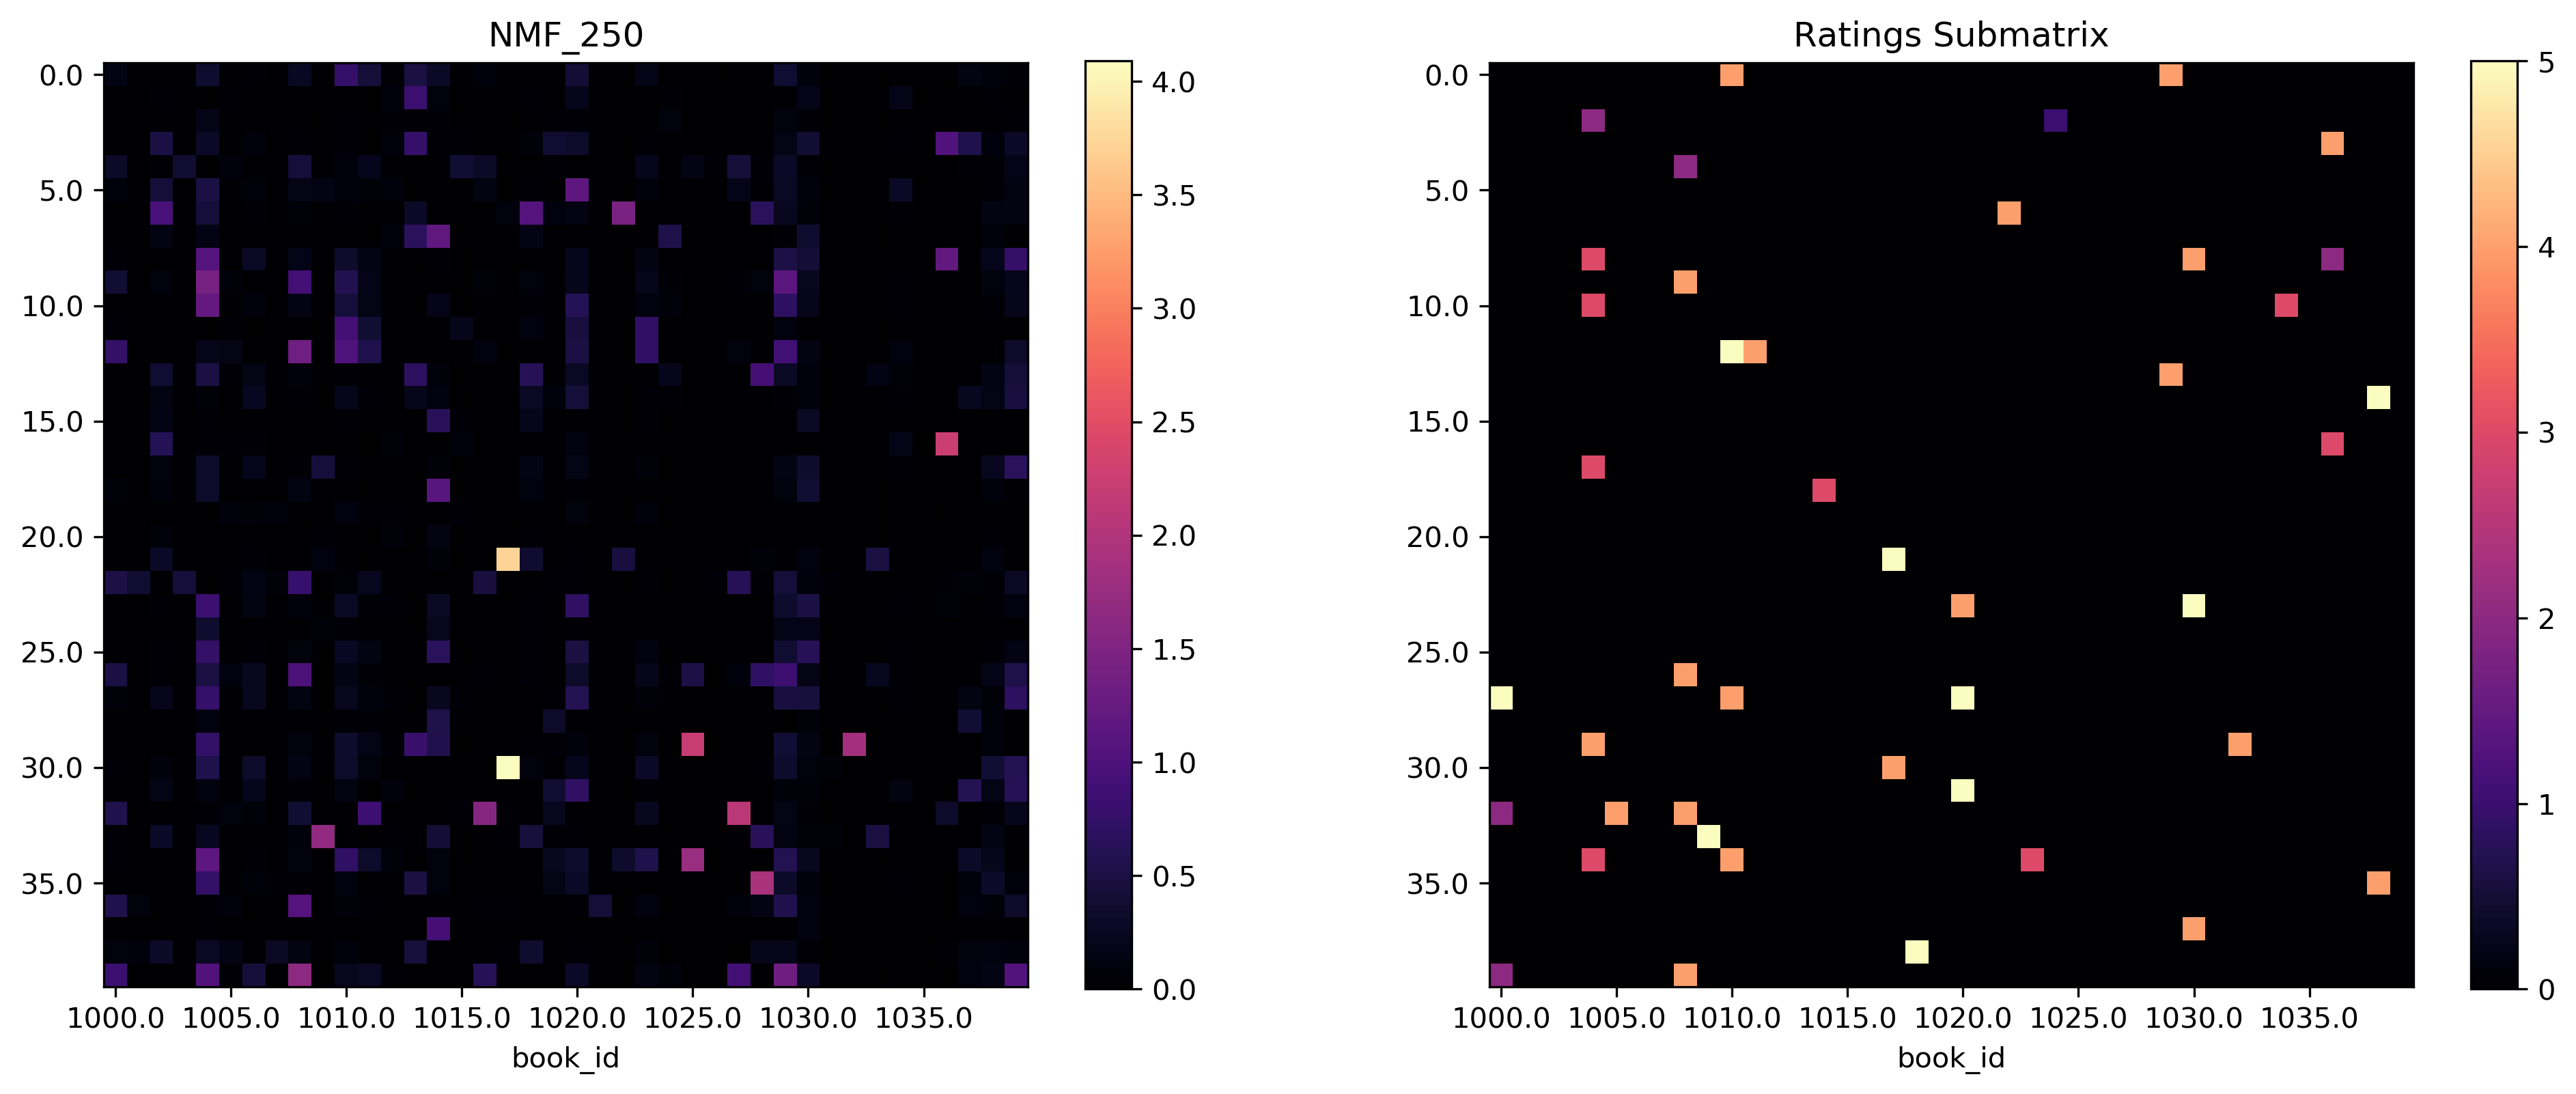
\includegraphics[width=\linewidth]{../image/goodreads-models/nmf-250-left-center-close.png}
%    \vspace{-30pt}
    \caption[NMF-250-Left-center-Close]{For $k=250$ the correlations in sparser areas of the 
    matrix reconstruction are considerably greater than in $k=50$ or $k=10$.}
     \label{fig:nmf-250-left-center-close}
\end{figure}


\begin{figure}[h]
  %  \centering
    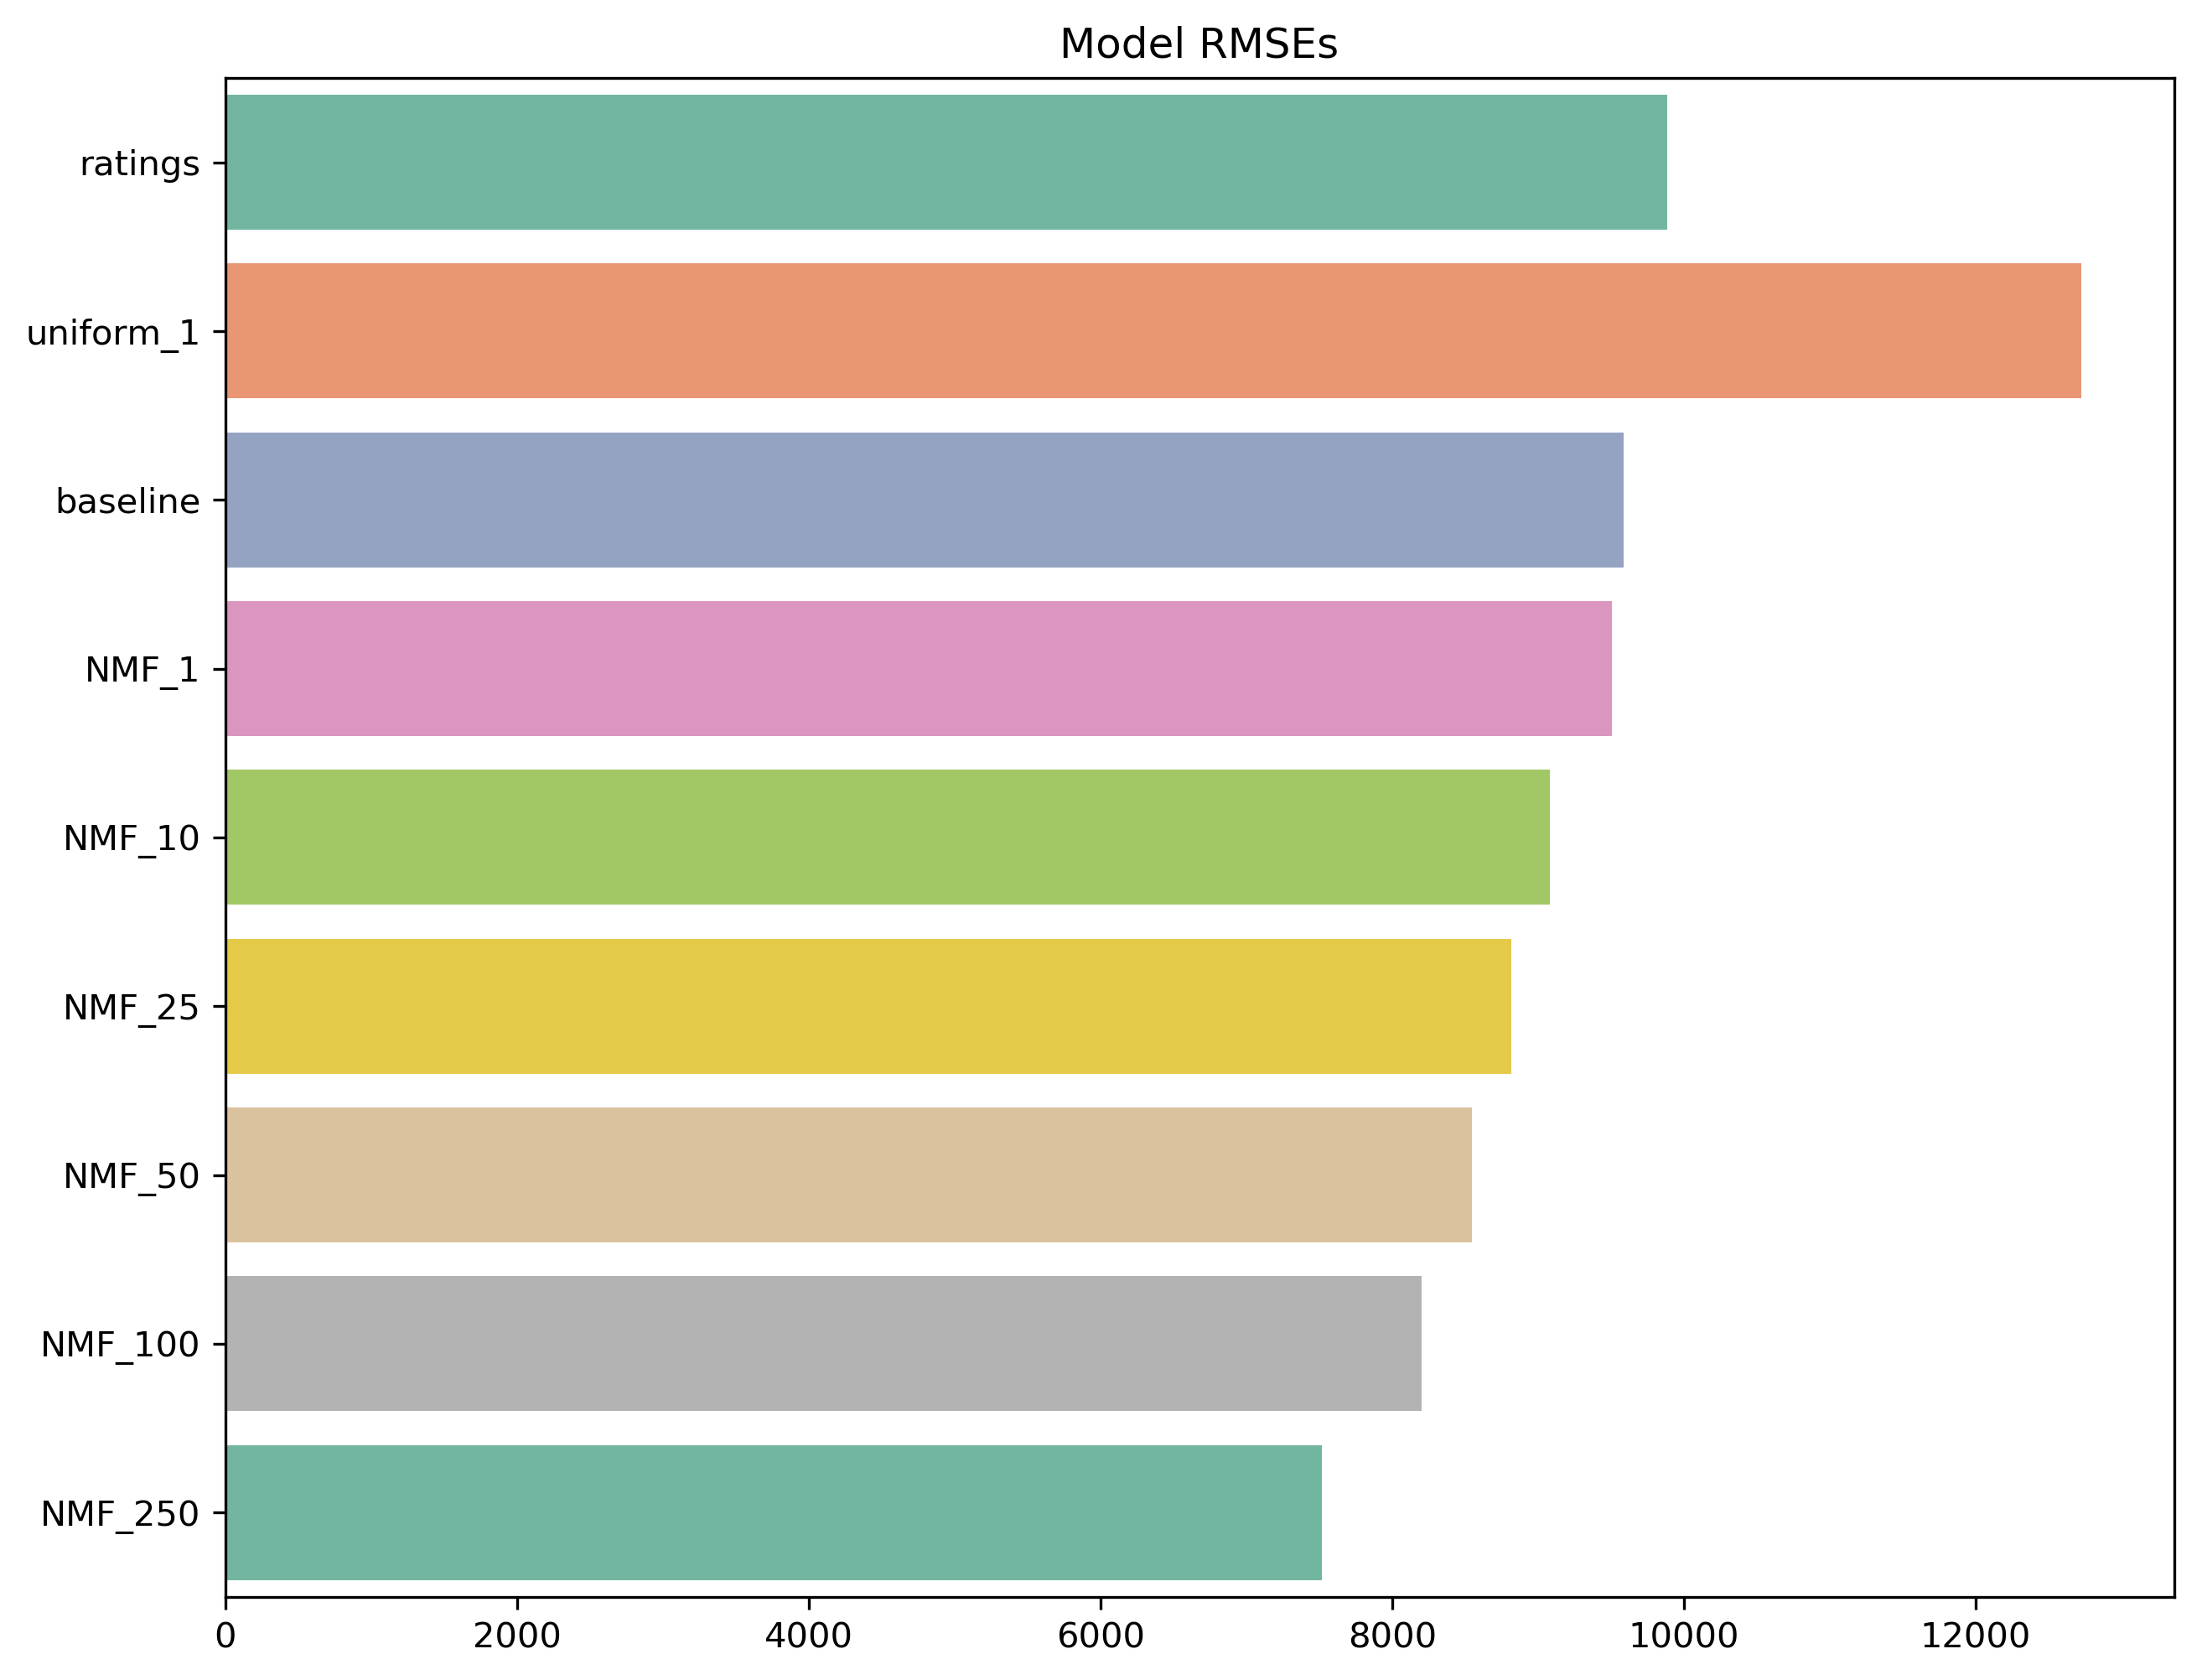
\includegraphics[width=\linewidth]{../image/goodreads-models/model-rmses.png}
%    \vspace{-30pt}
    \caption[RMSE Comparison]{The $k=250$ model factorization requires roughly 45 minutes to compute on Kaggle's platform;
    it may be reasonable to consider larger factorizations for recommendations.}
     \label{fig:rmse}
\end{figure}


%______________________________________________________________________





\begin{figure}[t]
  %  \centering
    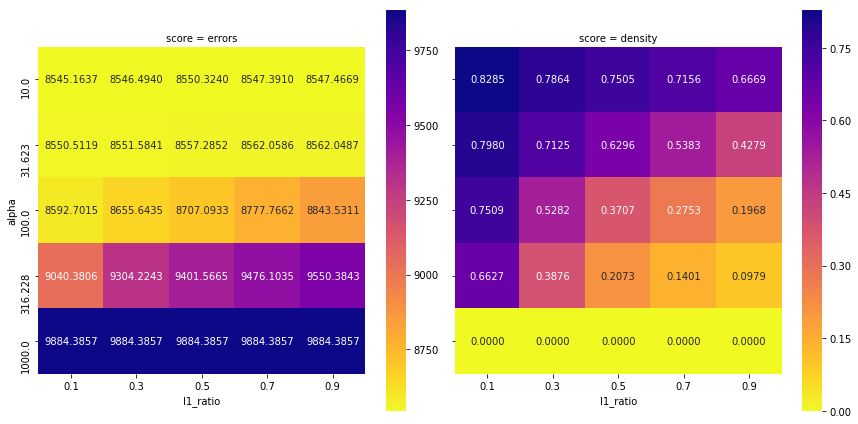
\includegraphics[width=\linewidth]{../image/goodreads-l1-and-l2-regularization/output_18_0.png}
%    \vspace{-30pt}
    \caption[$L1$- and $L2$-regularization]{$k=50$. We can see an accuracy/sparsity trade-off between $L1$- and $L2$-regularization.}
     \label{fig:regularization}
\end{figure}




    \hypertarget{hyperparameters}{%
\subsection{Hyperparameters}\label{hyperparameters}}



The hyperparameters of \href{}{\texttt{sklearn.decomposition.NMF}} are similar to those of 
\href{https://scikit-learn.org/stable/modules/generated/sklearn.linear_model.ElasticNet.html#sklearn.linear_model.ElasticNet}{\texttt{sklearn.linear\_models.ElasticNet}}
in that we can tune the magnitude $\alpha := \lambda_1 + \lambda_2$ and the \texttt{l1\_ratio}, $\rho = \frac{\lambda_1}{\lambda_1 + \lambda_2}$,
where $\lambda_1$ and $\lambda_2$ are as in equation \eqref{eq:reg-loss-fcn}.
Figure \ref{fig:regularization} shows the effects of $L1$- and $L2$-regularization for $k=50$.
$L2$-regularization does not seem to help RMSE much except for some of the largest values of $k$ we examine, and even then only marginally,
so none of the models above include any $L2$-regularization.

$L1$-regularization is useful in controlling sparsity.
This lowers RMSE but could still be advantageous as it 'zeros out' entries with very low correlation which would not be a factor in our recommendations anyway.
A dense matrix of size $n_u \times n_b$ is a few GB, which is quite tractable, so we do not apply any $L1$-regularization to the models above.
In a more realistic situation, we may expect $n_b, n_u \approx 10^6$ rather than $n_b, n_u \approx 10^4$,
so that a model with sparse reconstructions may be advantageous at a deployment or engineering phase.

%______________________________________________________________________





%______________________________________________________________________
%______________________________________________________________________
%______________________________________________________________________
%______________________________________________________________________
%______________________________________________________________________

\newpage

    \hypertarget{topic-extraction}{%
\section{Topic Extraction \& Recommendations}\label{topic-extraction}}


%______________________________________________________________________
\begin{wraptable}{r}{0.40\textwidth}
\vspace{-10pt}
\centering
  \begin{tabular}{lr}
\toprule
{} &    9 \\
topic\_name              &      \\
\midrule
Harry Potter            & 0.29 \\
Modern Classics         & 0.22 \\
Fiction                 & 0.22 \\
Twilight \& Fifty Shades & 0.12 \\
Austen \& Brontës        & 0.06 \\
Thrillers               & 0.02 \\
Stephen King            & 0.00 \\
Children's              & 0.00 \\
Young Adult             & 0.00 \\
Fantasy \& Sci-Fi        & 0.00 \\
\bottomrule
\end{tabular}

  \caption[User Profile]{The vector $w_9$ describes \texttt{user\_id} 9's preferences for each of the $k=10$ book topics.}
  \label{tab:user-profile-9}
  \vspace{-0pt}
\end{wraptable}
%______________________________________________________________________



Once we have constructed the model we can use the latent factors to cluster books, make user profiles based on that clustering,
and recommend books based on user components in each cluster.
The book preferenced matrix $H$ contains a column vector $h_b$ of length $k$ for each book $b \in B$.
The components of $h_b$ indicate the correlation between book $b$ and the $\ell^{\text{th}}$ latent factor.

We use two approaches to interpret each latent factor in order to name book topics.
The first is to sort the values within each row $h^\ell$, for $1 \leq \ell \leq k$, of $H$ in descending order and list the associated top books indexing those values.
The top values of $h^7$ are shown in Table \ref{tab:stephen-king-10}.

The second is to collect top user-generated tags for each latent factor:
The file \texttt{book\_tags.csv} contains a count of user-generated tags $n_{b,t}$ for each book $b$ for the 100 most used tags $t$ per book.
For each latent factor $\ell$, $1 \leq \ell \leq k$, use as weights the $\ell^{\text{th}}$ row of $H$, $h^\ell$,
which scores how much each book is correlated with latent factor $\ell$.
Then compute the weighted sum of tag counts $n_{b,t}$ over all tags $t$ associated to all books $b$.
The resulting \emph{tag rank} $r^\ell_t$ for tag $t$ in latent factor $\ell$ is defined as
\[r_t^\ell = \sum_{b} h^\ell_b n_{b,t}.\]
In Table \ref{tab:top-tags}, we show the tag ranking for each latent factor for $k=10$.

For making recommendations, we should use our most complex model ($k=250$). To make recommendations for a given user $u$, multiply row $u$ of $W$, $w_u$, by $H$ to obtain the completion vector $a_u = w_u \cdot H$, then select the top (unrated) values.
This is advantageous in that we do not need to reconstruct the entire completion matrix $A = WH$ in order to create recommendations for a single user.

In addition, we can use the book topics we named in the previous section ($k=10$) to make a user profile, showing the user's preferences for each category.
This is merely the vector $w_u$, the $u^{\text{th}}$ row of $W$.

\begin{table}[h]
\centering
\caption[\texttt{book\_tags.csv} and \texttt{tags.csv}]{\texttt{book\_tags.csv} and \texttt{tags.csv}}
\label{tab:tags-csv}
\begin{subtable}[l]{0.45\linewidth}
 \centering
 \begin{tabular}{rrr}
\toprule
 goodreads\_book\_id &  tag\_id &   count \\
\midrule
                 1 &   30574 &  167697 \\
                 1 &   11305 &   37174 \\
                 1 &   11557 &   34173 \\
                 1 &    8717 &   12986 \\
                 1 &   33114 &   12716 \\
\bottomrule
\end{tabular}

     \subcaption{\texttt{book\_tags.csv}}
    \label{tab:book-tags}
\end{subtable}%
\begin{subtable}[r]{0.45\linewidth}
 \centering
 \begin{tabular}{rl}
\toprule
 tag\_id & tag\_name \\
\midrule
      0 &        - \\
      1 &     --1- \\
      2 &    --10- \\
      3 &    --12- \\
      4 &   --122- \\
\bottomrule
\end{tabular}
 
     \subcaption{\texttt{tags.csv}}
    \label{tab:tags}
\end{subtable}
\end{table}


\begin{table}[h]
\centering
  \begin{tabular}{ll}
\toprule
                        authors &                                title \\
\midrule
                   Stephen King &                                   It \\
 Stephen King, Bernie Wrightson &                            The Stand \\
                   Stephen King &         The Shining (The Shining \#1) \\
                   Stephen King &                               Misery \\
                   Stephen King &                               Carrie \\
                   Stephen King &                         Pet Sematary \\
                   Stephen King &                         'Salem's Lot \\
                   Stephen King &                       Needful Things \\
                   Stephen King &  The Gunslinger (The Dark Tower, \#1) \\
                   Stephen King &                       The Green Mile \\
                   Stephen King &                        The Dead Zone \\
                   Stephen King &                          Firestarter \\
\bottomrule
\end{tabular}

  \caption[Stephen King ($k=10$)]{The top-scoring books in topic 7 ($k=10$) are all Stephen King novels.}
  \label{tab:stephen-king-10}
\end{table}



\begin{table}[p]
\centering
  \caption[Top Tags ($k=10$)]{The top tags in each topic computed via sum of tags for each book in topic, weighted by component of book in topic.}
  \label{tab:top-tags}
\begin{subtable}[t]{\linewidth}
\centering
 \begin{tabular}{lllll}
\toprule
    Modern Classics &        Harry Potter &             Fiction & Fantasy \& Sci-Fi &         Thrillers \\
\midrule
           classics &             fantasy &  historical-fiction &          fantasy &           mystery \\
            classic &         young-adult &         young-adult &  science-fiction &          thriller \\
    science-fiction &        harry-potter &           book-club &           sci-fi &           fantasy \\
             sci-fi &                  ya &            classics &         classics &       young-adult \\
         literature &              series &             mystery &      young-adult &             crime \\
            fantasy &               magic &             fantasy &           series &          suspense \\
             school &           childrens &        contemporary &   sci-fi-fantasy &            series \\
             novels &             re-read &                  ya &        adventure &   science-fiction \\
          dystopian &           adventure &             romance &     epic-fantasy &      john-grisham \\
 historical-fiction &            children &         non-fiction &               ya &           default \\
           dystopia &          children-s &            dystopia &           kindle &  mystery-thriller \\
        young-adult &  all-time-favorites &              kindle &        audiobook &            sci-fi \\
\bottomrule
\end{tabular}

\end{subtable}

  \par\medskip

\begin{subtable}[b]{\linewidth}
\centering
 \begin{tabular}{lllll}
\toprule
     Young Adult &        Children's &     Stephen King & Twilight \& Fifty Shades &    Austen \& Brontës \\
\midrule
     young-adult &         childrens &           horror &             young-adult &            classics \\
         fantasy &          classics &     stephen-king &                 fantasy &             fantasy \\
              ya &          children &          fantasy &                 romance &             classic \\
       dystopian &  children-s-books &         thriller &                vampires &         young-adult \\
         romance &           fantasy &             king &                      ya &             romance \\
          series &        children-s &  science-fiction &              paranormal &  historical-fiction \\
        dystopia &       young-adult &          default &                  series &          literature \\
 science-fiction &     picture-books &         classics &               dystopian &              school \\
          sci-fi &         childhood &           sci-fi &                dystopia &          historical \\
      paranormal &              kids &          mystery &                 vampire &              novels \\
       adventure &            poetry &     supernatural &      paranormal-romance &            clàssics \\
            teen &   childrens-books &         suspense &           urban-fantasy &                  ya \\
\bottomrule
\end{tabular}
 
\end{subtable}
\end{table}



\begin{table}[p]
\centering
  \begin{tabular}{p{0.45\linewidth}p{0.45\linewidth}}
\toprule
                                       3 \\
                                 authors &                                              title \\
\midrule
                           Douglas Adams &  The Hitchhiker's Guide to the Galaxy (Hitchhik... \\
                        Orson Scott Card &                    Ender's Game (Ender's Saga, \#1) \\
                           Frank Herbert &                          Dune (Dune Chronicles \#1) \\
                            Isaac Asimov &                         Foundation (Foundation \#1) \\
                            Ray Bradbury &                                     Fahrenheit 451 \\
 George Orwell, Erich Fromm, Celâl Üster &                                               1984 \\
                             Neil Gaiman &                  American Gods (American Gods, \#1) \\
                           Aldous Huxley &                                    Brave New World \\
  Alan Moore, Dave Gibbons, John Higgins &                                           Watchmen \\
                            Isaac Asimov &                              I, Robot (Robot \#0.1) \\
           Philip K. Dick, Roger Zelazny &               Do Androids Dream of Electric Sheep? \\
                        Michael Crichton &                  Jurassic Park (Jurassic Park, \#1) \\
\bottomrule
\end{tabular}

  \caption[Sci-Fi ($k=25$)]{Further clustering leads to further refinements in topics. For example, in $k=25$ there is a single sci-fi topic while $k=10$ had a Sci-Fi and Fantasy topic; there are many fantasy topics centered around more specific fantasy series for $k=25$.}
  \label{tab:sci-fi-25}
\end{table}

\begin{table}[p]
 \centering
\begin{subtable}[t]{\linewidth}
\centering
  \begin{tabular}{ll}
\toprule
                            4 &                                                  7 \\
                        title &                                              title \\
\midrule
 The Shining (The Shining \#1) &      The Drawing of the Three (The Dark Tower, \#2) \\
                           It &               The Waste Lands (The Dark Tower, \#3) \\
                       Misery &              Wizard and Glass (The Dark Tower, \#4) \\
                    The Stand &           Wolves of the Calla (The Dark Tower, \#5) \\
                       Carrie &                The Dark Tower (The Dark Tower, \#7) \\
                 Pet Sematary &                The Gunslinger (The Dark Tower, \#1) \\
                 'Salem's Lot &              Song of Susannah (The Dark Tower, \#6) \\
               Needful Things &  The Wind Through the Keyhole (The Dark Tower, ... \\
                         Cujo &                             The Eyes of the Dragon \\
                  Firestarter &                    The Talisman (The Talisman, \#1) \\
                The Dead Zone &                                 Hearts in Atlantis \\
                    Christine &                                  Different Seasons \\
\bottomrule
\end{tabular}

  \subcaption[Stephen King ($k=25$)]{For $k=25$ there are two Stephen King topics (thus author columns excluded); but there is a clear distinction between the type of books in each topic.}
\end{subtable}

  \par\bigskip
  \par\bigskip
  
\begin{subtable}[b]{\linewidth}
\centering
  \begin{tabular}{lrlr}
\toprule
        tag\_name &         4 &         tag\_name &         7 \\
\midrule
          horror & 764504.41 &          fantasy & 247250.45 \\
    stephen-king & 330394.24 &     stephen-king & 102357.72 \\
         fantasy & 138616.48 &           horror &  98633.96 \\
        thriller & 100242.94 &  science-fiction &  26623.75 \\
            king &  72494.46 &             king &  23965.85 \\
        classics &  67286.23 &           series &  23063.93 \\
 science-fiction &  55149.26 &           sci-fi &  22892.69 \\
         default &  54161.39 &          default &  18704.06 \\
         mystery &  43744.66 &          western &  14983.82 \\
          sci-fi &  43039.65 &       dark-tower &  14601.85 \\
\bottomrule
\end{tabular}

  \caption[Stephen King Tags ($k=25$)]{While Stephen King titles may be familiar, the tag rankings for each topic assist in distinguishing topics especially if we are unfamiliar with the authors and titles.}
\end{subtable}
\end{table}



%    \hypertarget{user-recommendations}{%
%\section{User Recommendations}\label{user-recommendations}}





\begin{table}[p]
\centering
  \begin{tabular}{p{4cm}p{5cm}lll}
\toprule
                                 authors &                                              title &  ratings\_count &  model &  rating \\
\midrule
                           Truman Capote &                                      In Cold Blood &         381652 &   5.21 &    5.00 \\
                             Jane Austen &                                Pride and Prejudice &        2035490 &   5.08 &    5.00 \\
                           David Sedaris &                             Me Talk Pretty One Day &         495736 &   5.05 &    5.00 \\
                     F. Scott Fitzgerald &                                   The Great Gatsby &        2683664 &   5.05 &    5.00 \\
                             Mark Haddon &  The Curious Incident of the Dog in the Night-Time &         867553 &   5.02 &    5.00 \\
 George Orwell, Erich Fromm, Celâl Üster &                                               1984 &        1956832 &   4.79 &    5.00 \\
                            Sylvia Plath &                                       The Bell Jar &         401605 &   4.54 &    4.00 \\
                         Stephenie Meyer &                             Eclipse (Twilight, \#3) &        1134511 &   4.41 &    4.00 \\
                       Jeffrey Eugenides &                                          Middlesex &         488243 &   4.32 &    4.00 \\
                         Stephenie Meyer &                       Breaking Dawn (Twilight, \#4) &        1070245 &   4.27 &    5.00 \\
                         Stephenie Meyer &                            New Moon (Twilight, \#2) &        1149630 &   4.22 &    4.00 \\
                           George Orwell &                                        Animal Farm &        1881700 &   4.20 &    4.00 \\
             J.K. Rowling, Mary GrandPré &  Harry Potter and the Deathly Hallows (Harry Po... &        1746574 &   4.08 &    5.00 \\
                           Frank McCourt &                 Angela's Ashes (Frank McCourt, \#1) &         392103 &   4.02 &    4.00 \\
                           Gillian Flynn &                                          Gone Girl &         512475 &   4.01 &    4.00 \\
             J.K. Rowling, Mary GrandPré &  Harry Potter and the Half-Blood Prince (Harry ... &        1678823 &   4.00 &    4.00 \\
             J.K. Rowling, Mary GrandPré &  Harry Potter and the Sorcerer's Stone (Harry P... &        4602479 &   3.99 &    4.00 \\
         Carlos Ruiz Zafón, Lucia Graves &  The Shadow of the Wind (The Cemetery of Forgot... &         263685 &   3.99 &    5.00 \\
                         William Golding &                                  Lord of the Flies &        1605019 &   3.98 &    4.00 \\
                         Suzanne Collins &            The Hunger Games (The Hunger Games, \#1) &        4780653 &   3.96 &    4.00 \\
\bottomrule
\end{tabular}

  \caption[User Top Ratings]{The dot product of vector $w_9$ with $H$ describes \texttt{user\_id} 9's preferences for books via each of the $k=10$ book topics.}
  \label{tab:user-recommendations-rated-9}
\end{table}


\begin{table}[p]
\centering
  \begin{tabular}{p{4cm}p{5cm}llll}
\toprule
                                         authors &                                              title &  ratings\_count &  model & to-read \\
\midrule
                                   David Sedaris &                    When You Are Engulfed in Flames &         150898 &   2.72 &     NaN \\
          Gabriel García Márquez, Edith Grossman &                        Love in the Time of Cholera &         283806 &   2.30 &    True \\
 Jane Austen, James Kinsley, Deidre Shauna Lynch &                                         Persuasion &         365425 &   2.21 &    True \\
                                     Dave Eggers &          A Heartbreaking Work of Staggering Genius &         145459 &   2.02 &     NaN \\
                                  Michael Chabon &          The Amazing Adventures of Kavalier \& Clay &         147717 &   2.01 &     NaN \\
                            Jonathan Safran Foer &                Extremely Loud and Incredibly Close &         294726 &   1.94 &     NaN \\
                                   Sue Monk Kidd &                            The Secret Life of Bees &         916189 &   1.60 &     NaN \\
                                  Kazuo Ishiguro &                                    Never Let Me Go &         294123 &   1.55 &     NaN \\
                               Jeffrey Eugenides &                                The Virgin Suicides &         159249 &   1.49 &     NaN \\
                      Stieg Larsson, Reg Keeland &  The Girl Who Kicked the Hornet's Nest (Millenn... &         443951 &   1.41 &     NaN \\
                                   Jhumpa Lahiri &                                       The Namesake &         184211 &   1.40 &     NaN \\
                John Kennedy Toole, Walker Percy &                            A Confederacy of Dunces &         170776 &   1.40 &     NaN \\
                                   Jhumpa Lahiri &                            Interpreter of Maladies &         110651 &   1.38 &     NaN \\
                                    John Berendt &            Midnight in the Garden of Good and Evil &         167997 &   1.36 &     NaN \\
                                   Arundhati Roy &                            The God of Small Things &         165378 &   1.34 &     NaN \\
                               Diane Setterfield &                                The Thirteenth Tale &         213200 &   1.34 &     NaN \\
                                Jonathan Franzen &                                            Freedom &         119213 &   1.31 &     NaN \\
                                    John Grisham &                                        The Chamber &         102715 &   1.29 &     NaN \\
                     Jane Austen, Alfred MacAdam &                                   Northanger Abbey &         205167 &   1.26 &     NaN \\
                               Elizabeth Kostova &                                      The Historian &         190473 &   1.24 &     NaN \\
\bottomrule
\end{tabular}

  \caption[User Recommendations]{The list of unrated books sorted by model scores serve as recomendations.}
  \label{tab:user-recommendations-9}
\end{table}



    % Add a bibliography block to the postdoc
    \clearpage
    
\bibliographystyle{alphaurl}
\bibliography{goodreads-report}{}
    
    \end{document}
